\documentclass[12pt]{article}
\usepackage{amsmath}
\usepackage{array}
\usepackage{graphicx}
\usepackage{indentfirst}
\usepackage{listings}
\usepackage{xcolor}
\usepackage{fontspec}
\usepackage{multirow}
\usepackage{ctex}
\usepackage{ulem}
\usepackage{float}
\usepackage{tabularx}
\usepackage{geometry}
\usepackage{longtable}
\usepackage{setspace}
\usepackage{amssymb}
% \geometry{
%     left=3cm,
%     right=3cm,
%     top=3cm,
%     bottom=3cm,
%     % 如果需要设置页眉页脚的高度，可以添加以下参数
%     % headheight=2cm,
%     % headsep=1cm,
%     % footskip=1cm,
% }
\renewcommand{\arraystretch}{1.3} %控制行高

\begin{document}

\begin{titlepage}
    \centering
    
    
\includegraphics[width=0.6\textwidth]{./picture/logo.jpg}\\[1.5cm]
    
    % 标题
    {\LARGE \textbf{B/S体系软件设计-测试报告}}\\[4cm]

    \begin{large}
        \makebox[4em][s]{课程名称}:\underline{\makebox[15em][c]{B/S体系软件设计}}\\[0.5cm]
        \makebox[4em][s]{姓名}:\underline{\makebox[15em][c]{李谞远}}\\[0.5cm]
        \makebox[4em][s]{学院}:\underline{\makebox[15em][c]{计算机科学与技术学院}}\\[0.5cm]
        \makebox[4em][s]{院系}:\underline{\makebox[15em][c]{计算机系}}\\[0.5cm]
        \makebox[4em][s]{专业}:\underline{\makebox[15em][c]{软件工程}}\\[0.5cm]
        \makebox[4em][s]{学号}:\underline{\makebox[15em][c]{3220102970}}\\[0.5cm]
        \makebox[4em][s]{指导教师}:\underline{\makebox[15em][c]{胡晓军}}\\[1cm]
    \end{large}

    {\Large \textbf{\today}}

\end{titlepage}

\newpage
\begin{center}
  \zihao{3} \bf 浙江大学实验报告
  \end{center}
  \vspace{1cm}
  \zihao{-4}
  \noindent 课程名称: \underline{\makebox[5cm]{B/S体系软件设计}} 
  \\[0.4cm] 
  实验项目名称: \underline{\makebox[11.3cm]{商品价格比较网站}} \\[0.4cm] 
  学生姓名: \underline{\makebox[2cm]{李谞远}} 
  专业: \underline{\makebox[4.6cm]{软件工程}} 
  学号: \underline{\makebox[3cm]{3220102970}} \\[0.4cm]
  同组学生姓名: \underline{\makebox[4.2cm]{无}} 
  指导老师: \underline{\makebox[5cm]{胡晓军}} \\[0.4cm]
  实验地点: \underline{\makebox[5cm]{无}}
  实验日期: \underline{\makebox[2cm]{2024}} 年 \underline{\makebox[2cm]{12}} 月
\newpage  
\tableofcontents
\newpage

\section{引言}

\subsection{编写目的}

编写该测试报告主要有以下几个目的：1. 通过对测试结果的分析，得到对软件质量的评价；2. 分析测试的过程，产品，资源，信息，为以后制定测试计划提供参考；3. 评估测试测试执行和测试计划是否符合；4. 分析系统存在的缺陷，为修复和预防 bug 提供建议。

\subsection{读者对象}

该测试报告预期主要面向项目组成员，包括开发人员，测试人员，项目经理等。

\subsection{项目说明}

项目名称：商品价格比较网站

任务提出者：B/S体系软件设计任课老师-胡晓军

开发者：李谞远

本项目旨在开发一个基于Web的商品价格比较网站，具体实现的功能如下：

\begin{enumerate}
  \item \textbf{用户注册与登录：}
  实现了用户注册和登录功能，用户注册时需填写用户名、密码（要求6字节以上）、邮箱地址等必要信息，并对输入内容进行验证。验证包括邮箱格式校验及用户名和邮箱的唯一性检查。

  \item \textbf{商品实时价格查询：}  
  支持通过商品名称在主流电商平台上查询商品的实时价格。

  \item \textbf{多平台价格比较：}  
  实现了2个平台（京东、苏宁易购）的价格查询功能，并能对结果进行直观比较。

  \item \textbf{商品数据库：}  
  建立了商品库，将商品名称、多级品类、规格、图片等信息及其价格保存到数据库中，为后续查询提供支持。

  \item \textbf{商品查询与历史价格展示：}  
  提供商品详情界面，可显示商品详细信息，并以图表形式展示商品历史价格。

  \item \textbf{降价提醒功能：}  
  实现了降价提醒功能，系统定时查询最新价格，检测到价格下降时通过邮件或App推送的方式发送通知。

  \item \textbf{移动端适配：}  
  实现了样式的移动端适配，确保在手机浏览器或微信内置浏览器中友好显示。

  \item \textbf{数据库支持：}  
  使用MySQL作为数据库，并随项目提交了建库建表脚本文件及初始数据。
\end{enumerate}

\section{测试说明}

\subsection{测试内容}

1. 模块功能测试：对各个模块的功能进行测试，包括用户注册登录、商品价格查询、商品详情与历史价格展示、降价提醒功能、移动端适配等，检测各个模块的功能是否全部实现。

2. 边界值测试：对各个模块的输入输出边界值进行测试，检测系统是否能正确处理各种边界情况。

3. 安全性测试：对用户注册登录、数据库操作等模块进行安全性测试，检测系统是否存在安全漏洞。

\subsection{测试设备}

\begin{figure}[H]
  \centering
  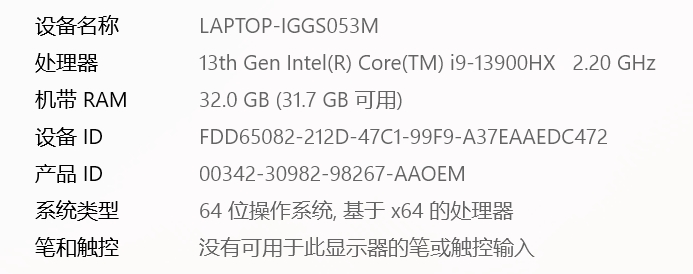
\includegraphics[width=0.8\textwidth]{./picture/设备.png}
\end{figure}

\subsection{测试软件}

主流浏览器（Chrome、Firefox、Safari、Edge等）。

\section{模块功能测试}

\subsection{用户账户模块}

\subsubsection{邮件发送}
输入合法的邮箱，可以正常接收到邮件。
\begin{figure}[H]
  \centering
  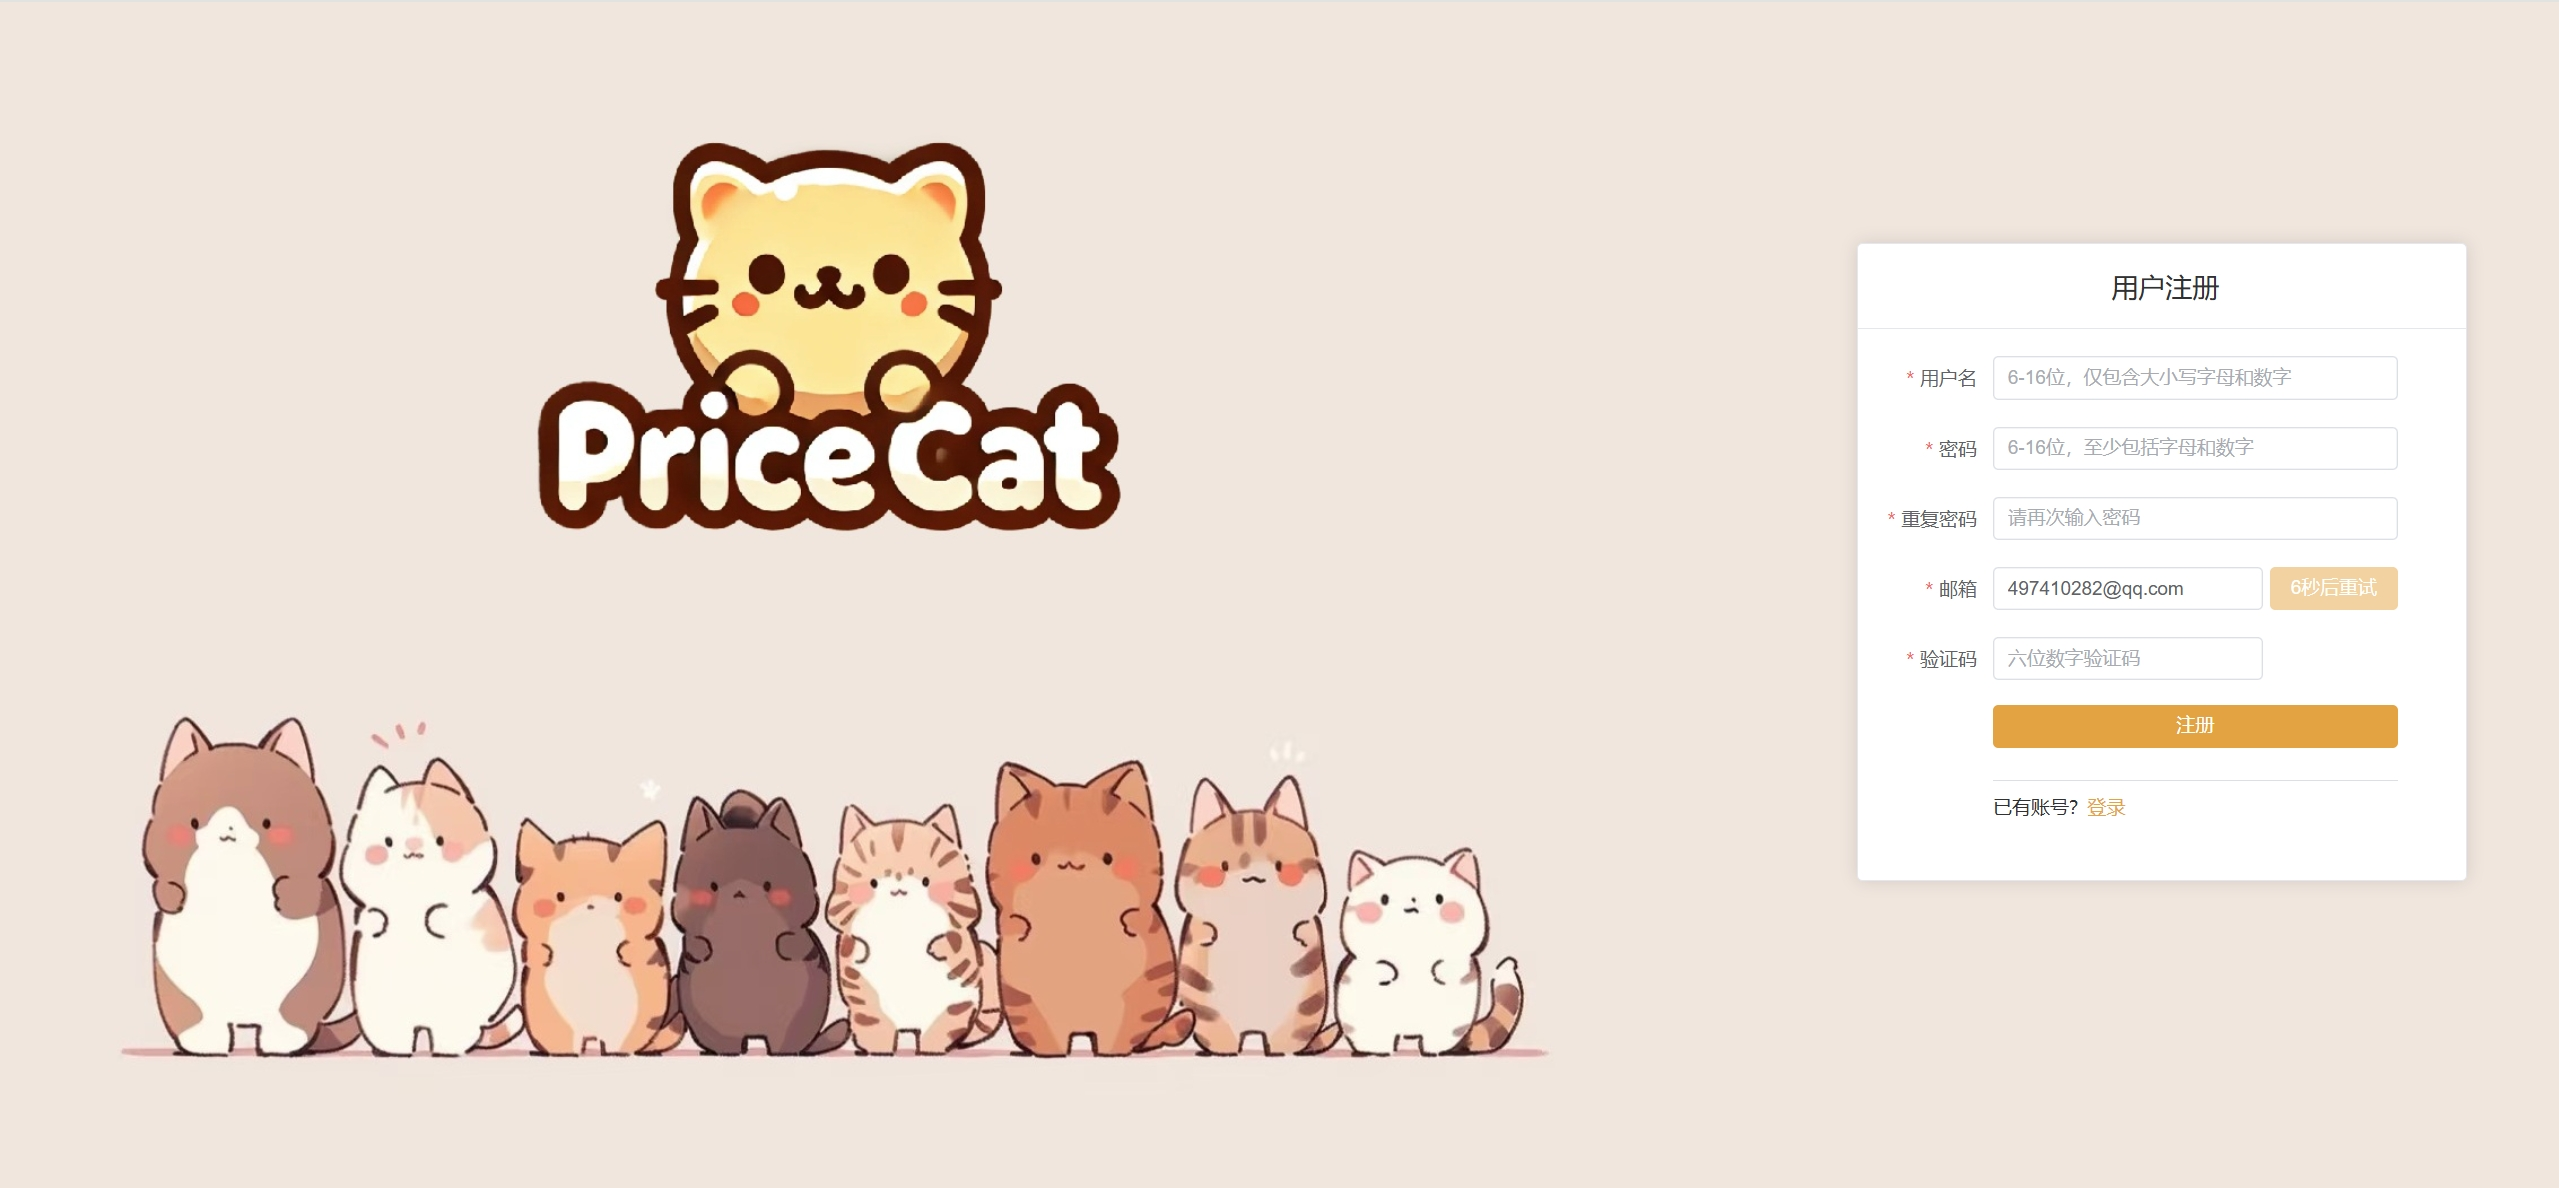
\includegraphics[width=1\textwidth]{./picture/邮件发送.png}
\end{figure}

\begin{figure}[H]
  \centering
  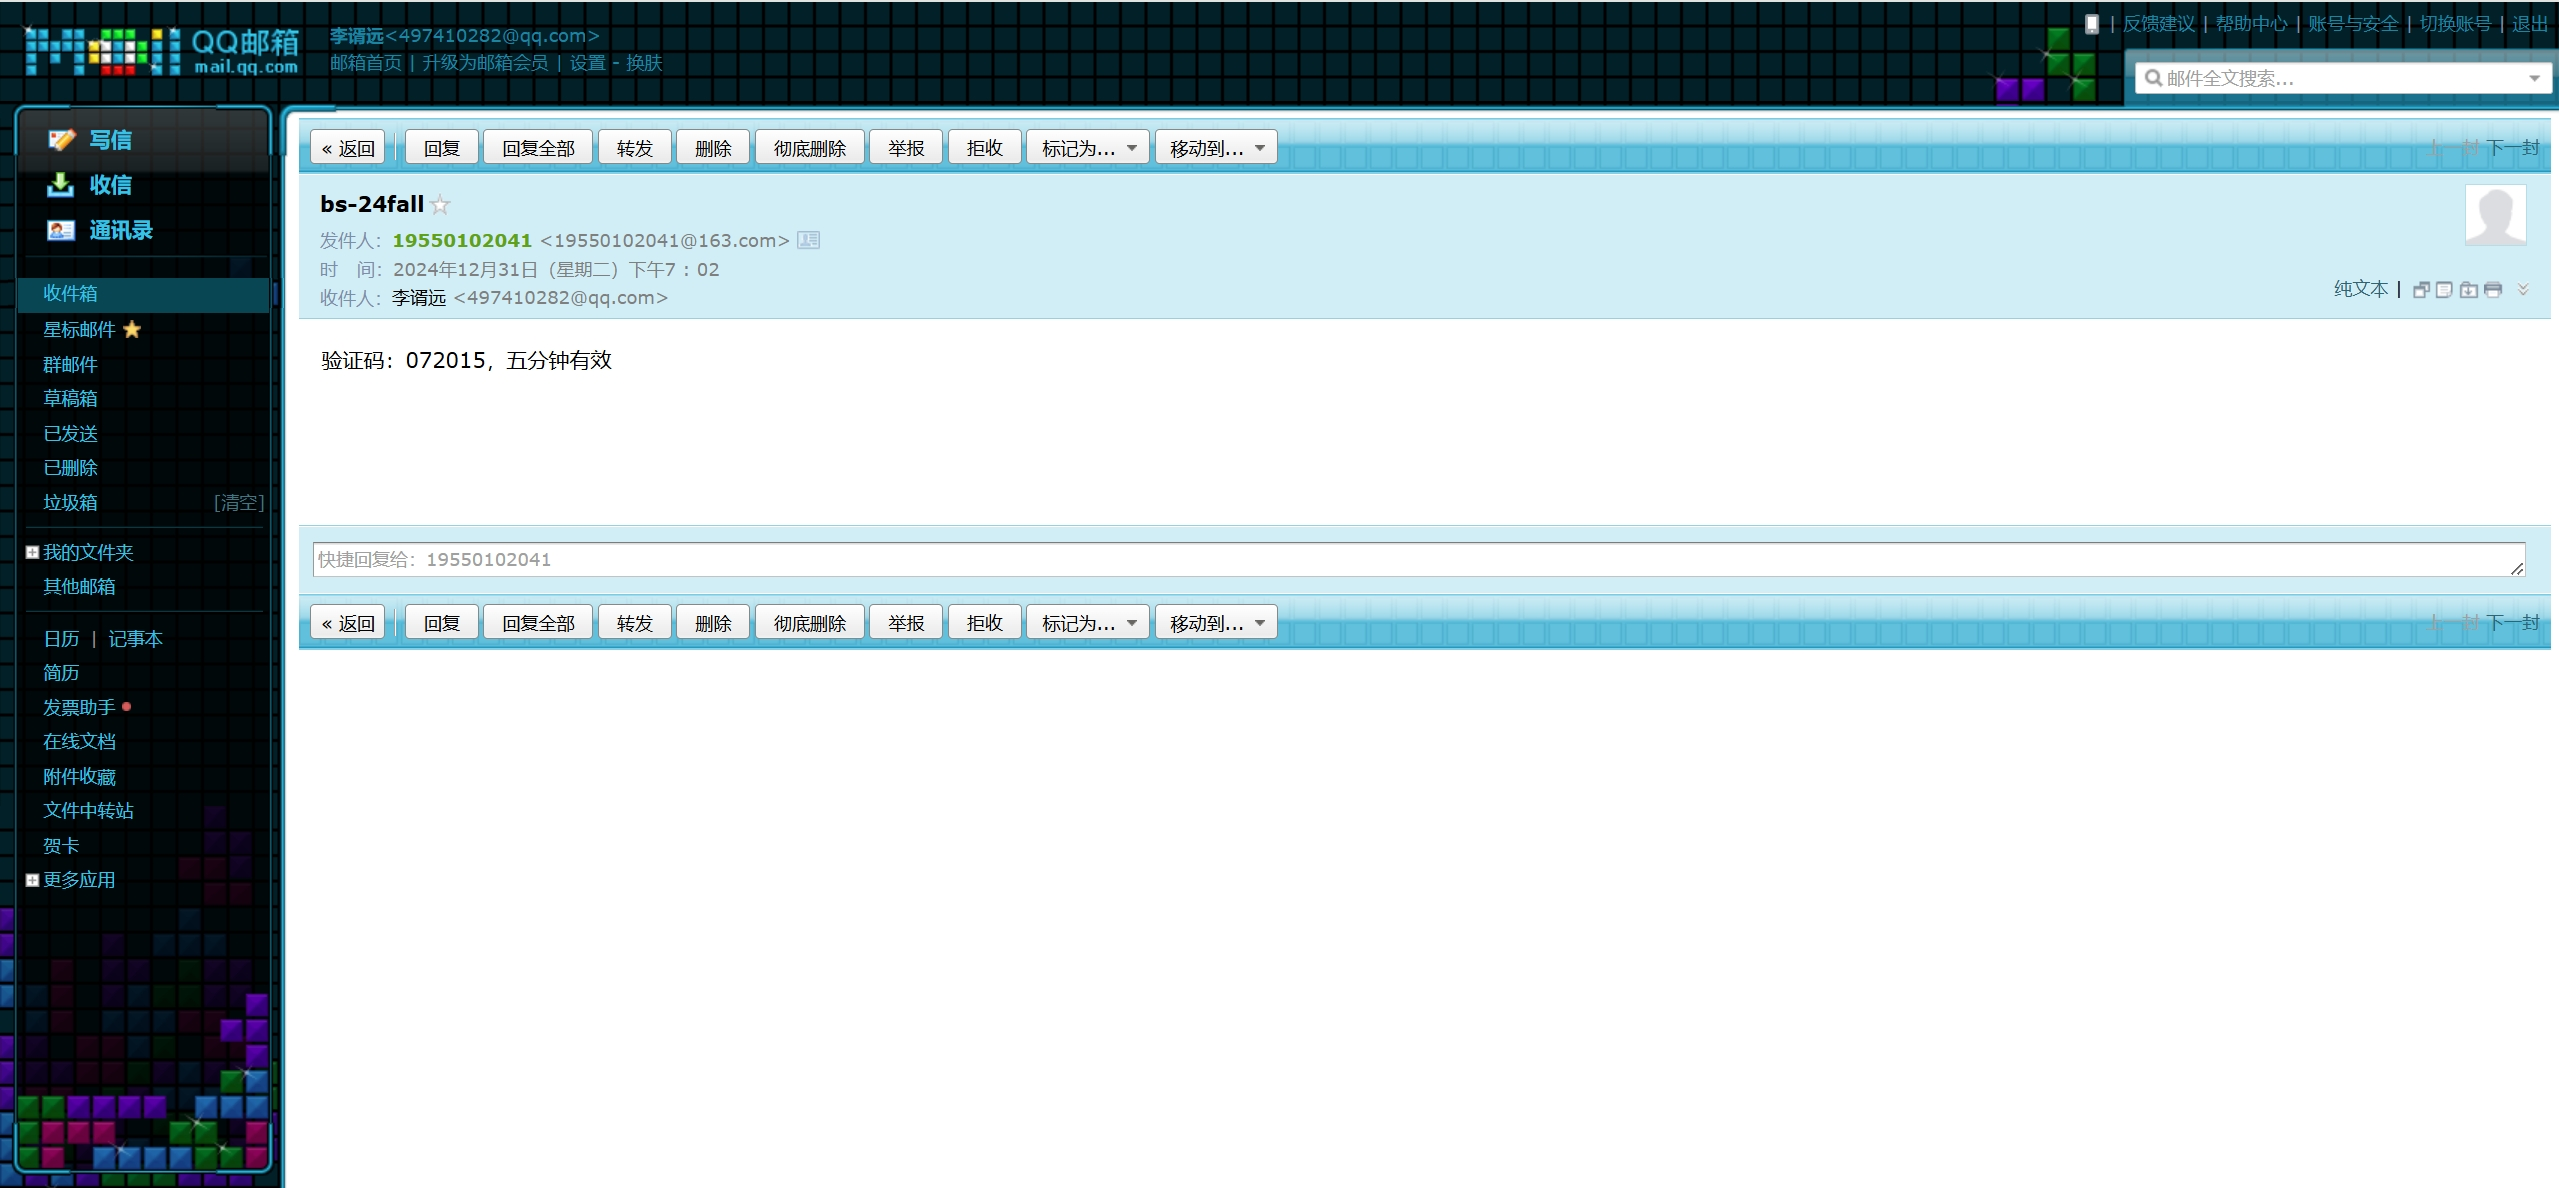
\includegraphics[width=1\textwidth]{./picture/邮件接收.png}
\end{figure}

\subsubsection{用户注册}
输入合法的用户名、密码、邮箱地址和验证码，可以成功注册。
\begin{figure}[H]
  \centering
  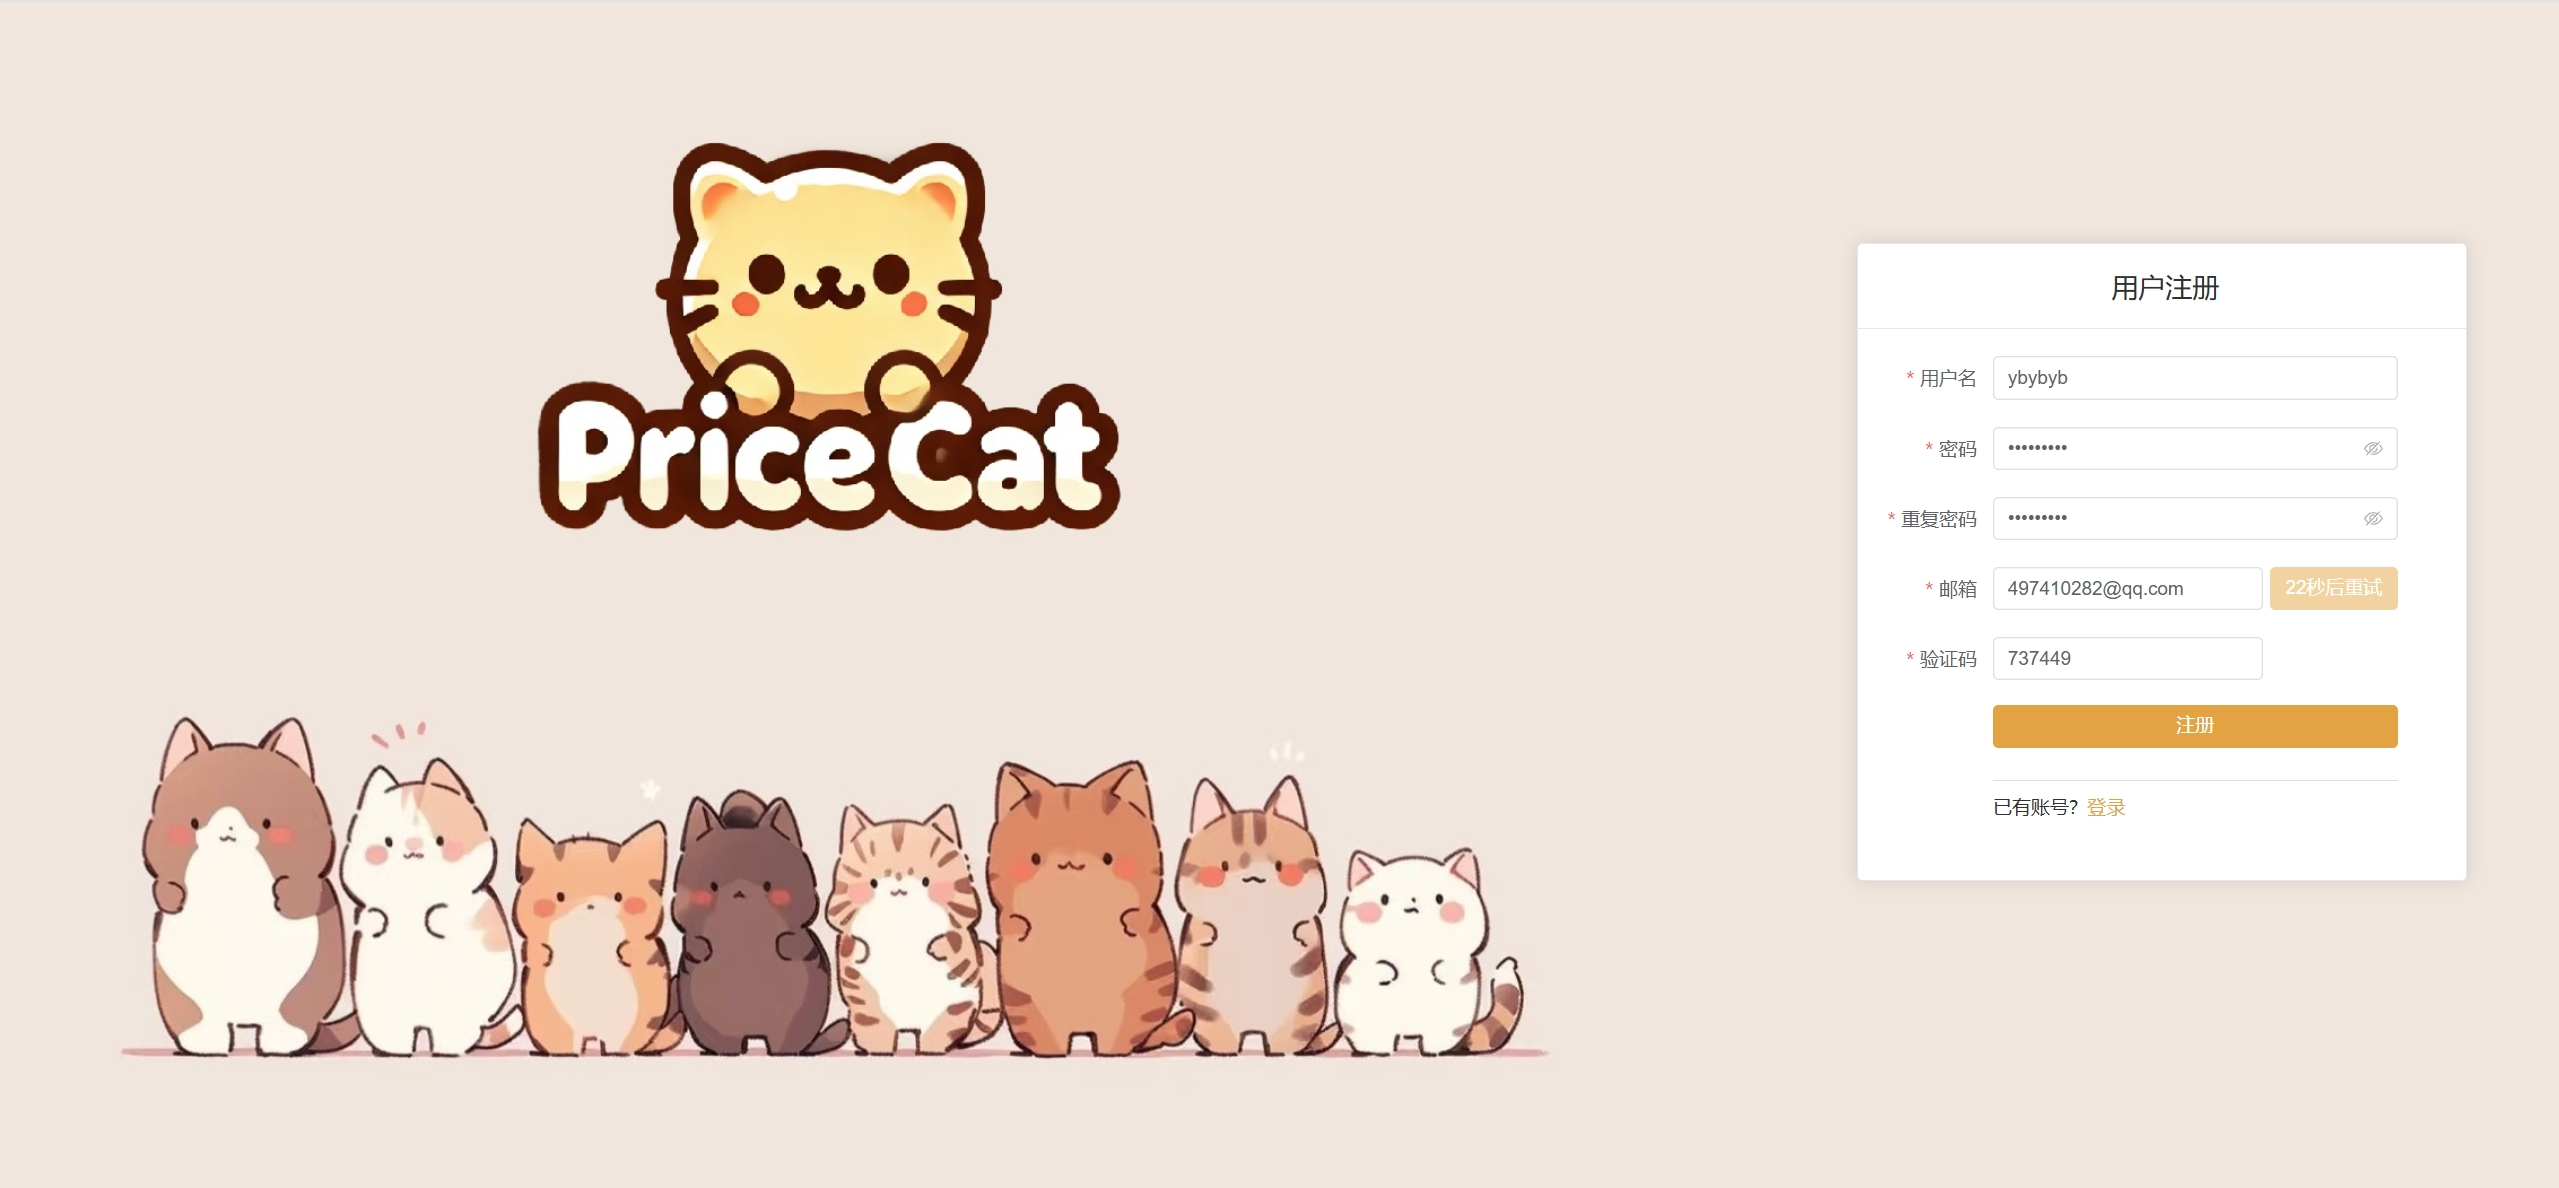
\includegraphics[width=1\textwidth]{./picture/用户注册.png}
\end{figure}

\subsubsection{用户登录}
输入正确的用户名和密码，可以成功登录。
\begin{figure}[H]
  \centering
  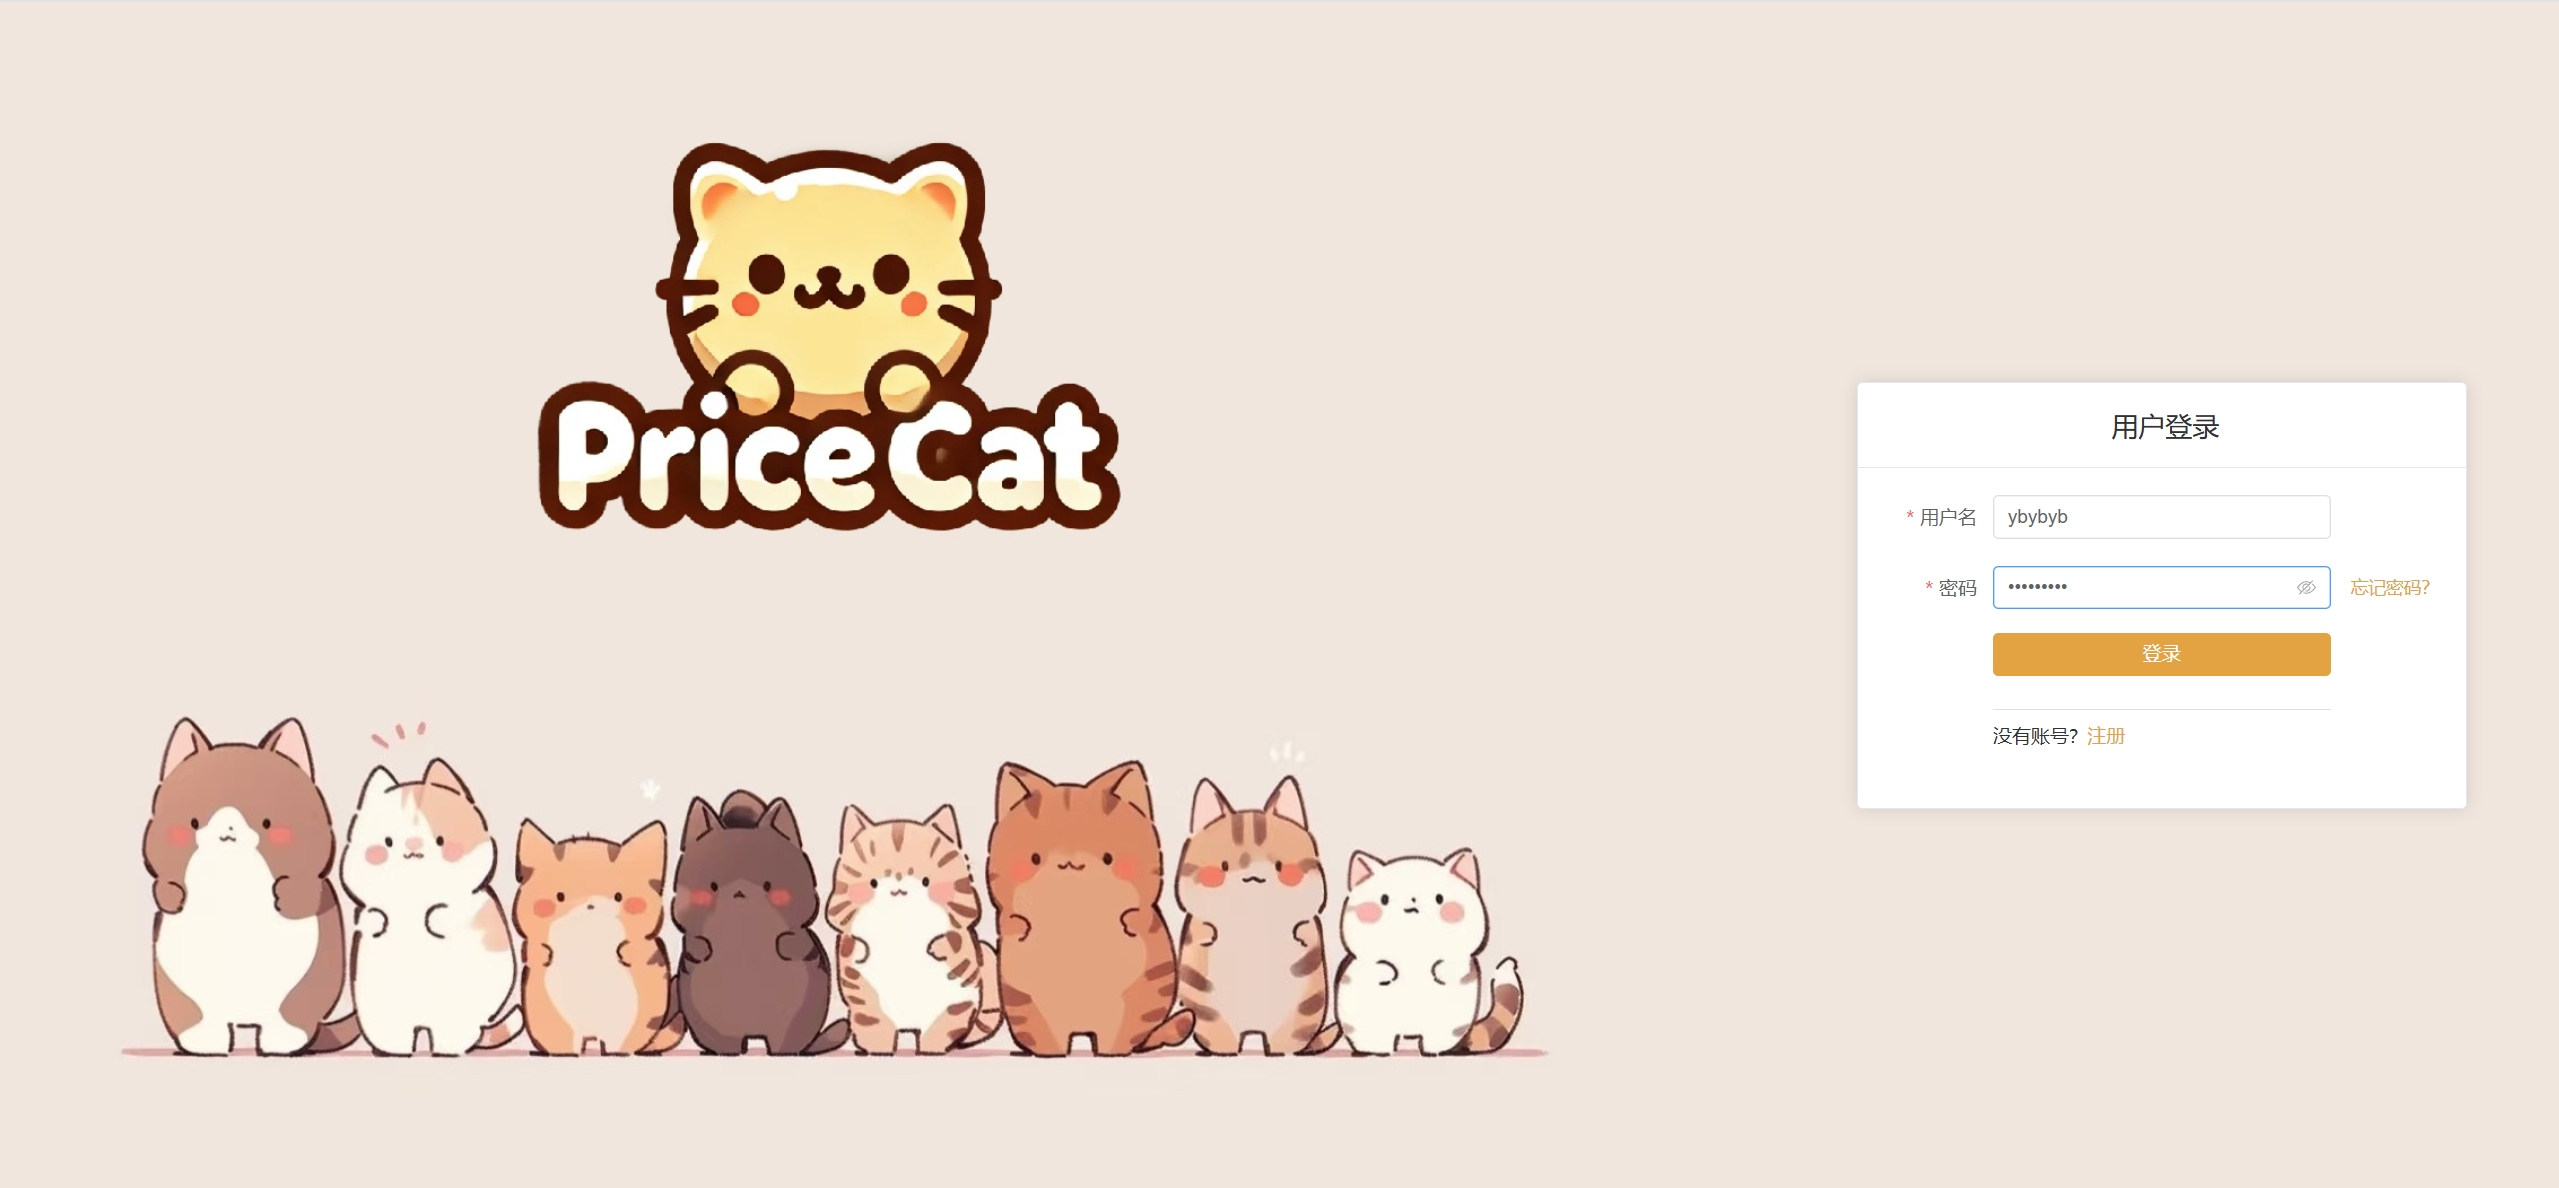
\includegraphics[width=1\textwidth]{./picture/用户登录.png}
\end{figure}

\subsubsection{忘记密码}
输入合法的邮箱地址和验证码，可以成功修改密码。
\begin{figure}[H]
  \centering
  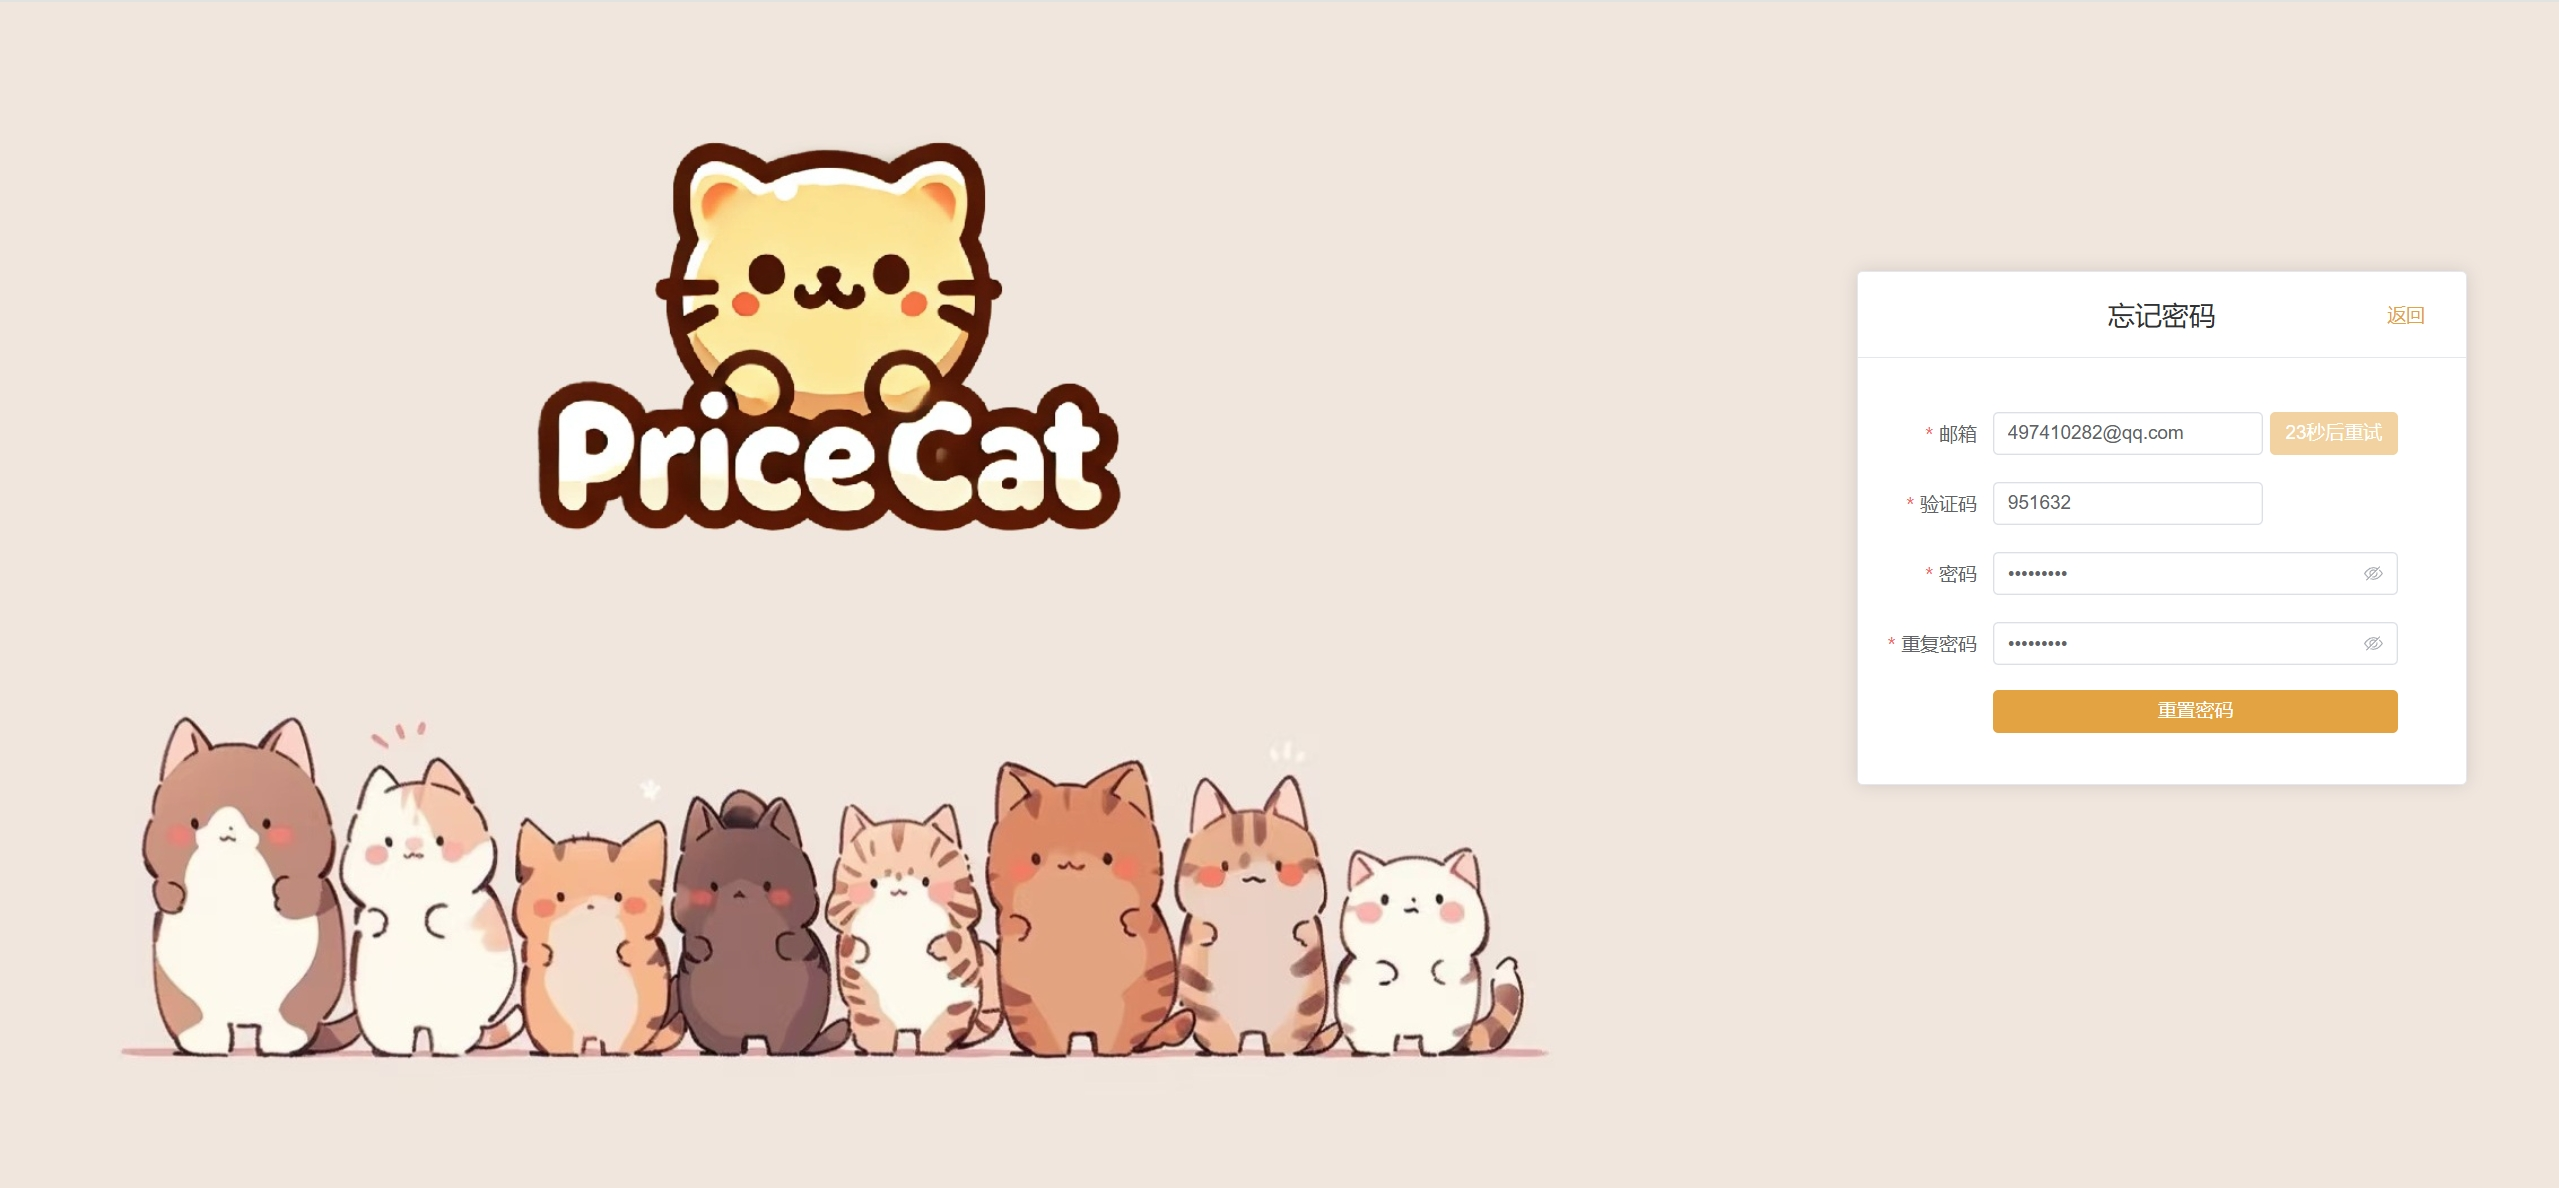
\includegraphics[width=1\textwidth]{./picture/忘记密码.png}
\end{figure}

\subsubsection{用户主页}
登录后可以查看用户主页，能正确展示用户信息。
\begin{figure}[H]
  \centering
  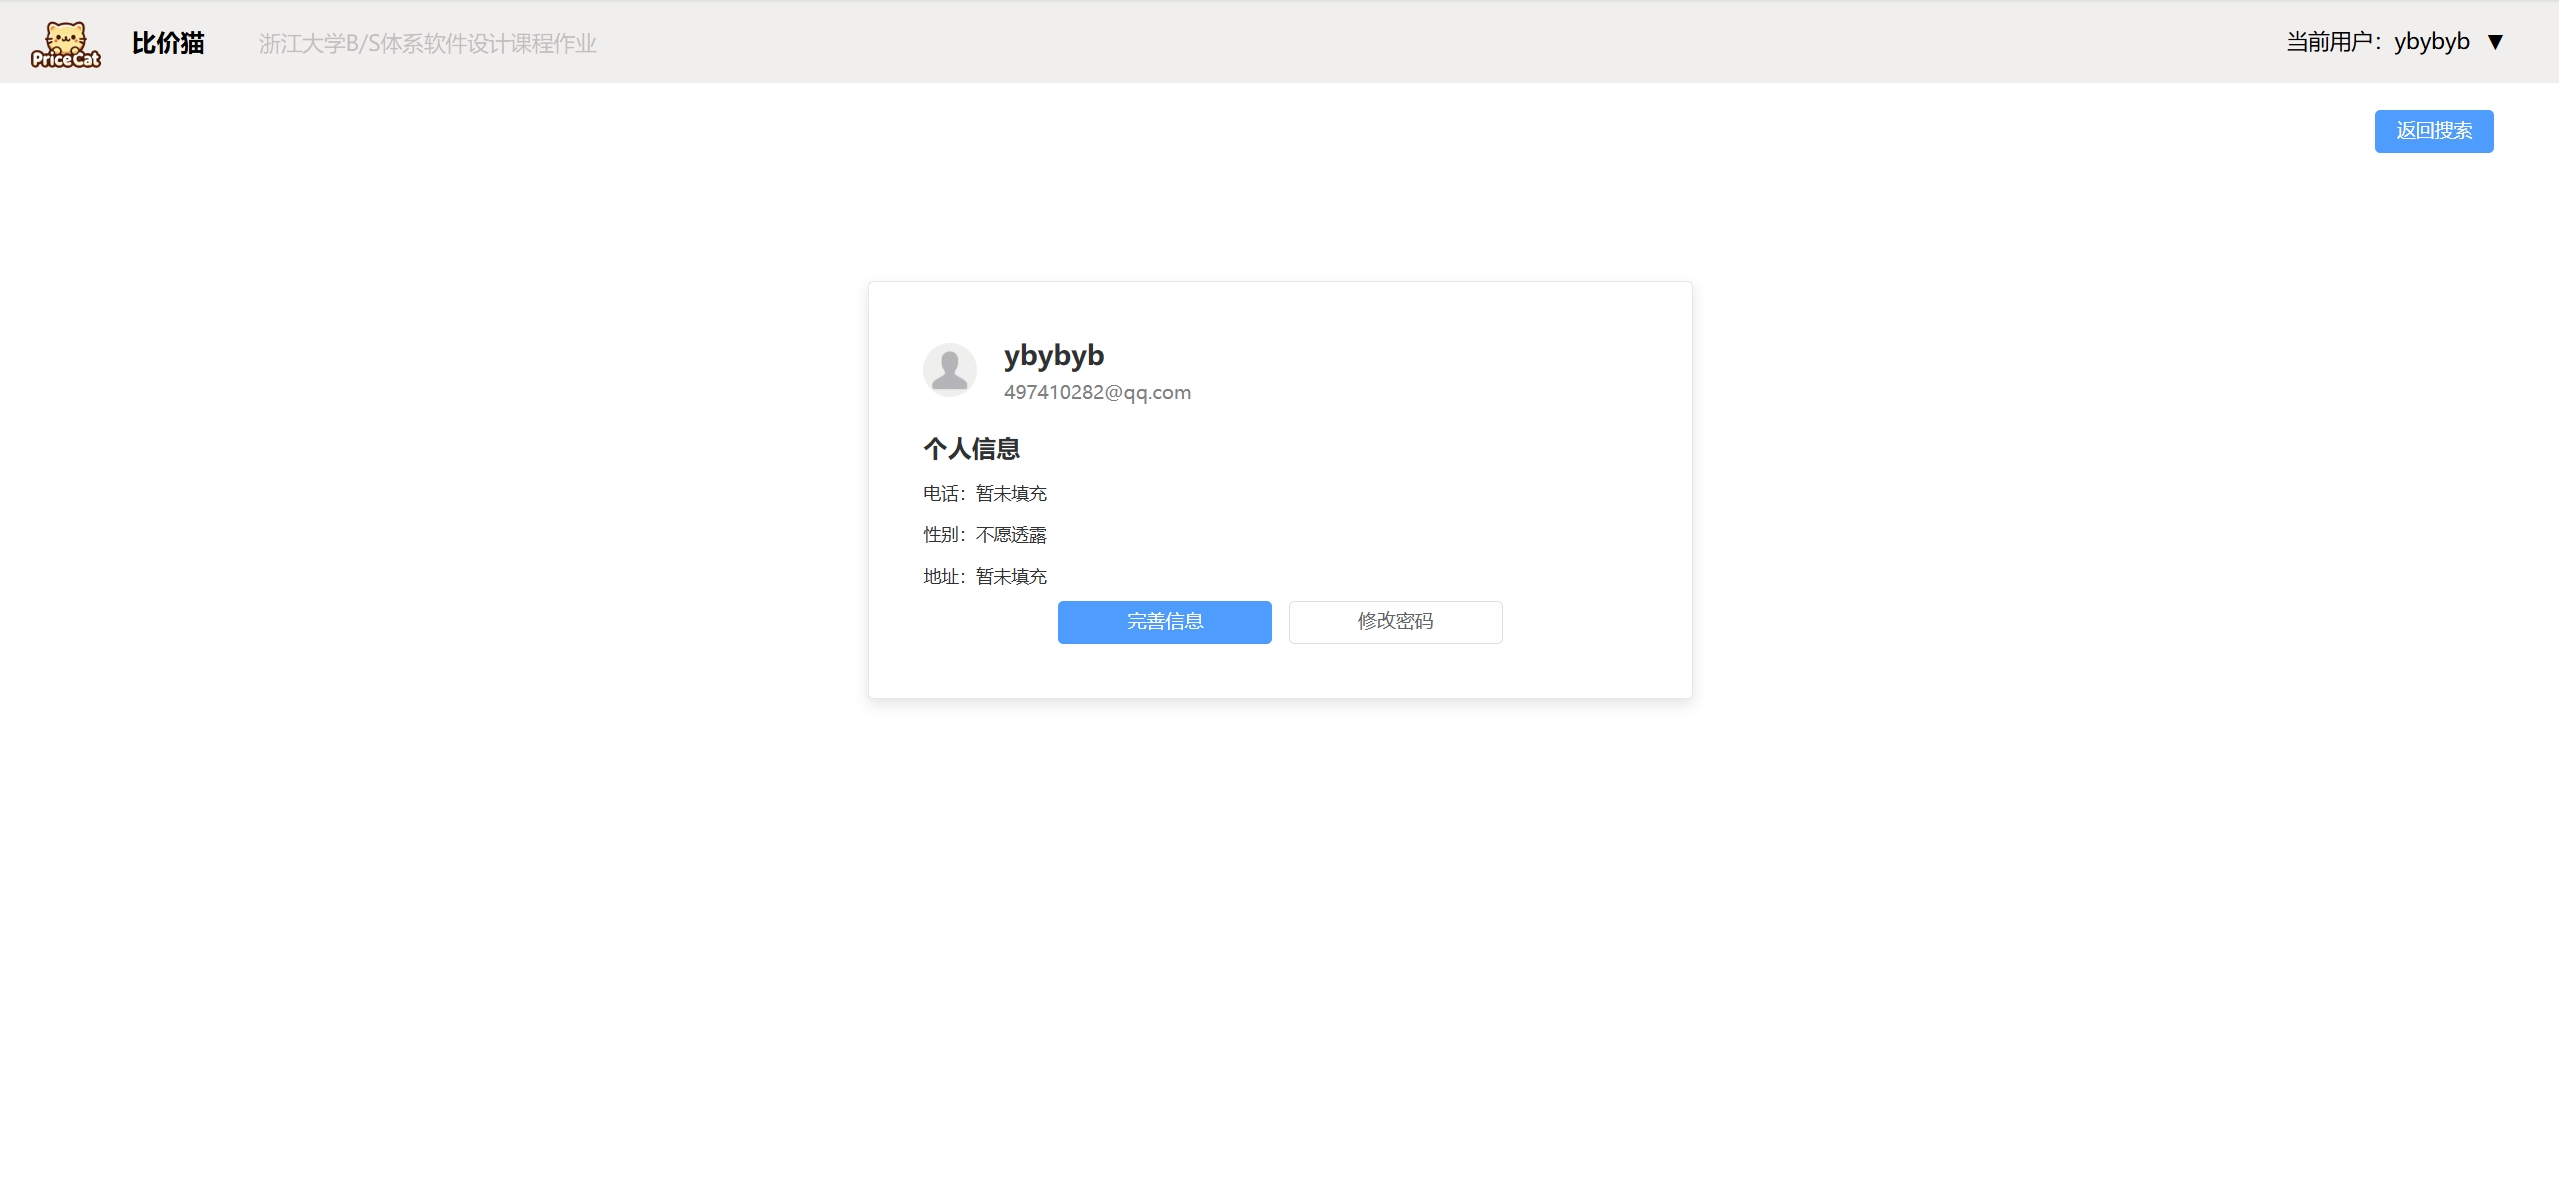
\includegraphics[width=1\textwidth]{./picture/用户主页.png}
\end{figure}

\subsubsection{用户信息修改}
可以修改用户信息，修改后能正确展示。
\begin{figure}[H]
  \centering
  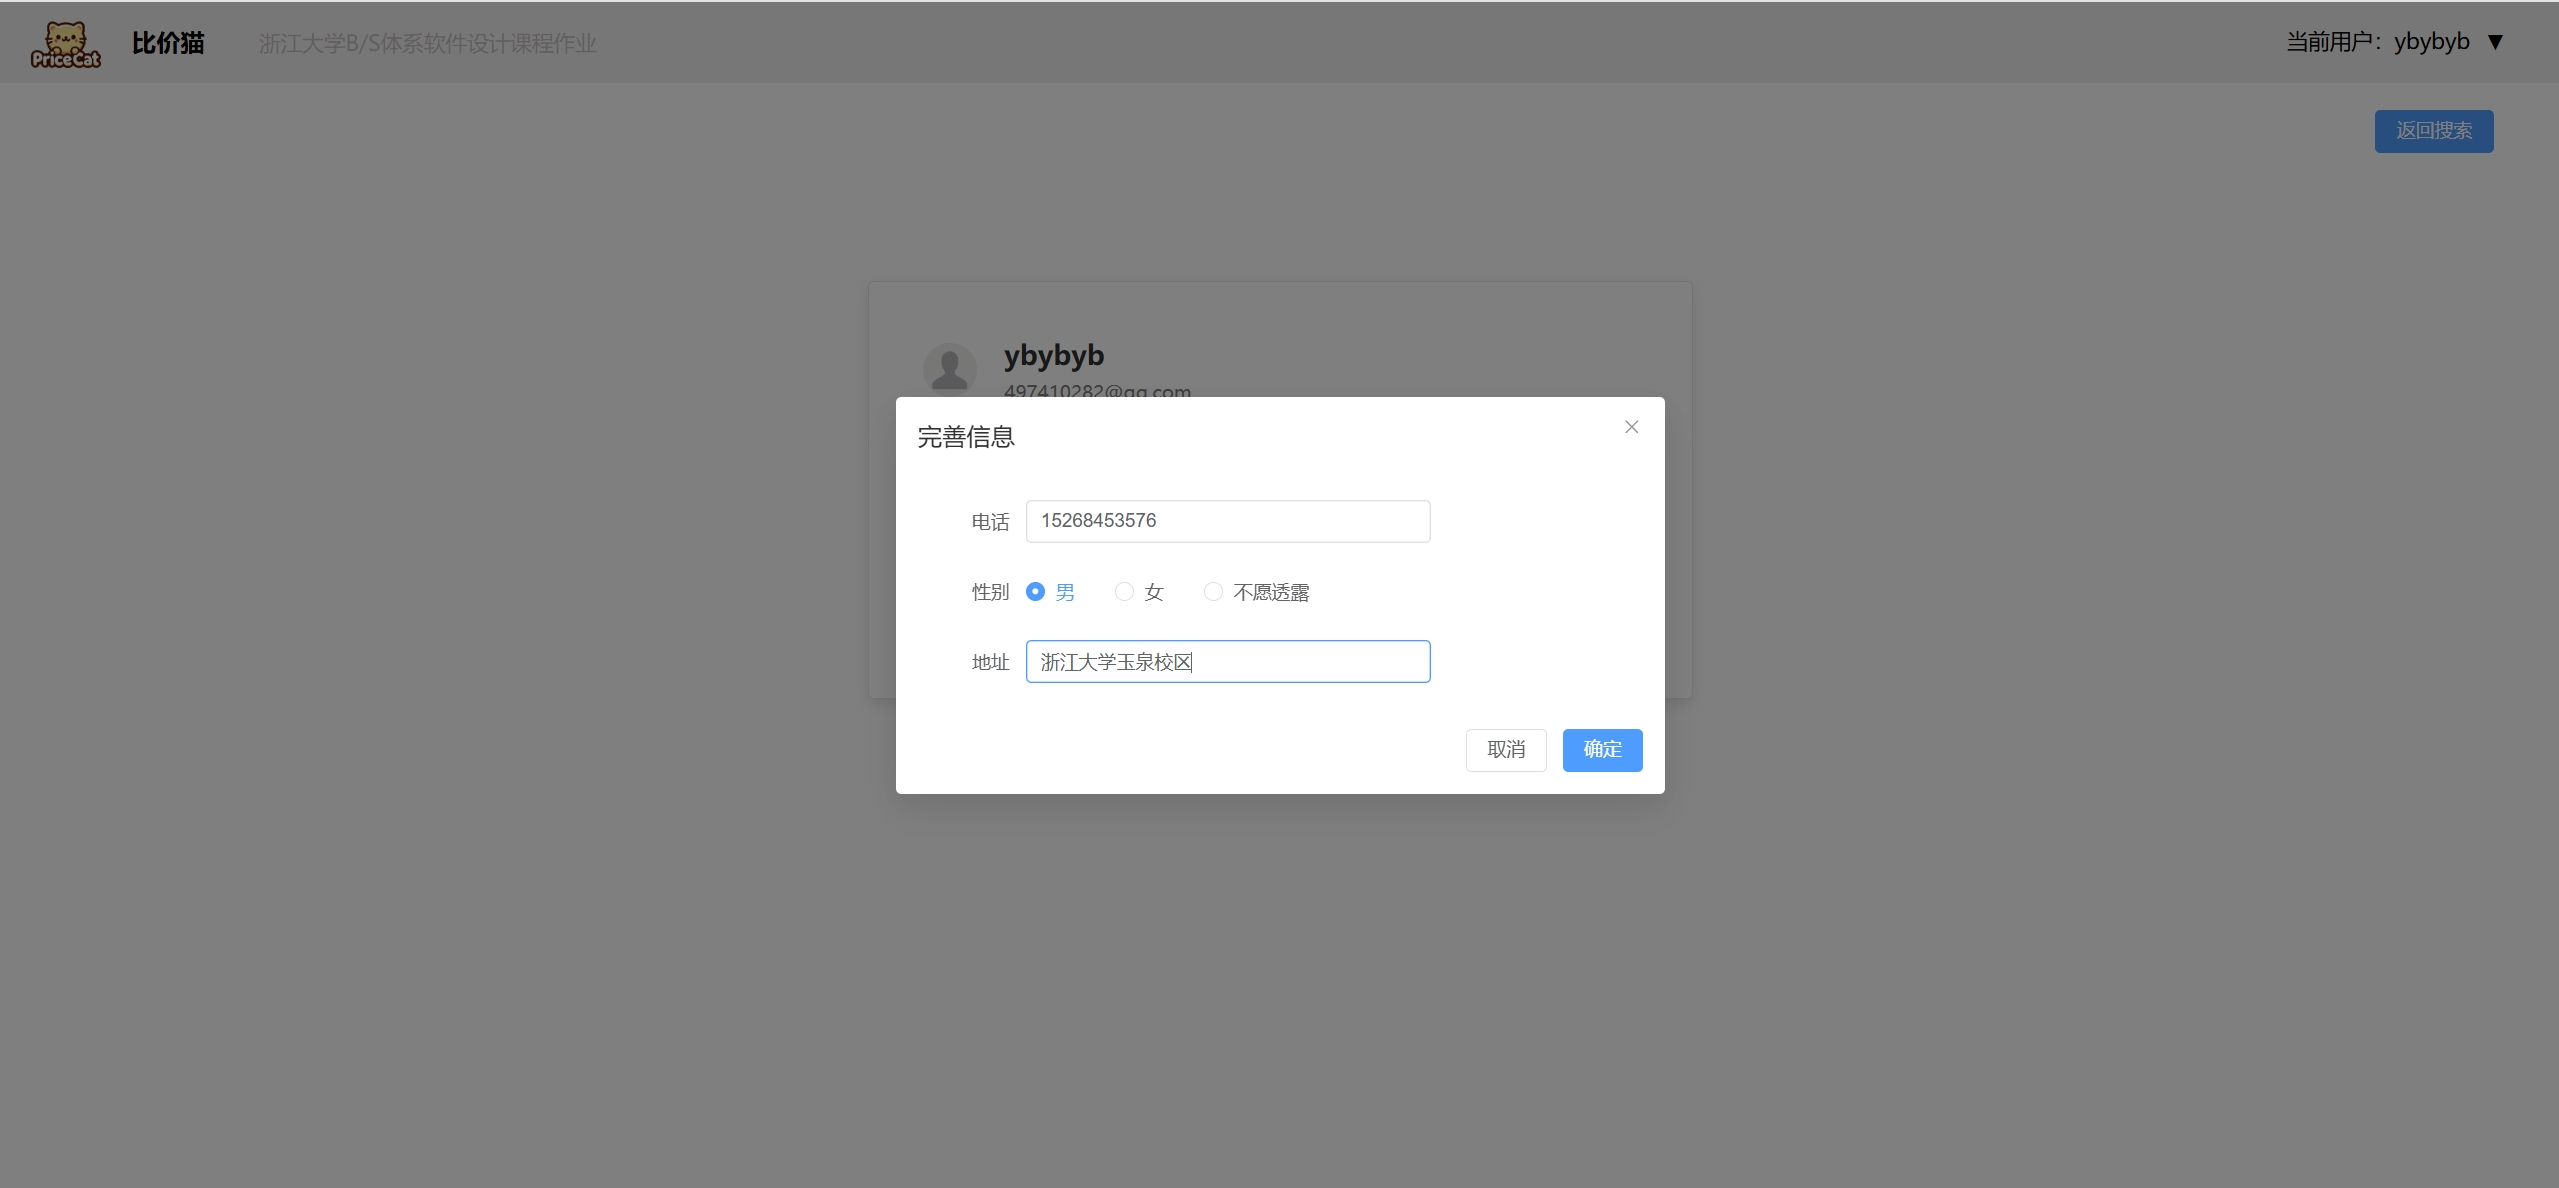
\includegraphics[width=1\textwidth]{./picture/用户信息修改.png}
\end{figure}

\subsection{商品模块}

\subsubsection{商品查询}
输入商品名称，选择京东平台，可以查询到商品信息。
\begin{figure}[H]
  \centering
  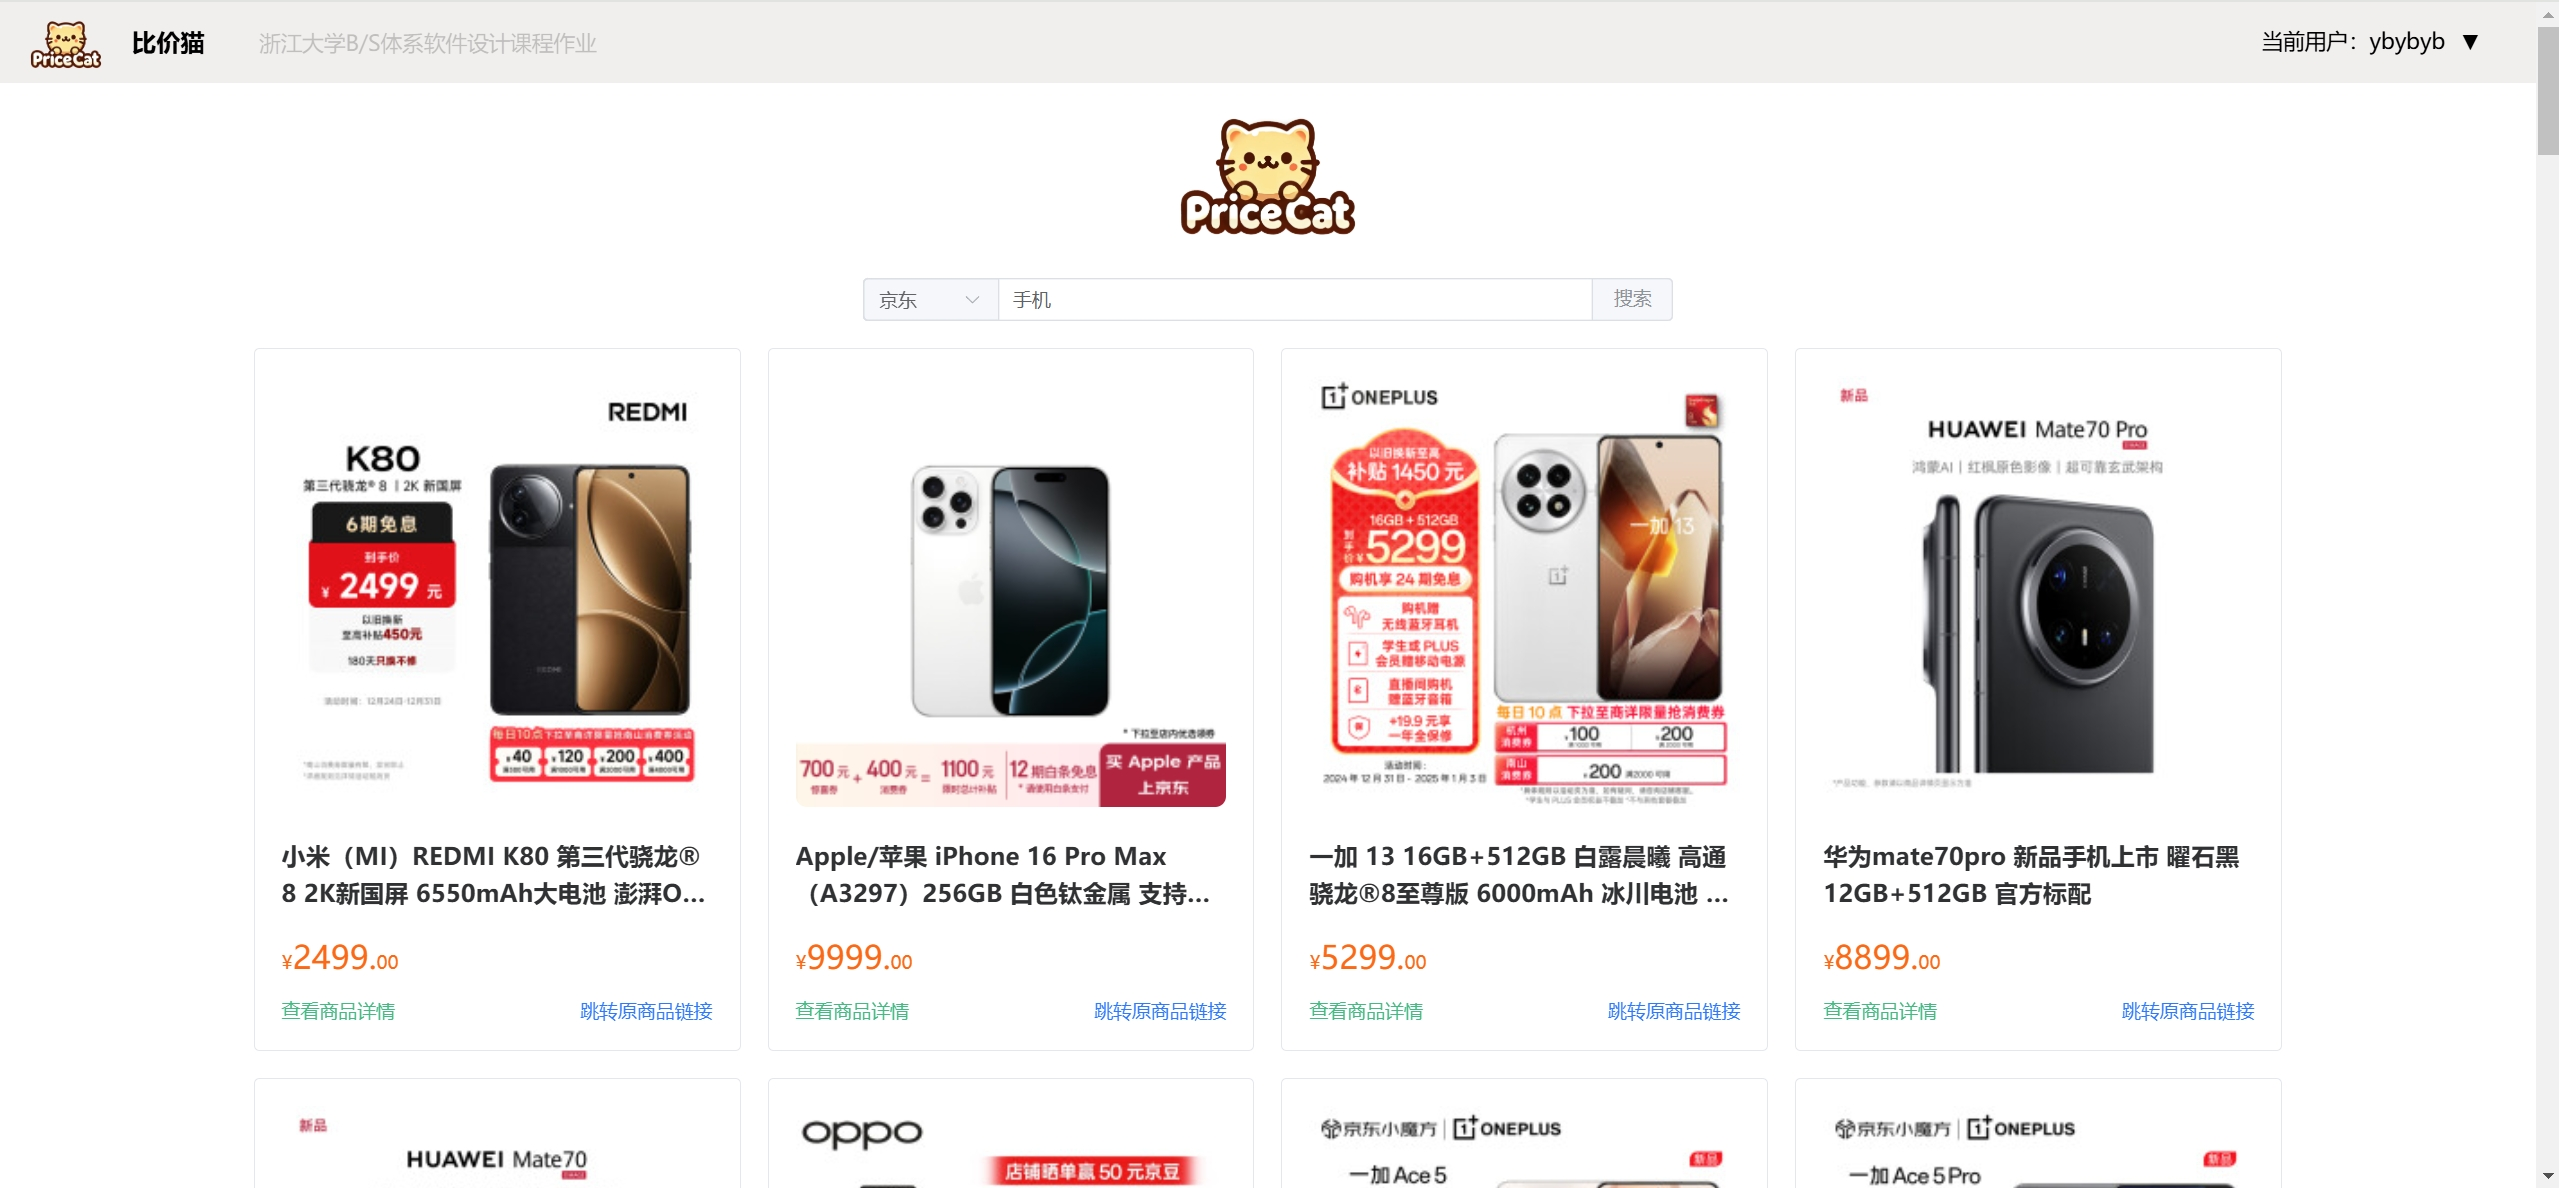
\includegraphics[width=1\textwidth]{./picture/商品查询1.png}
\end{figure}

输入商品名称，选择苏宁易购平台，可以查询到商品信息。
\begin{figure}[H]
  \centering
  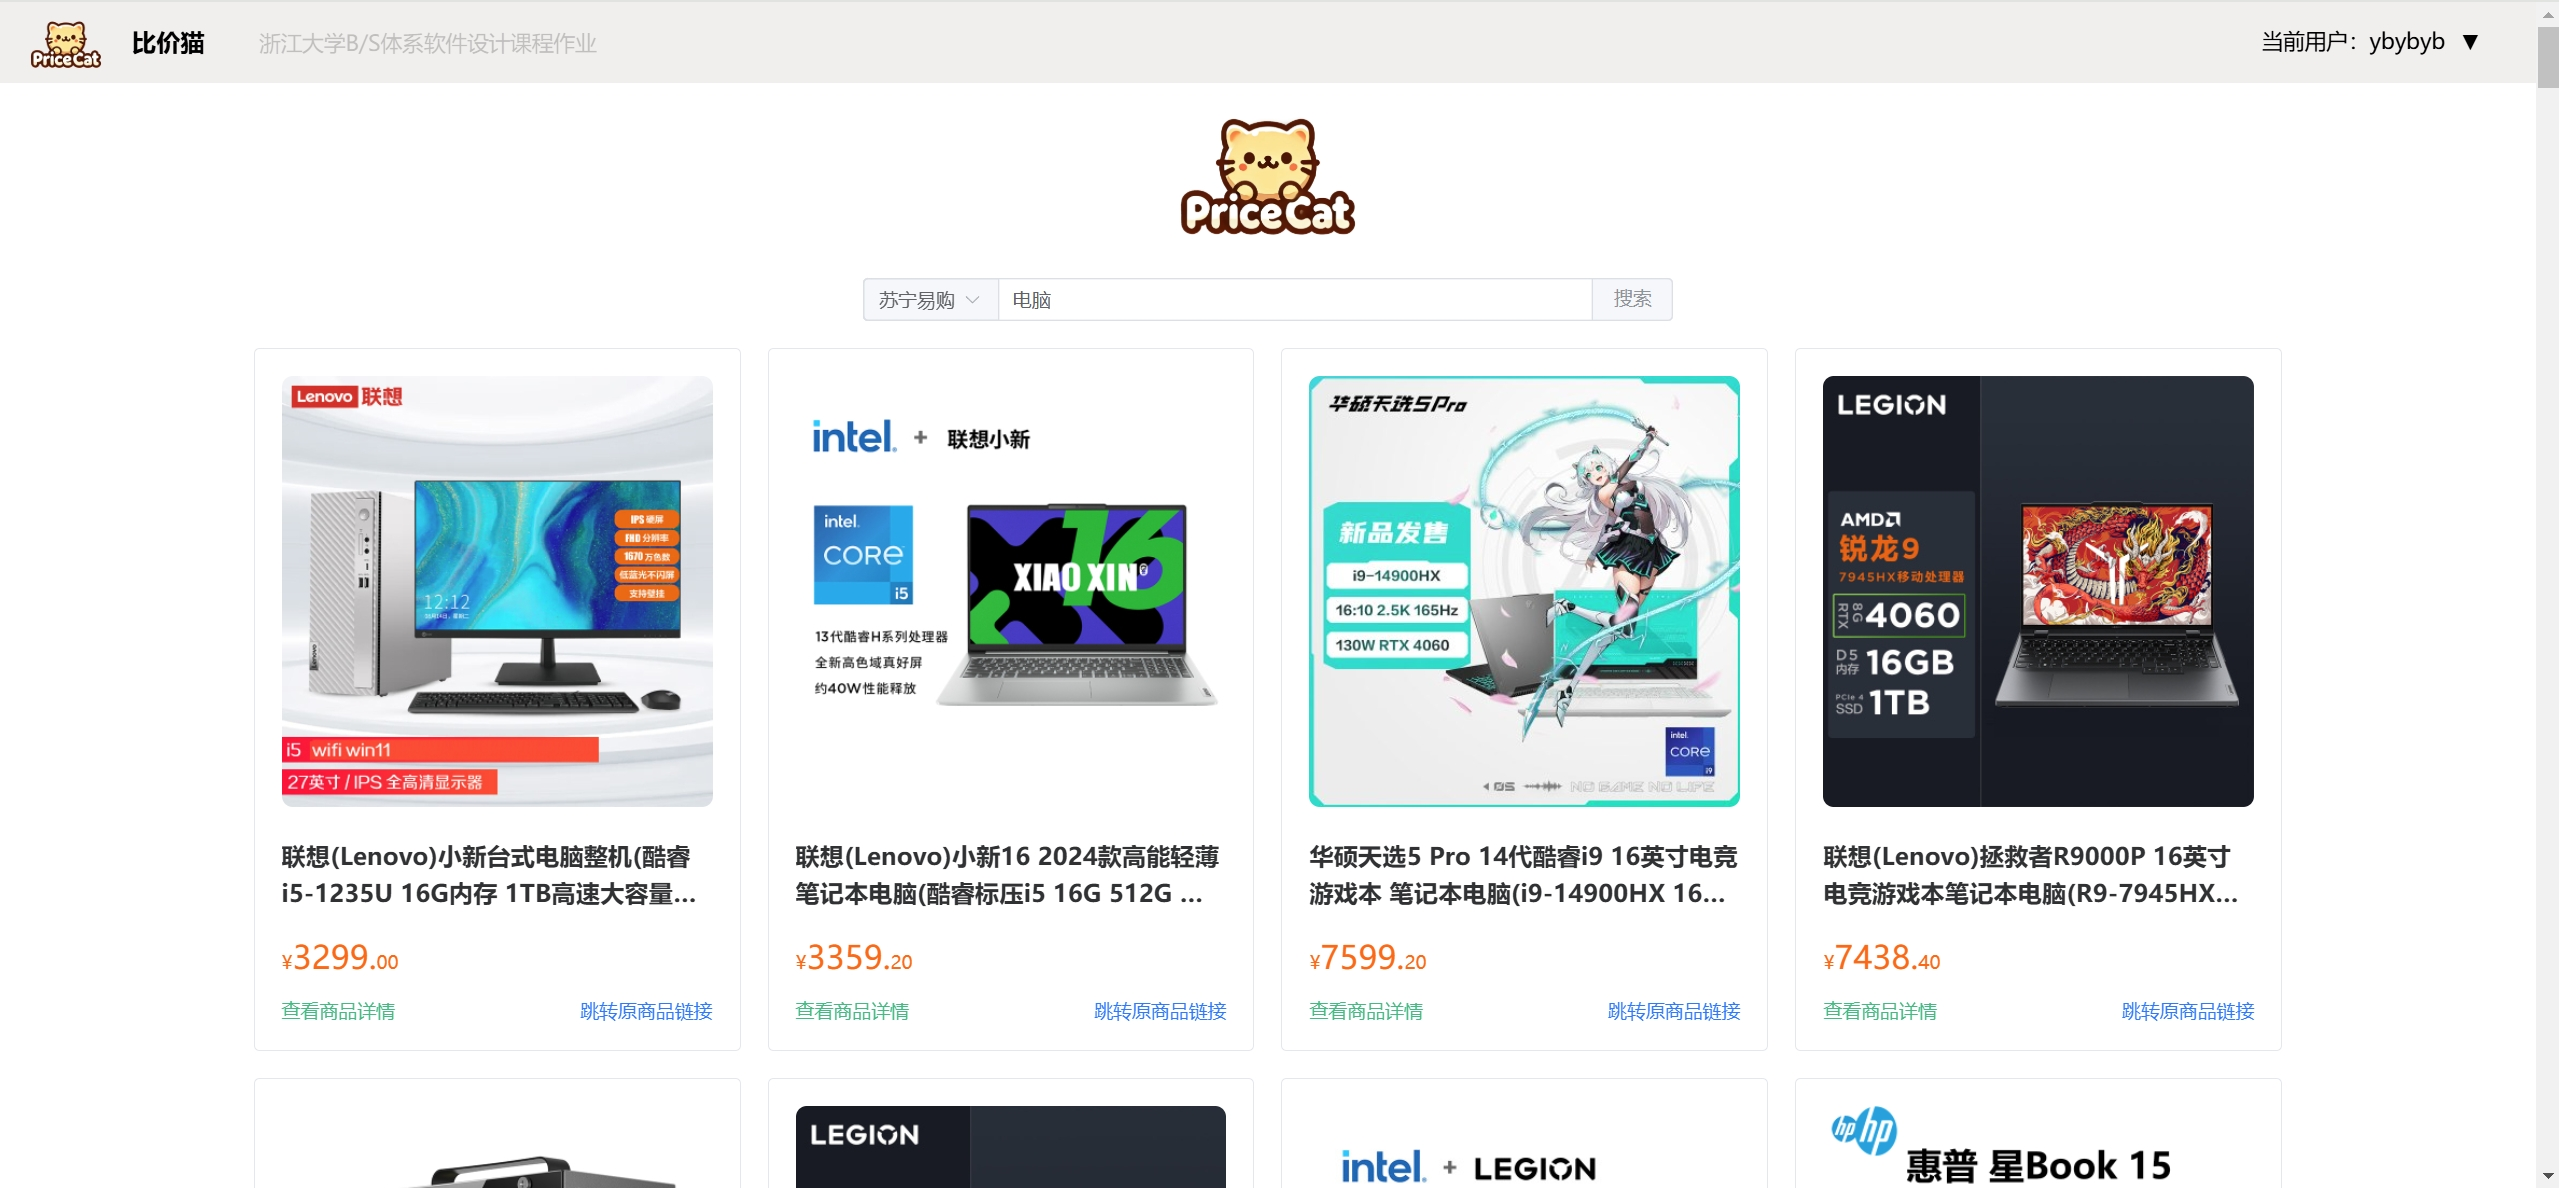
\includegraphics[width=1\textwidth]{./picture/商品查询2.png}
\end{figure}

\subsubsection{商品详情}
点击商品名称，可以查看商品详情和历史价格。
\begin{figure}[H]
  \centering
  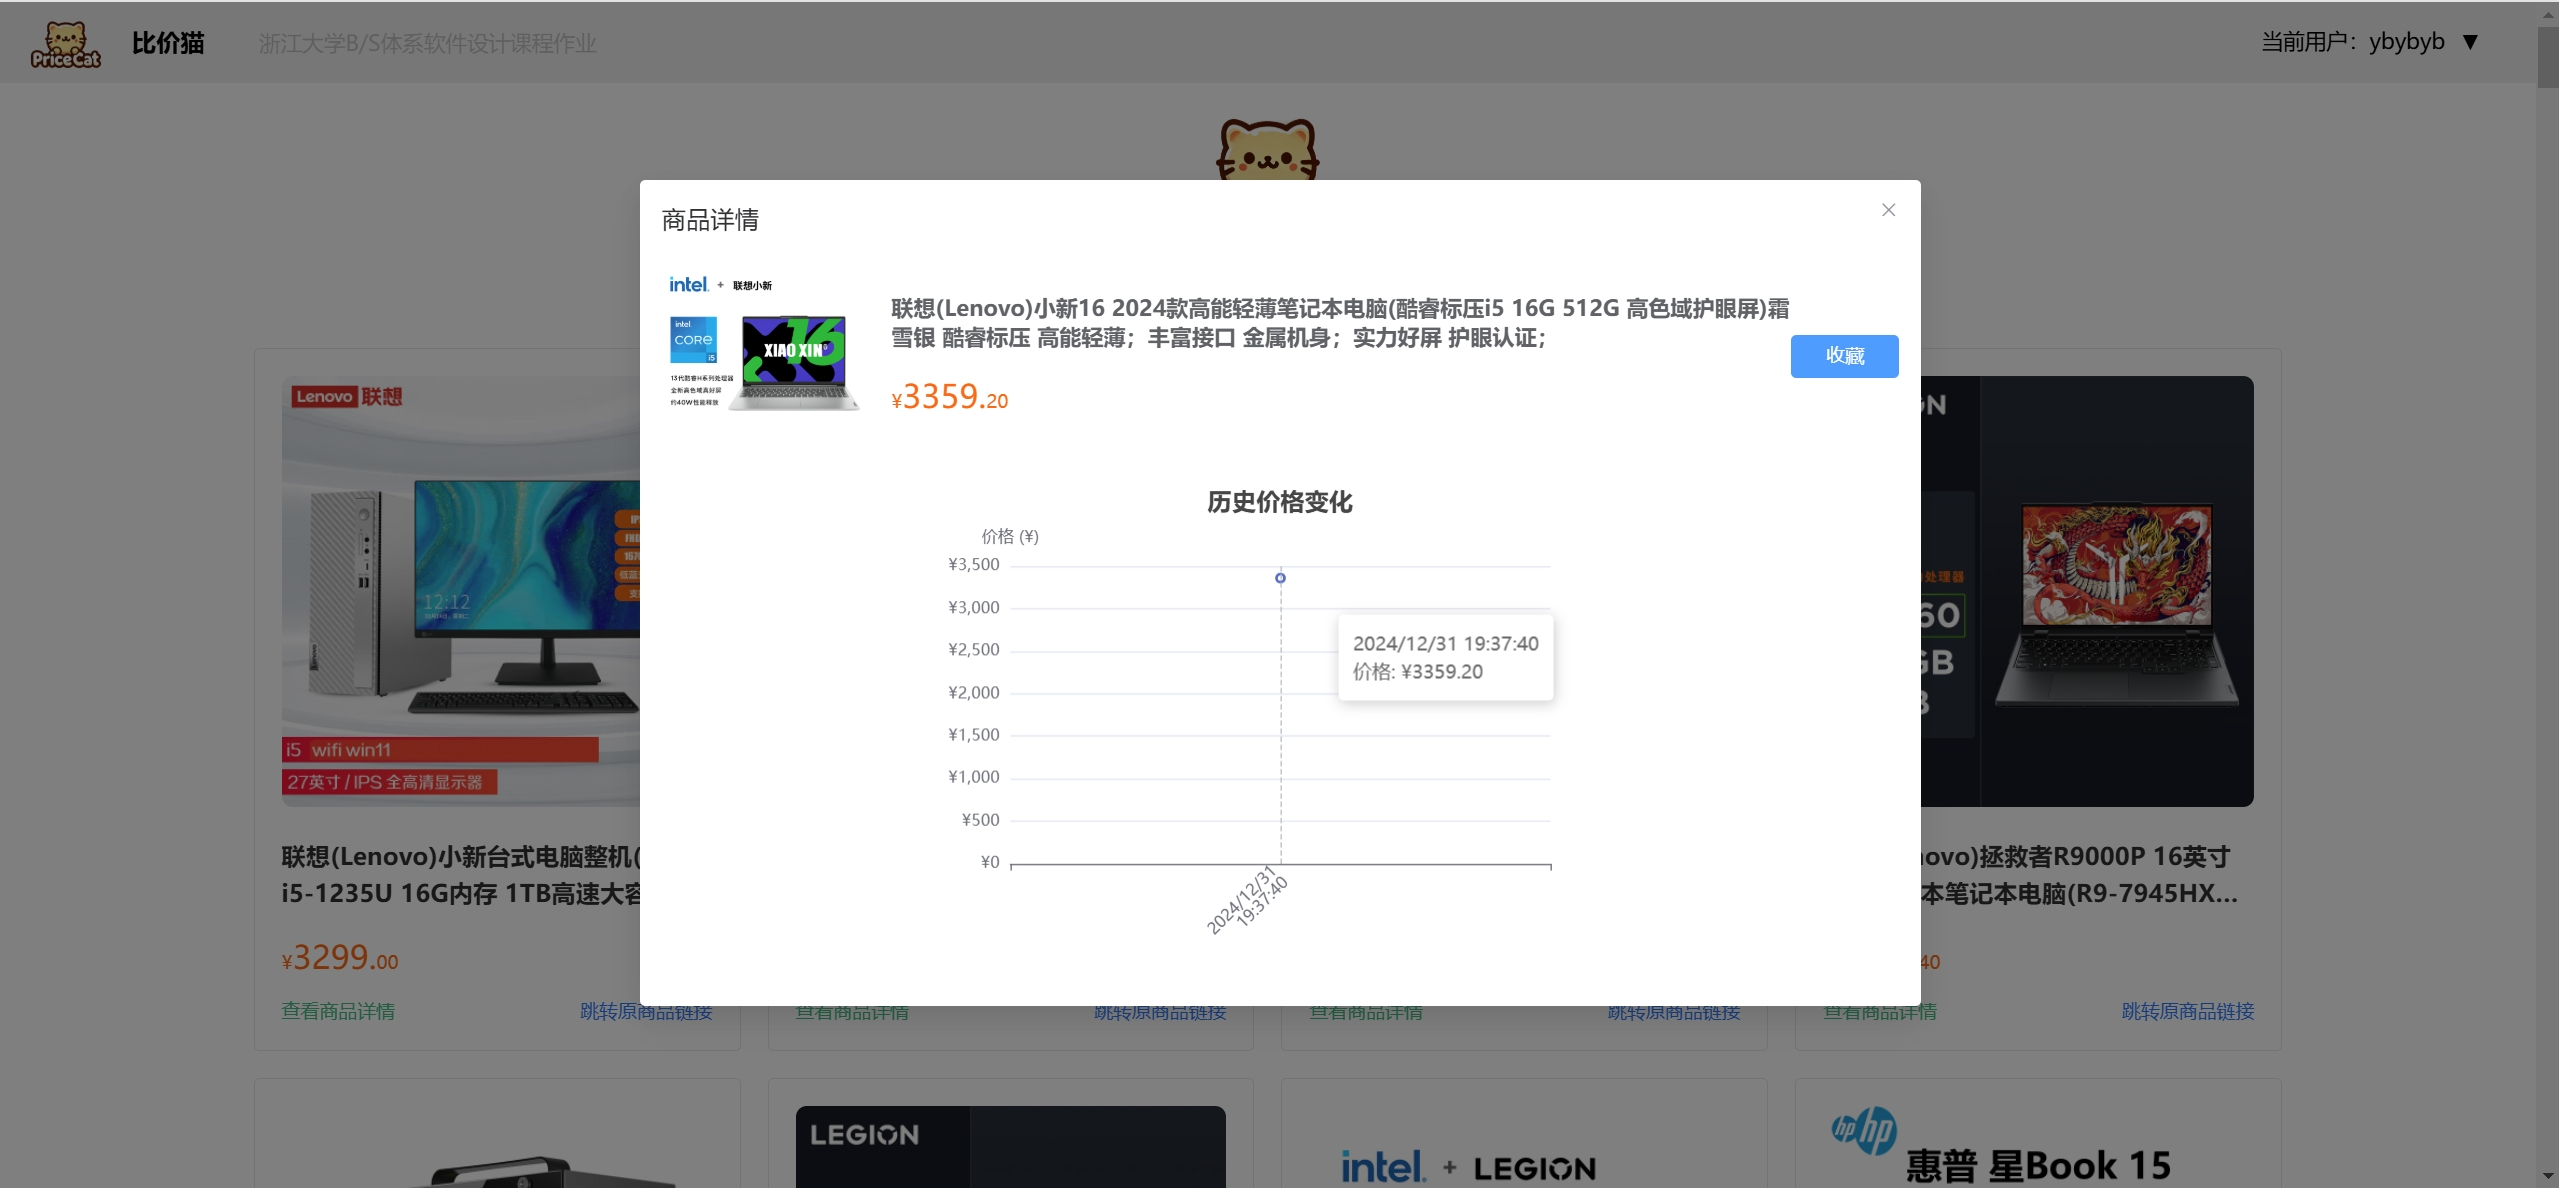
\includegraphics[width=1\textwidth]{./picture/商品详情1.png}
\end{figure}

点击跳转原商品链接，可以跳转到对应商品的原链接。
\begin{figure}[H]
  \centering
  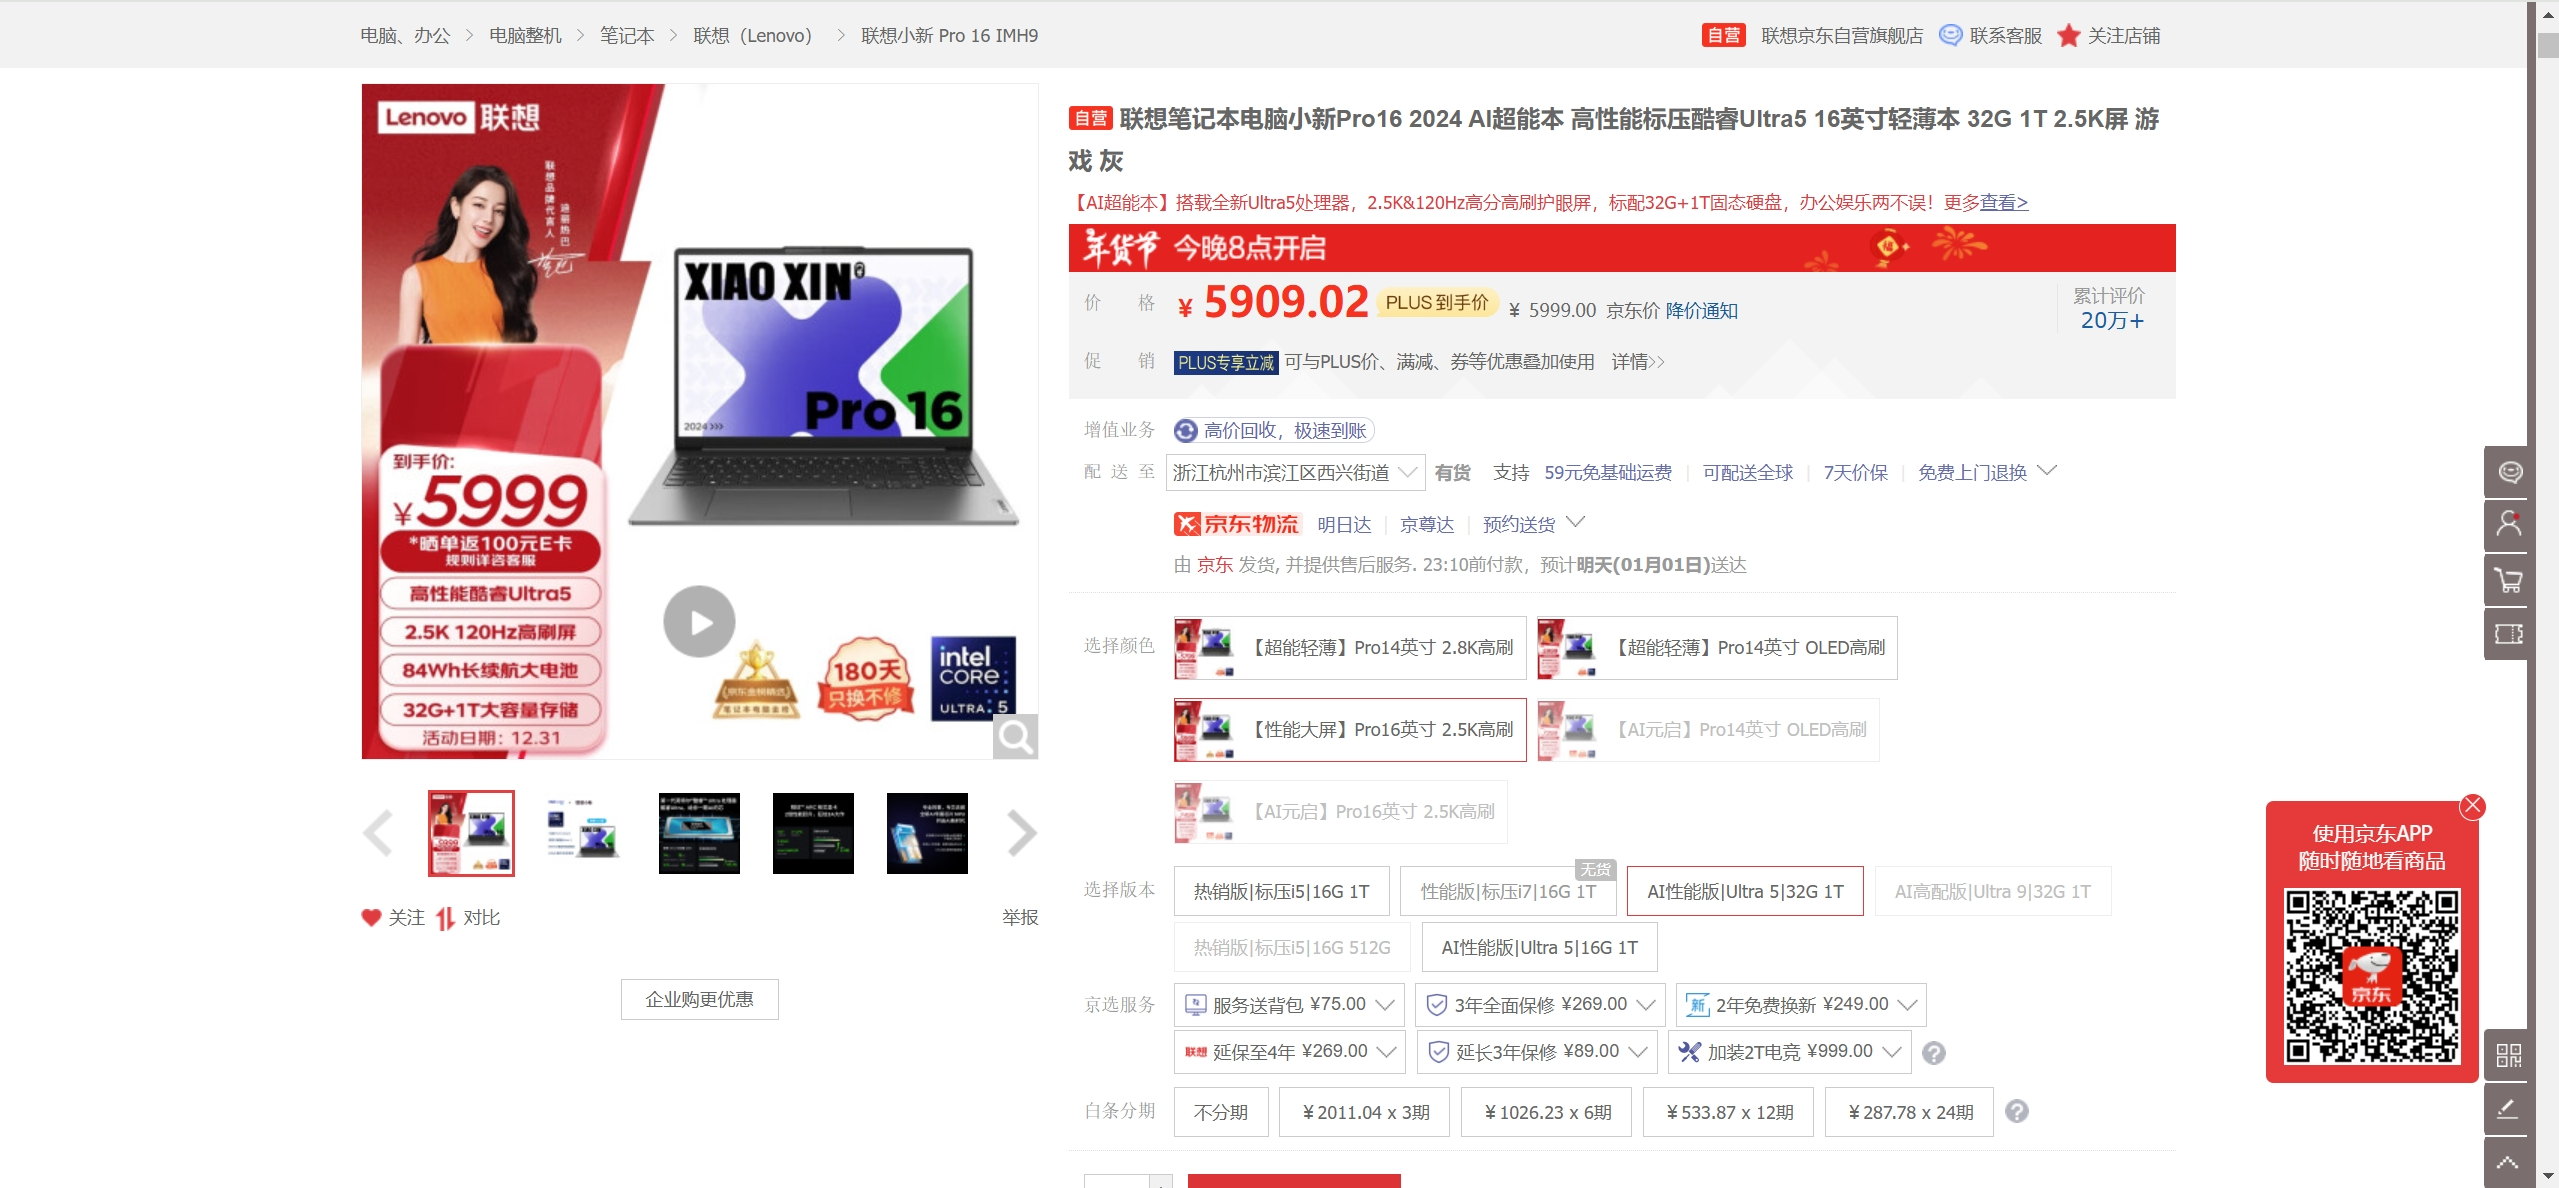
\includegraphics[width=1\textwidth]{./picture/商品详情2.png}
\end{figure}

\subsubsection{商品收藏}
点击收藏按钮，可以收藏商品。
\begin{figure}[H]
  \centering
  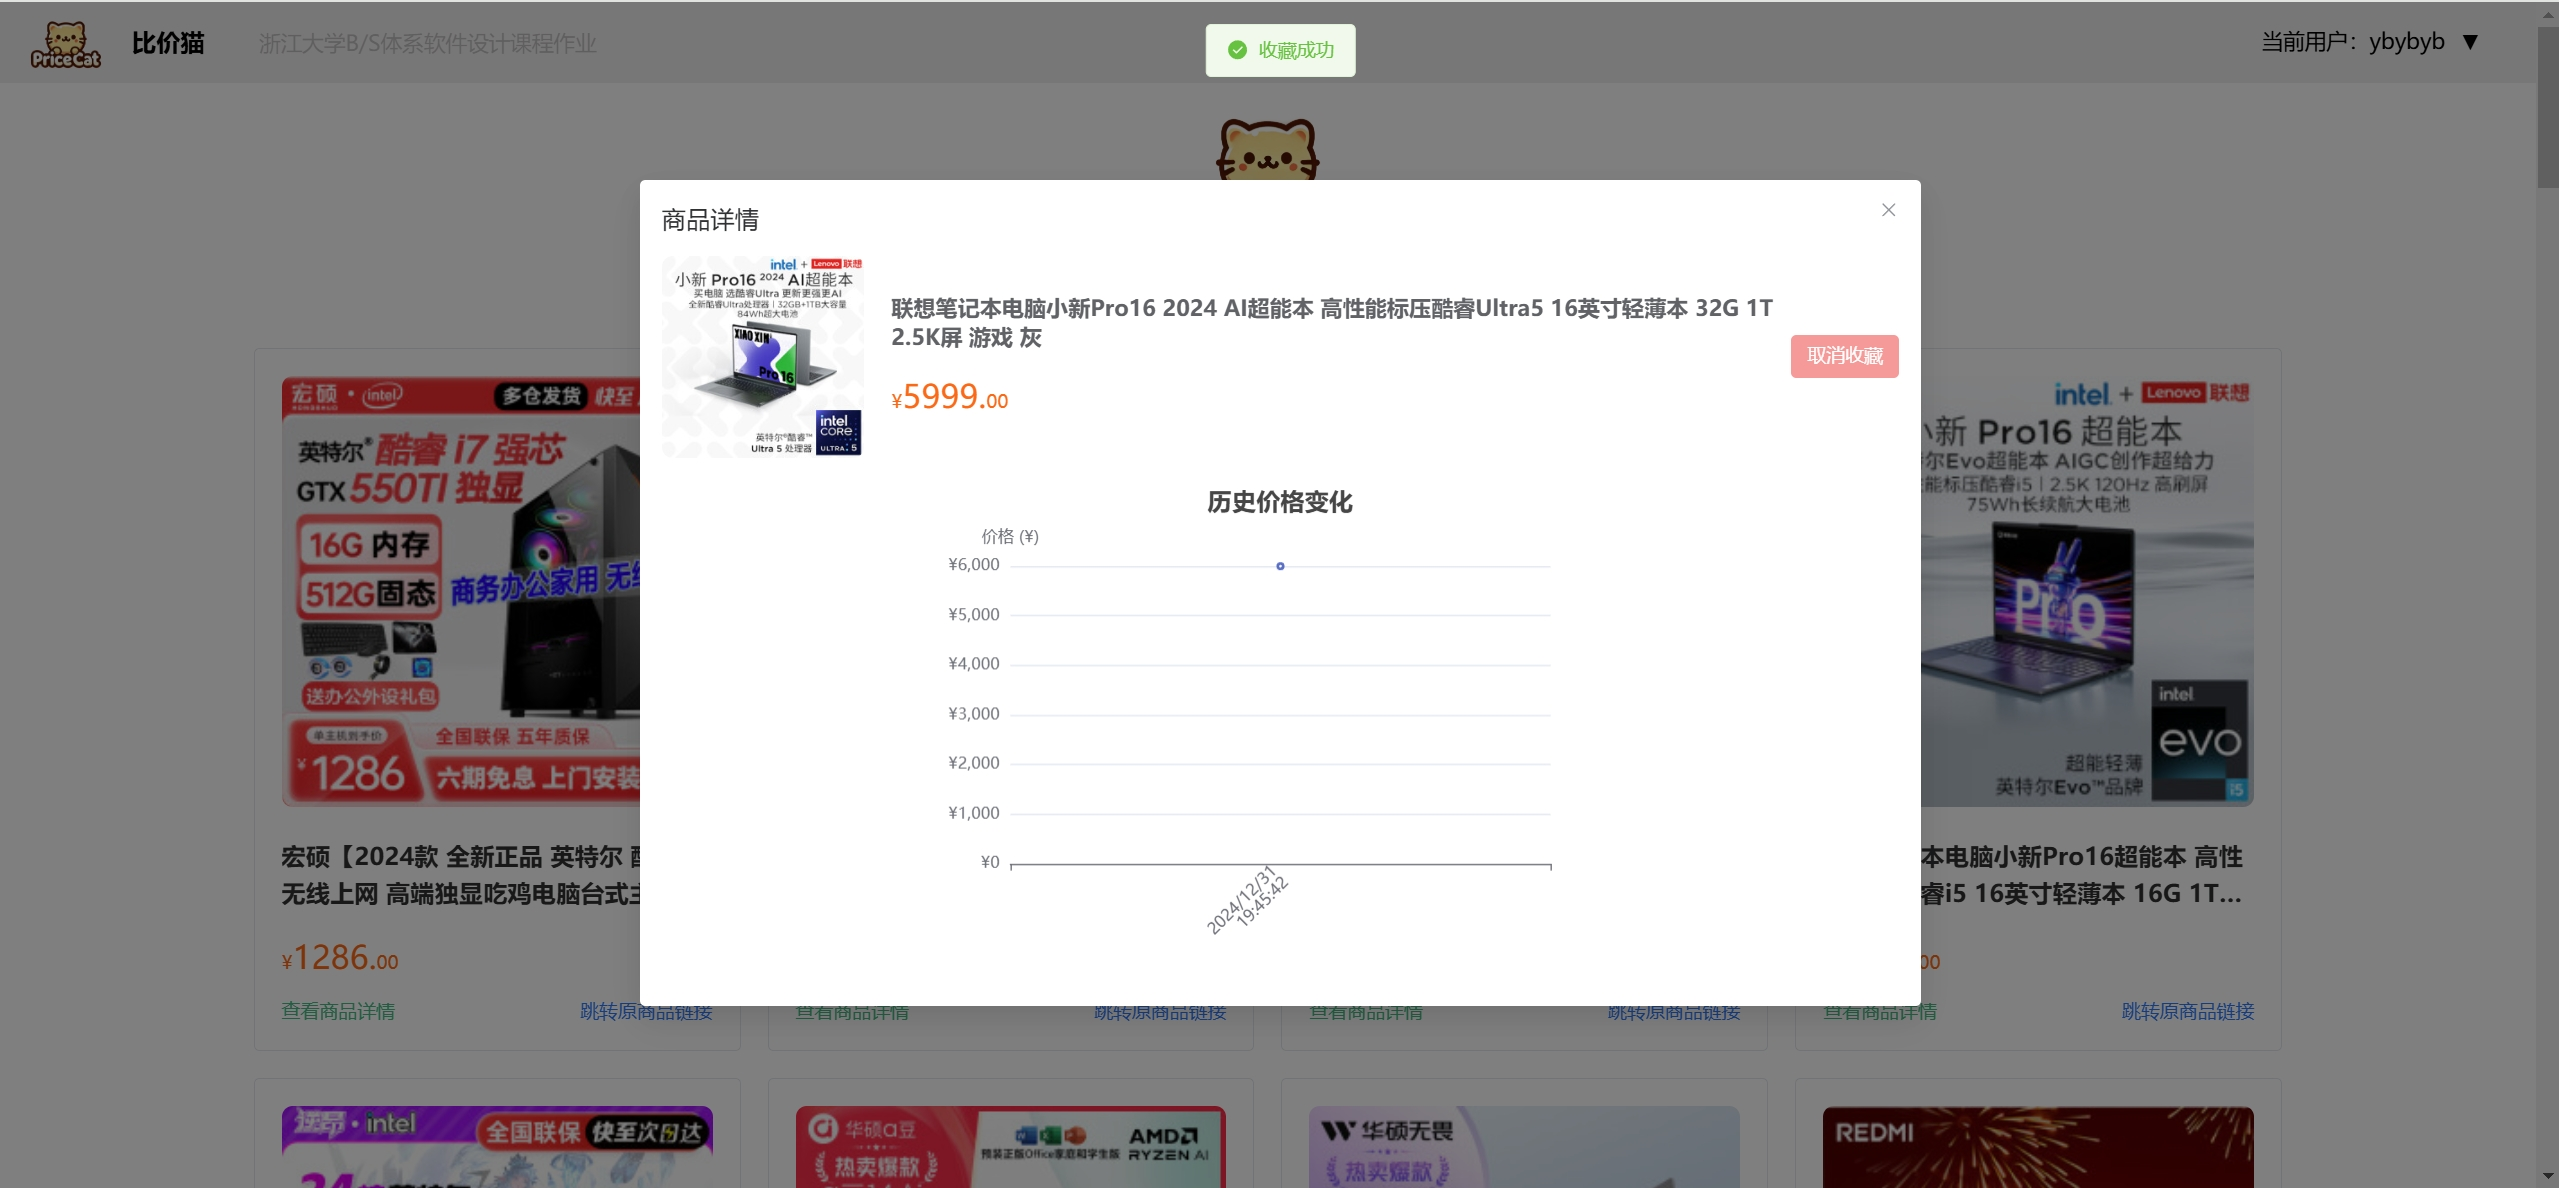
\includegraphics[width=1\textwidth]{./picture/商品收藏1.png}
\end{figure}

点击我的收藏，可以查看收藏的商品。
\begin{figure}[H]
  \centering
  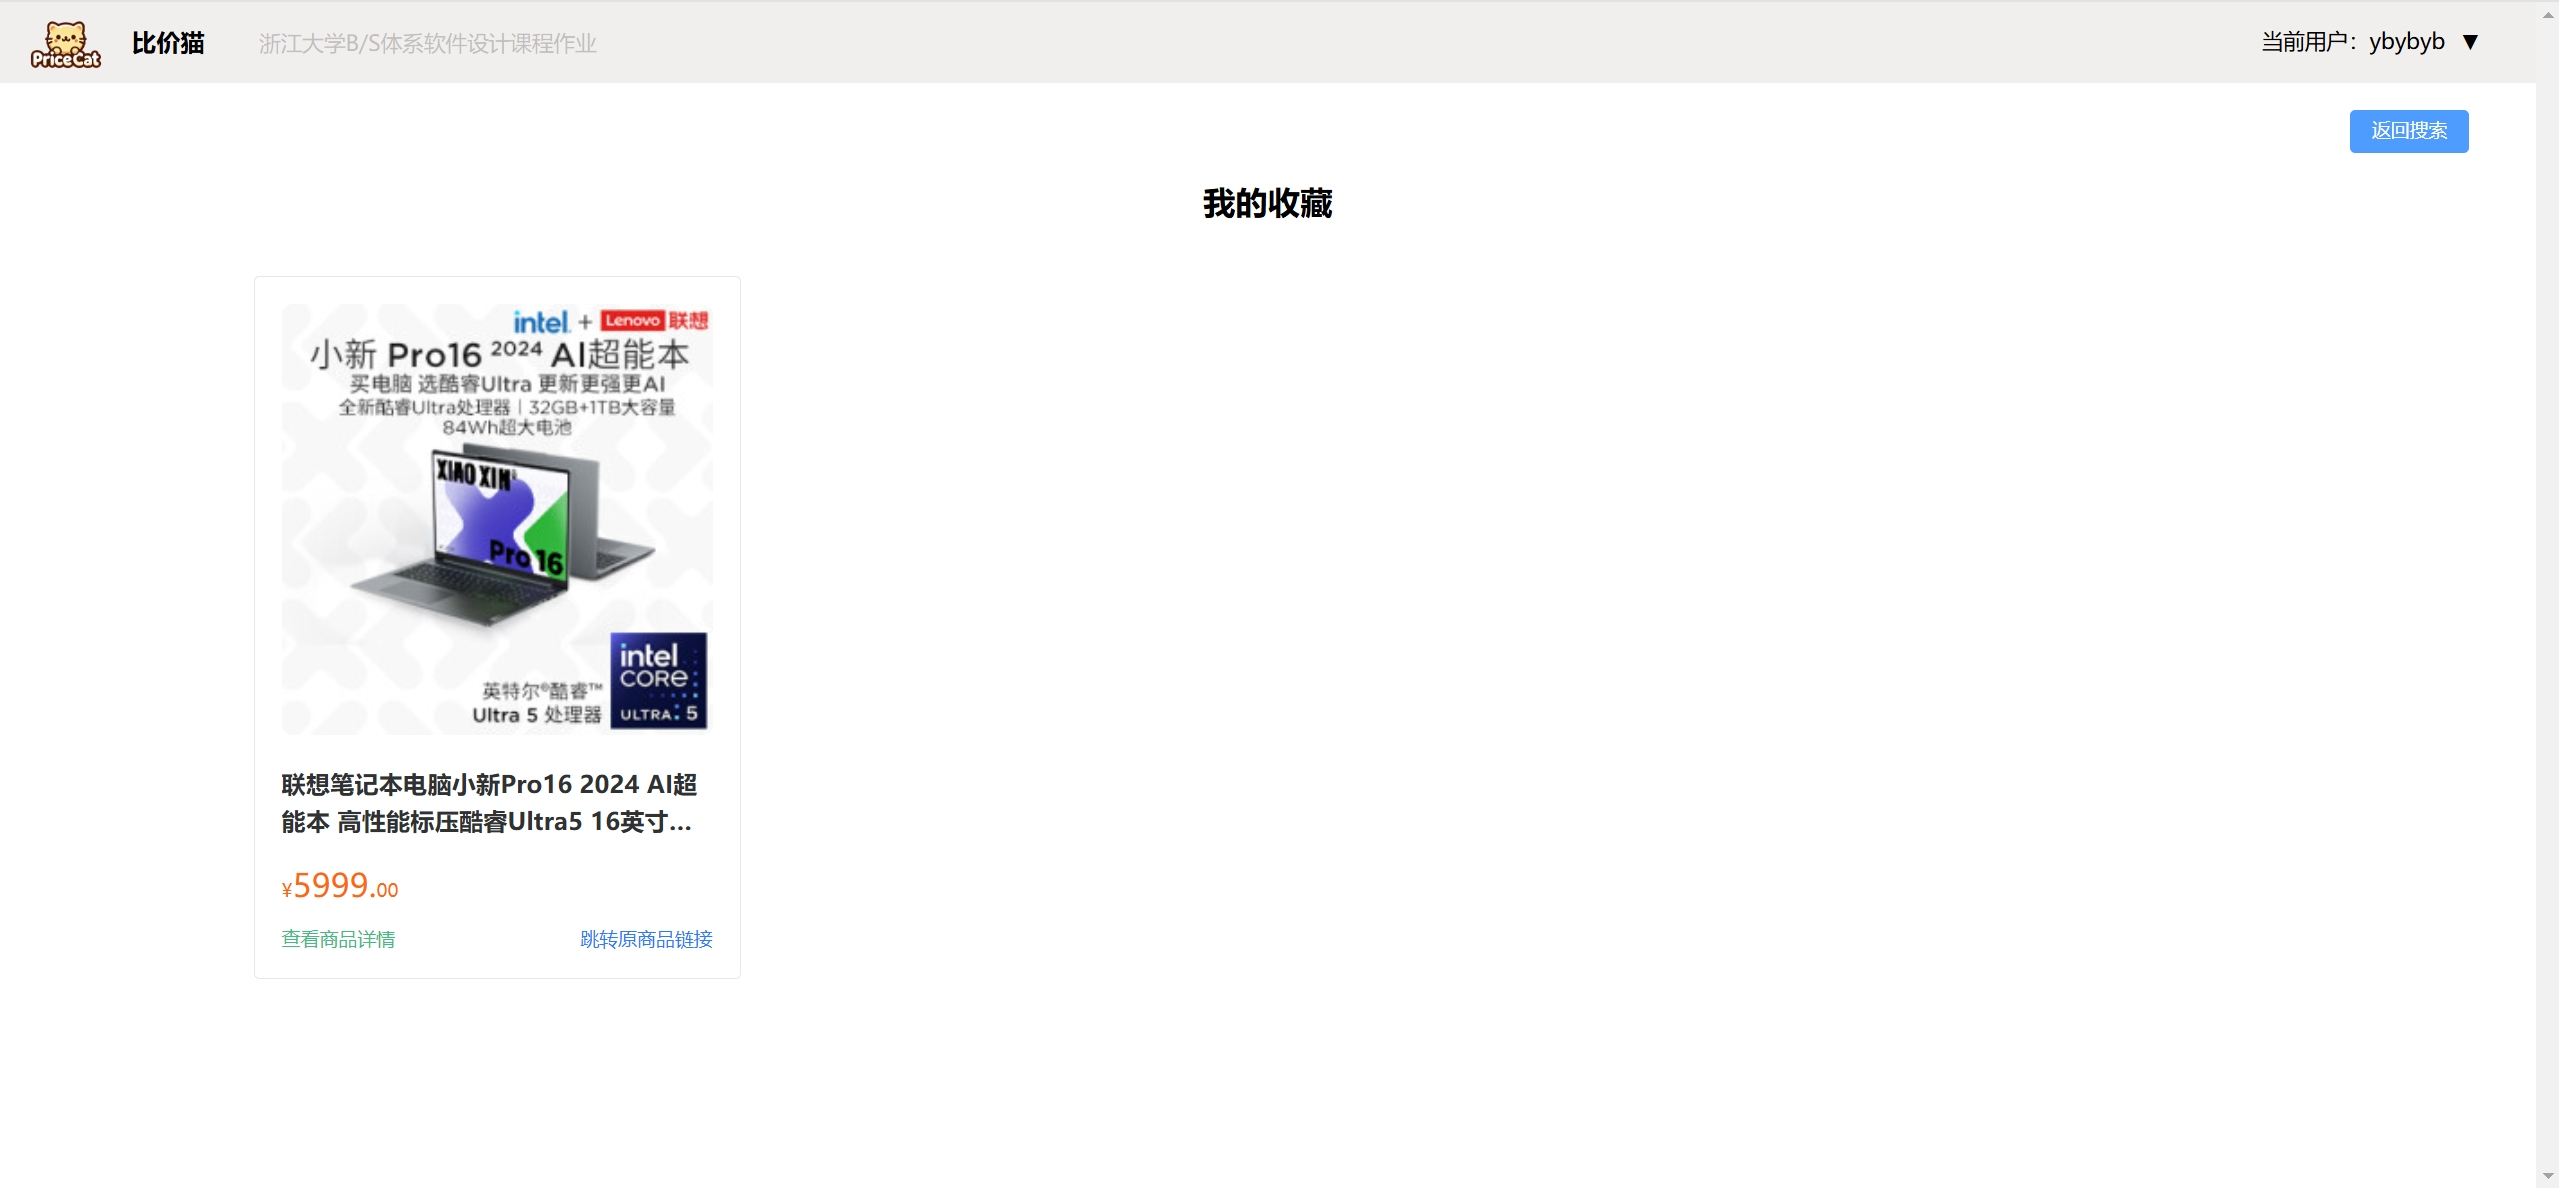
\includegraphics[width=1\textwidth]{./picture/商品收藏2.png}
\end{figure}

\subsubsection{降价提醒}
当商品价格下降时，可以收到降价提醒邮件。
\begin{figure}[H]
  \centering
  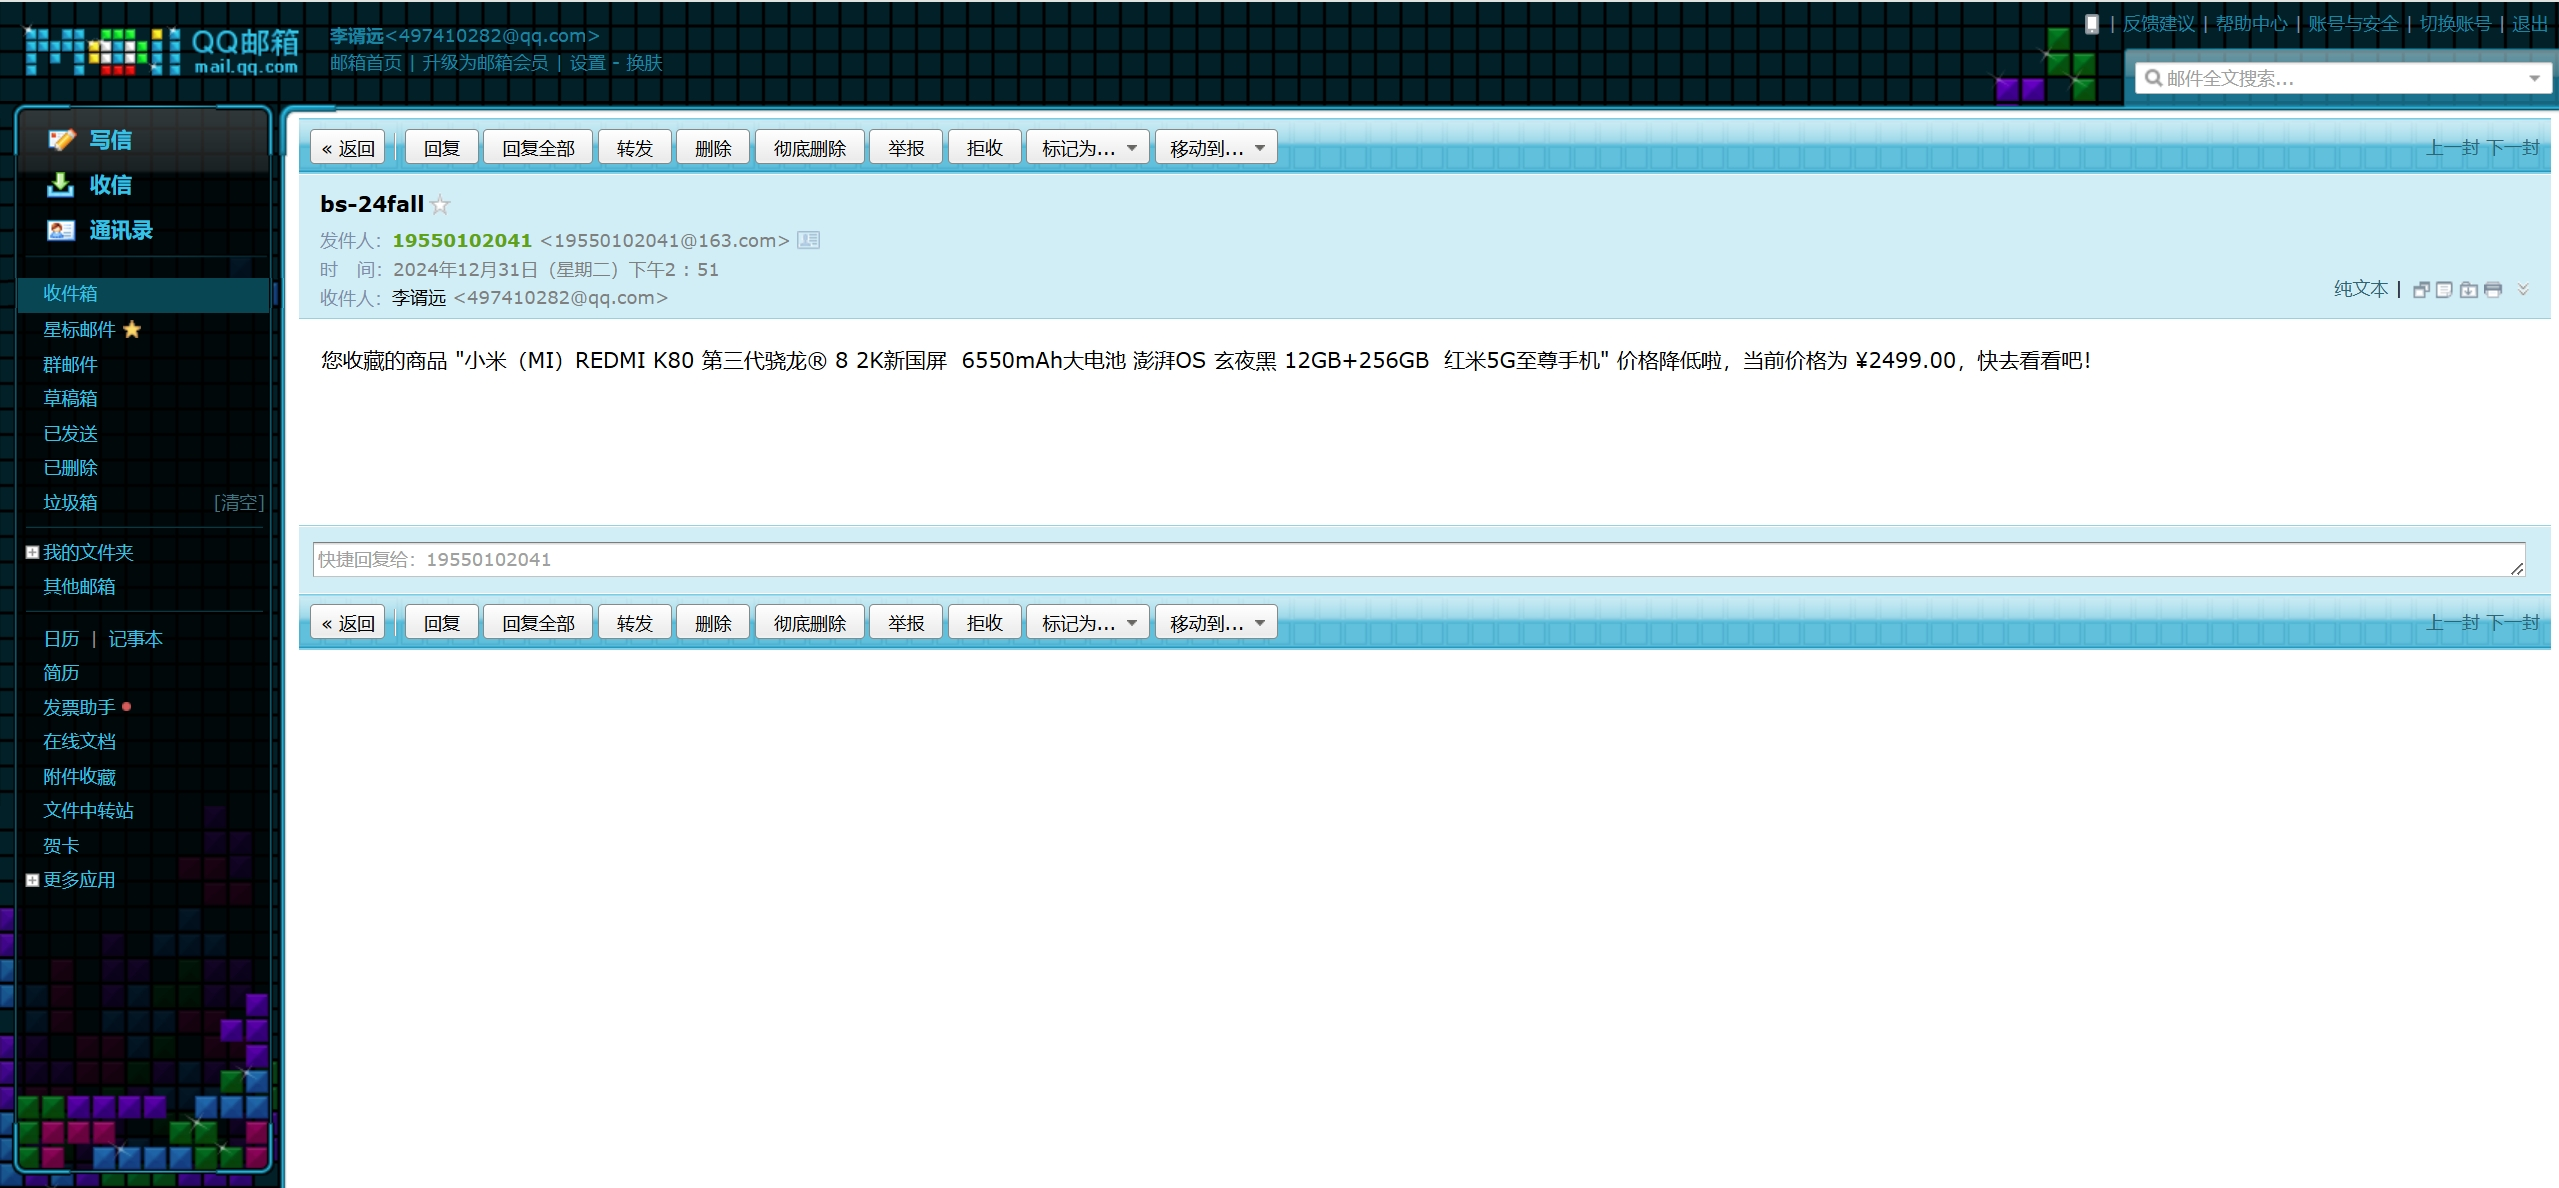
\includegraphics[width=1\textwidth]{./picture/降价提醒.png}
\end{figure}

\subsection{移动端适配}
访问移动端多个页面，均能正常显示。
\begin{figure}[H]
  \centering
  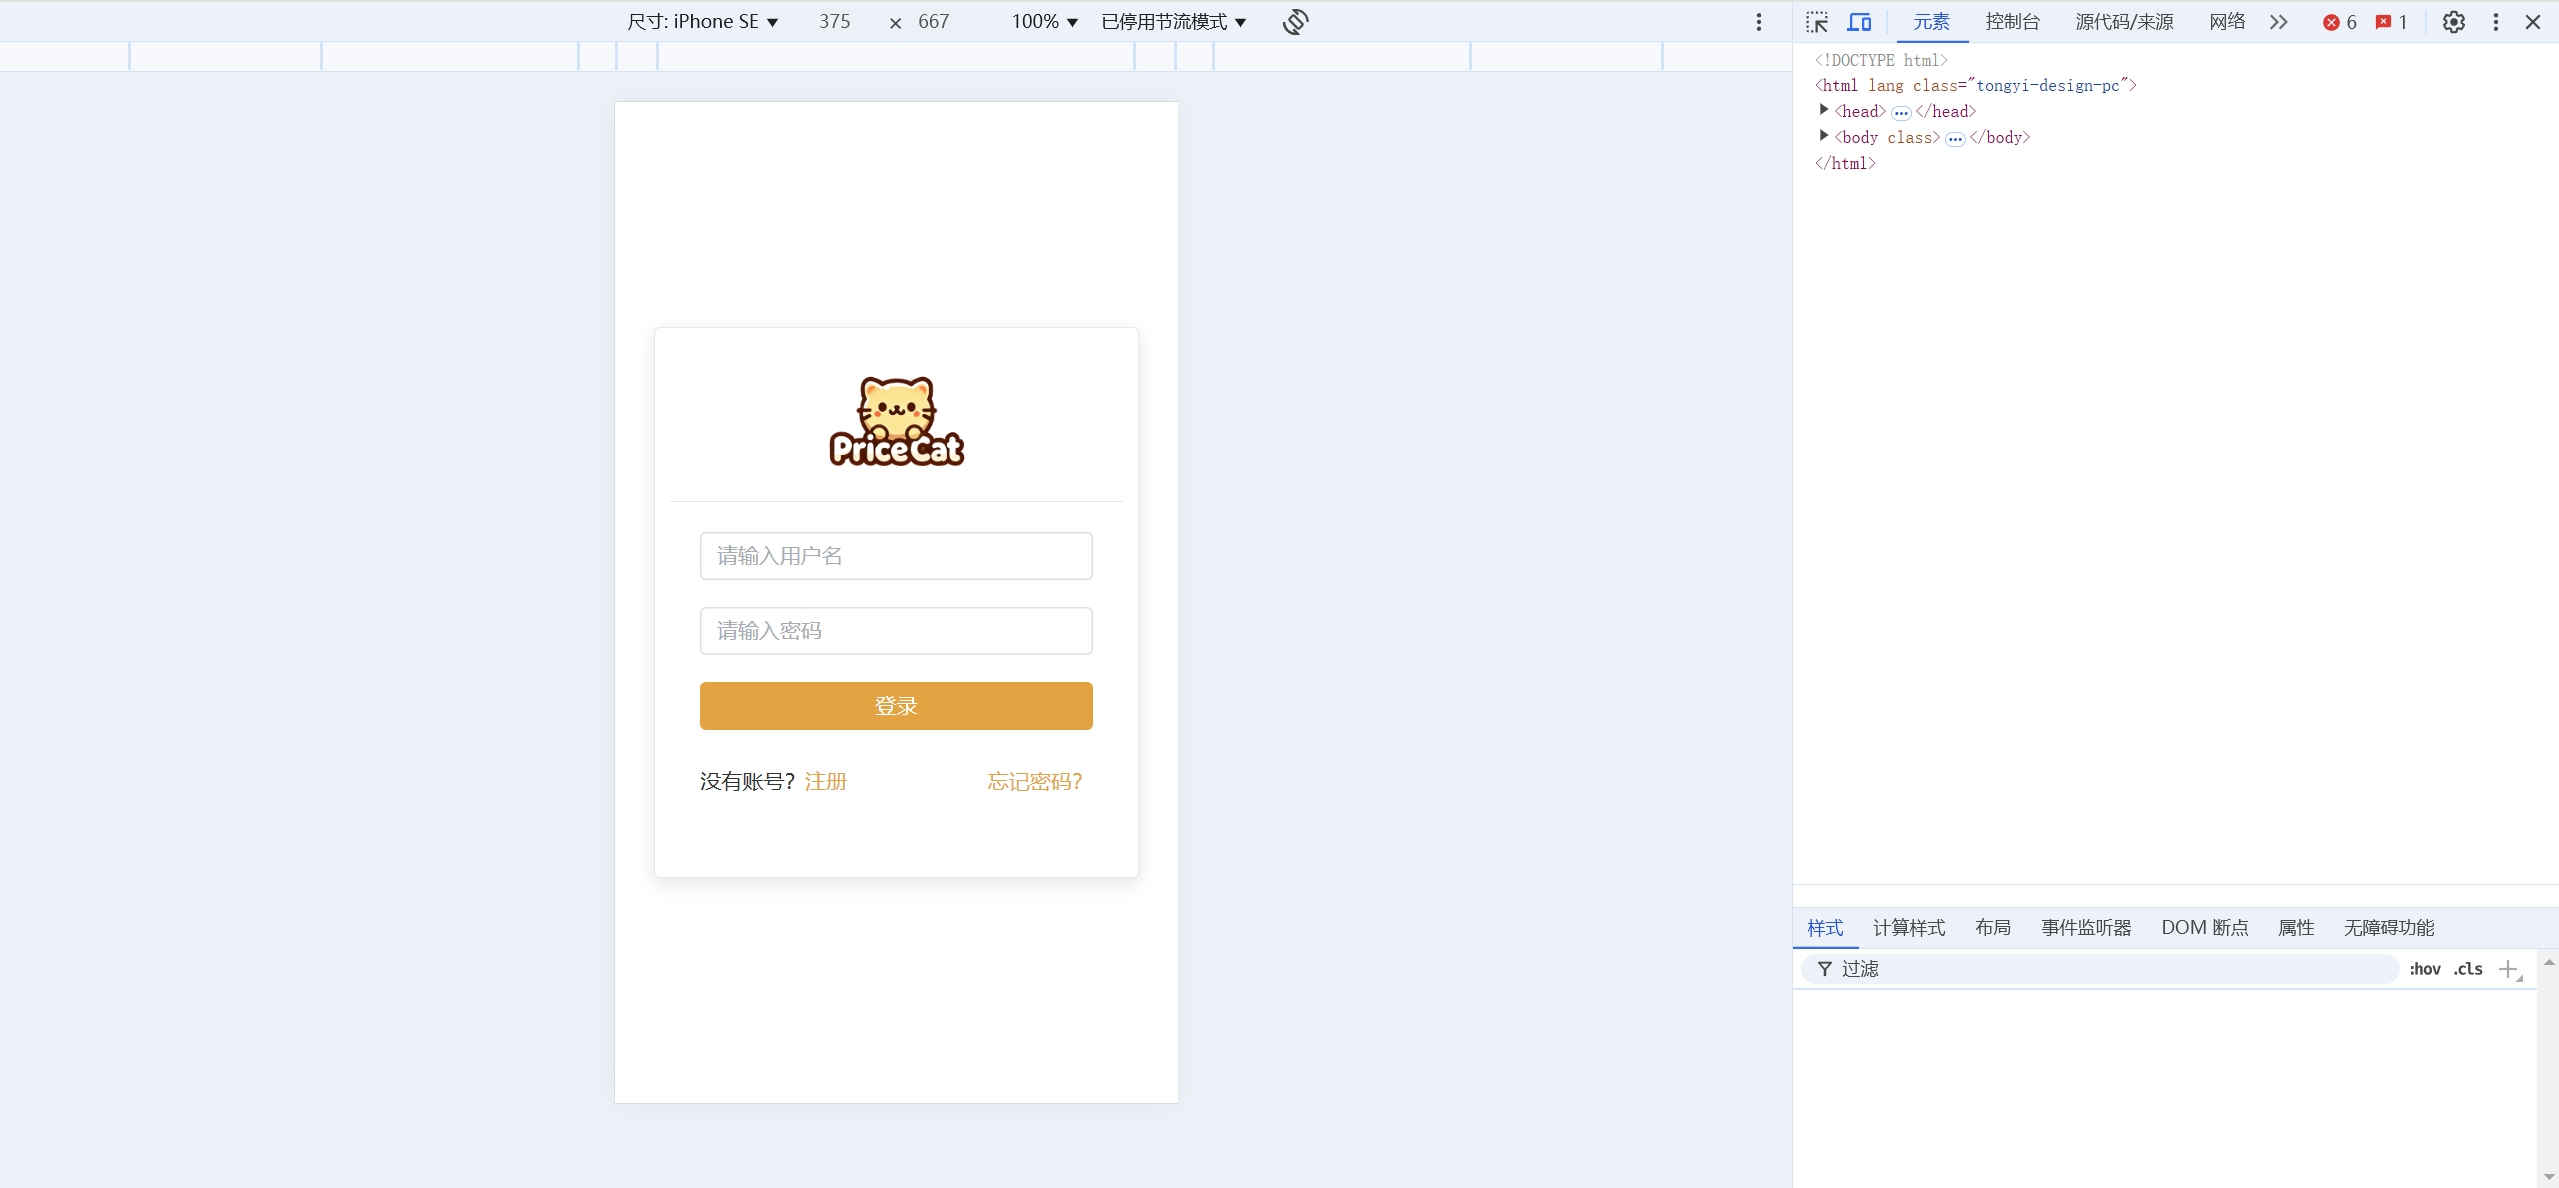
\includegraphics[width=1\textwidth]{./picture/移动端适配1.png}
\end{figure}

\begin{figure}[H]
  \centering
  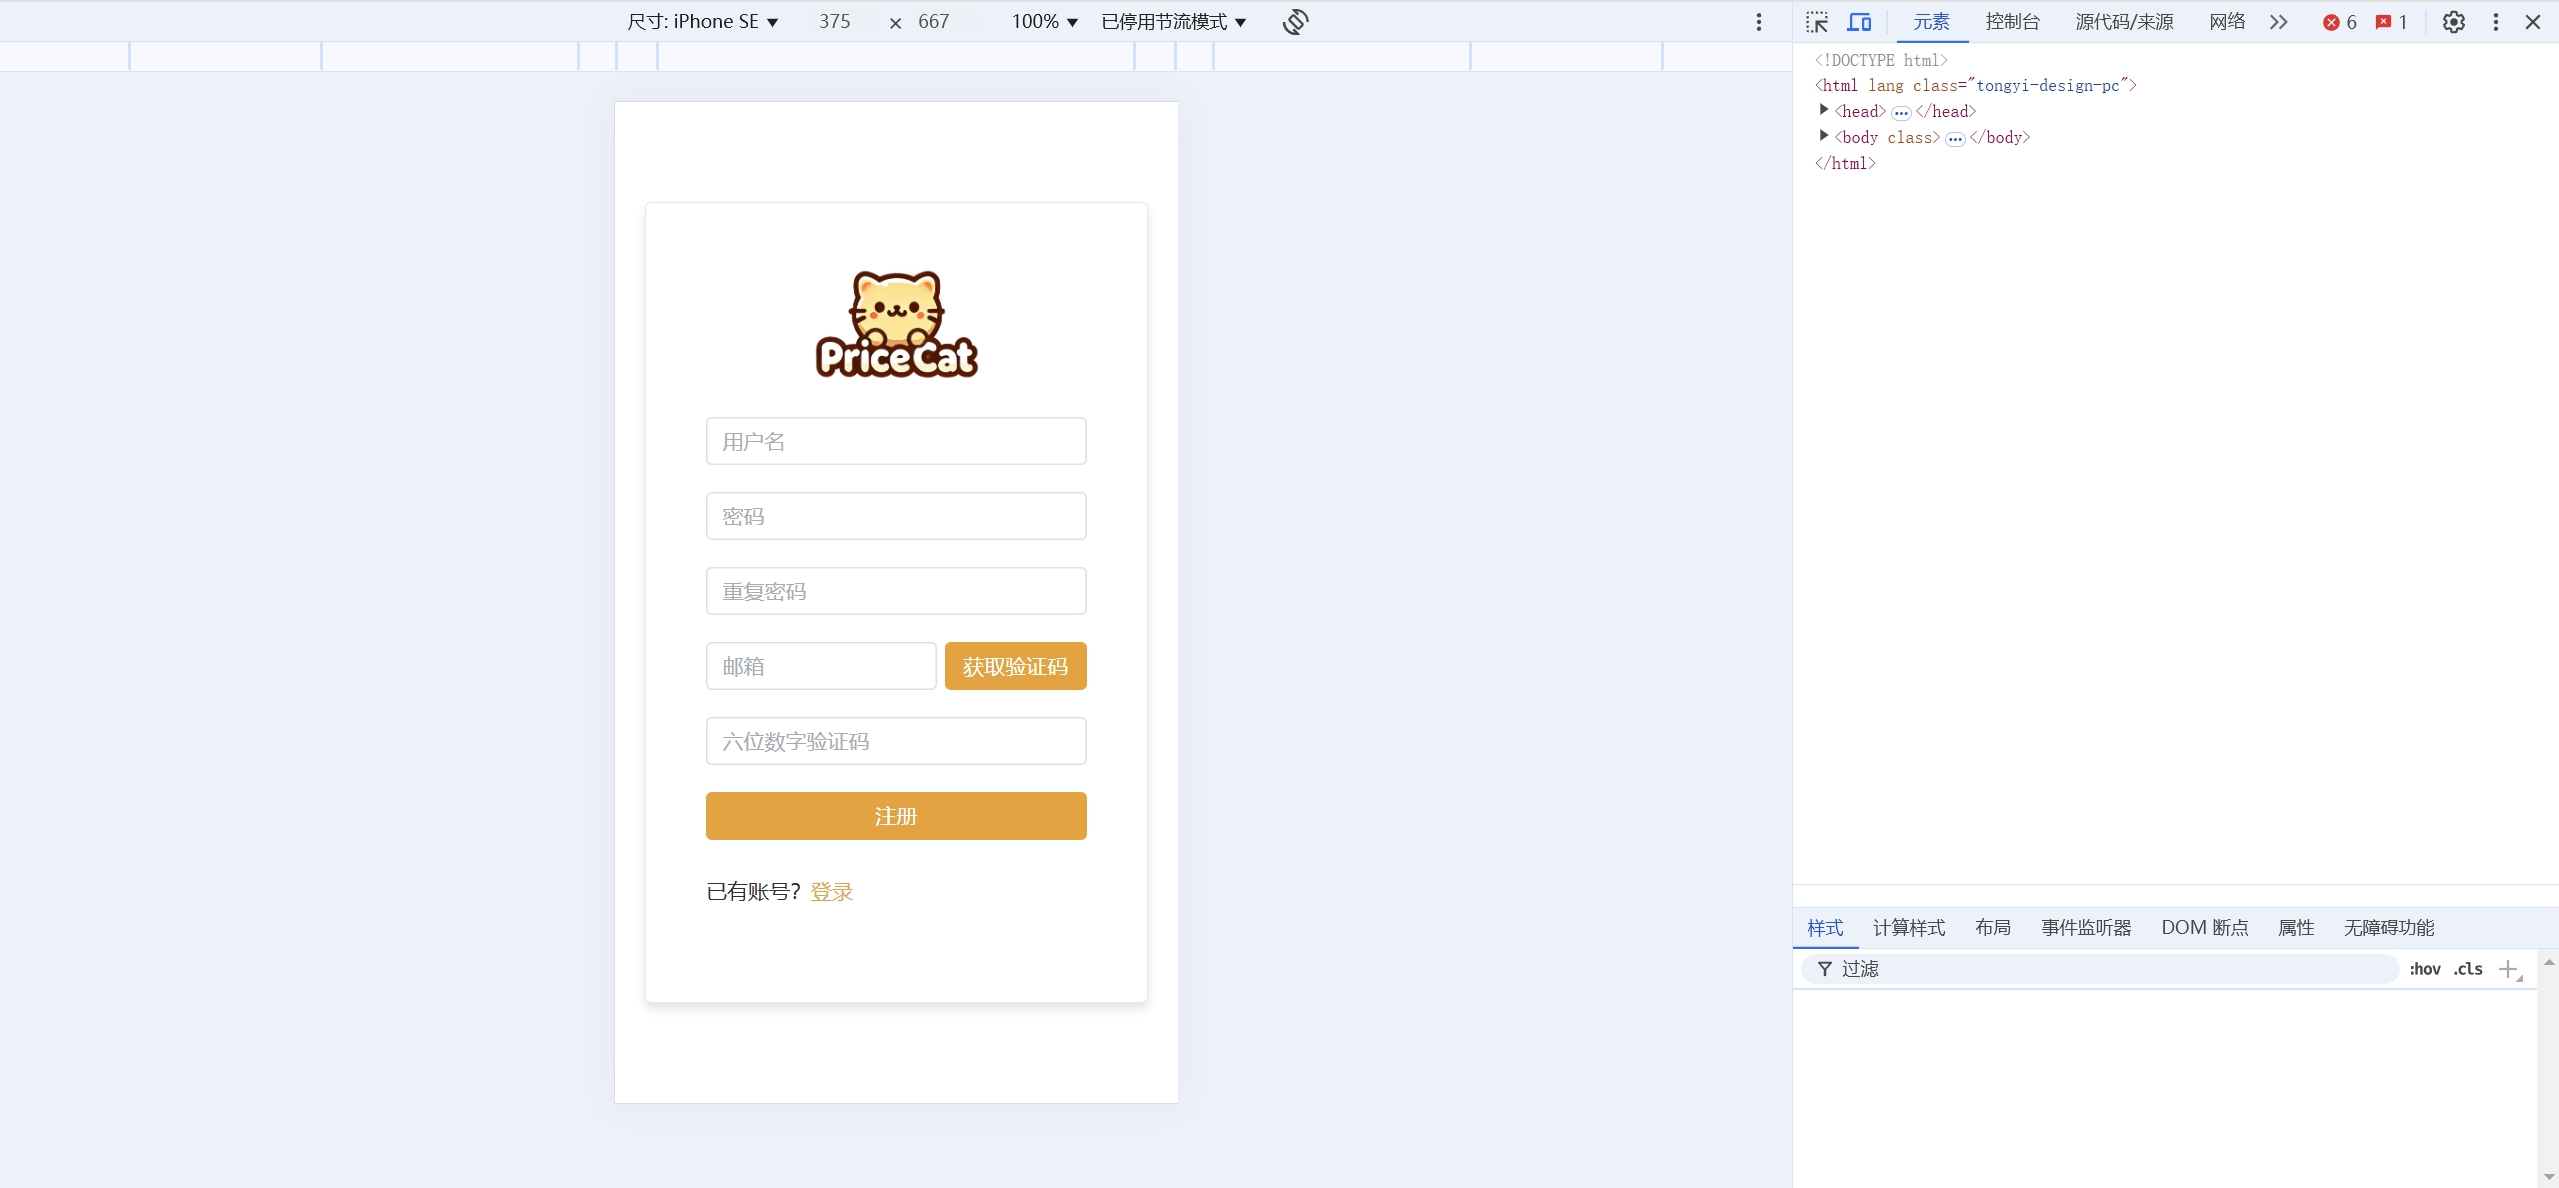
\includegraphics[width=1\textwidth]{./picture/移动端适配2.png}
\end{figure}

\begin{figure}[H]
  \centering
  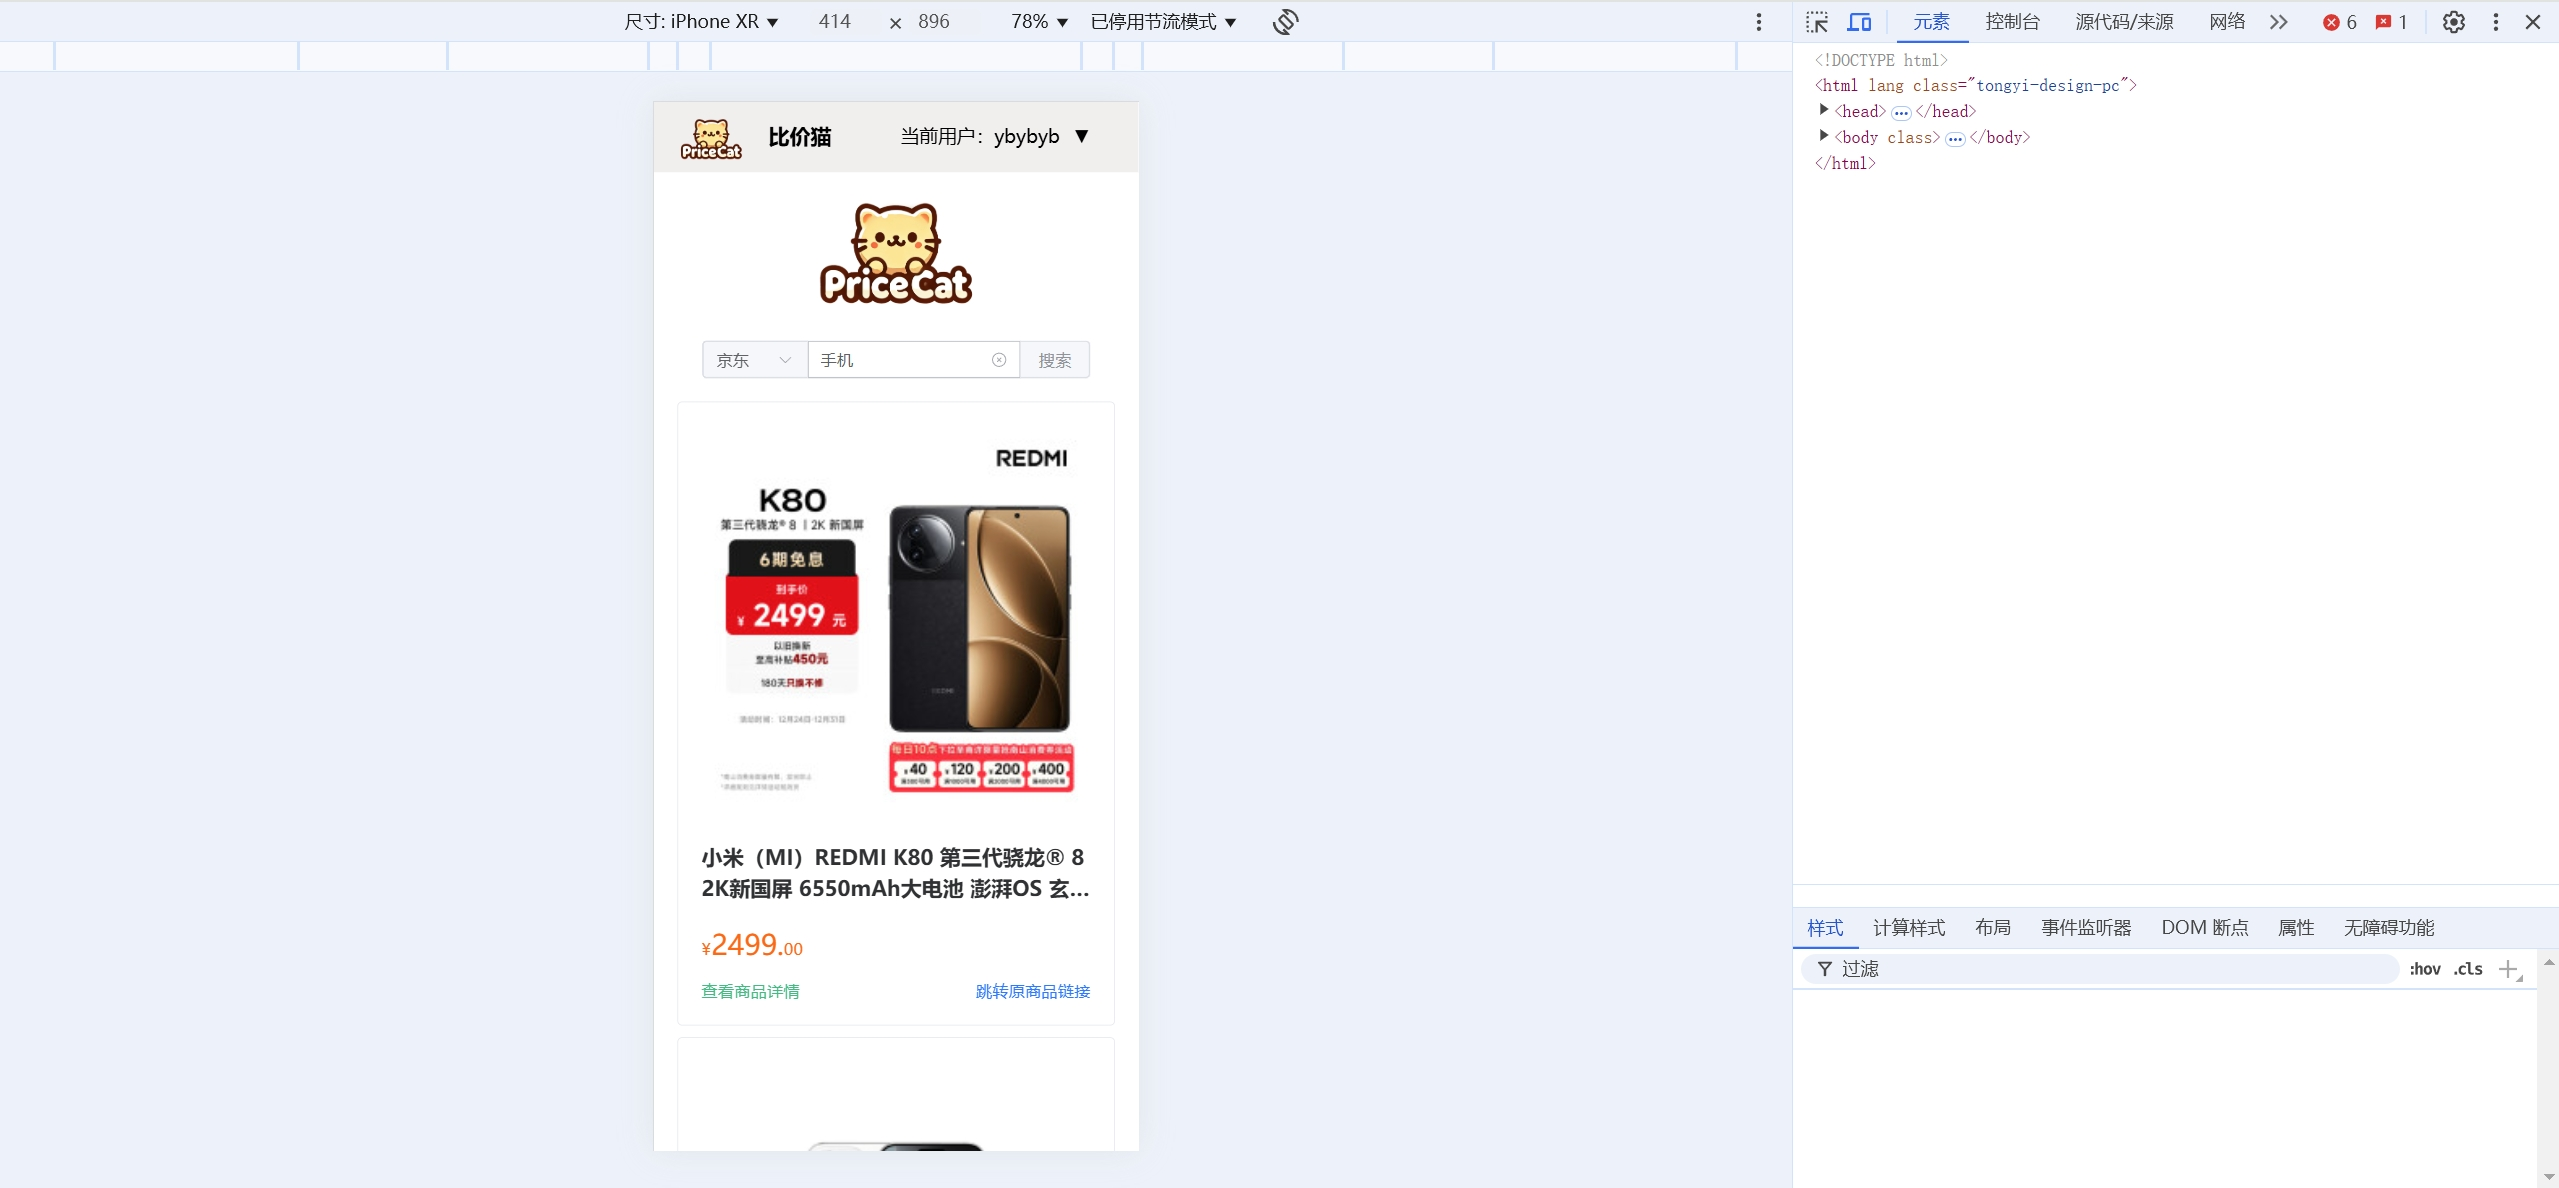
\includegraphics[width=1\textwidth]{./picture/移动端适配3.png}
\end{figure}

\begin{figure}[H]
  \centering
  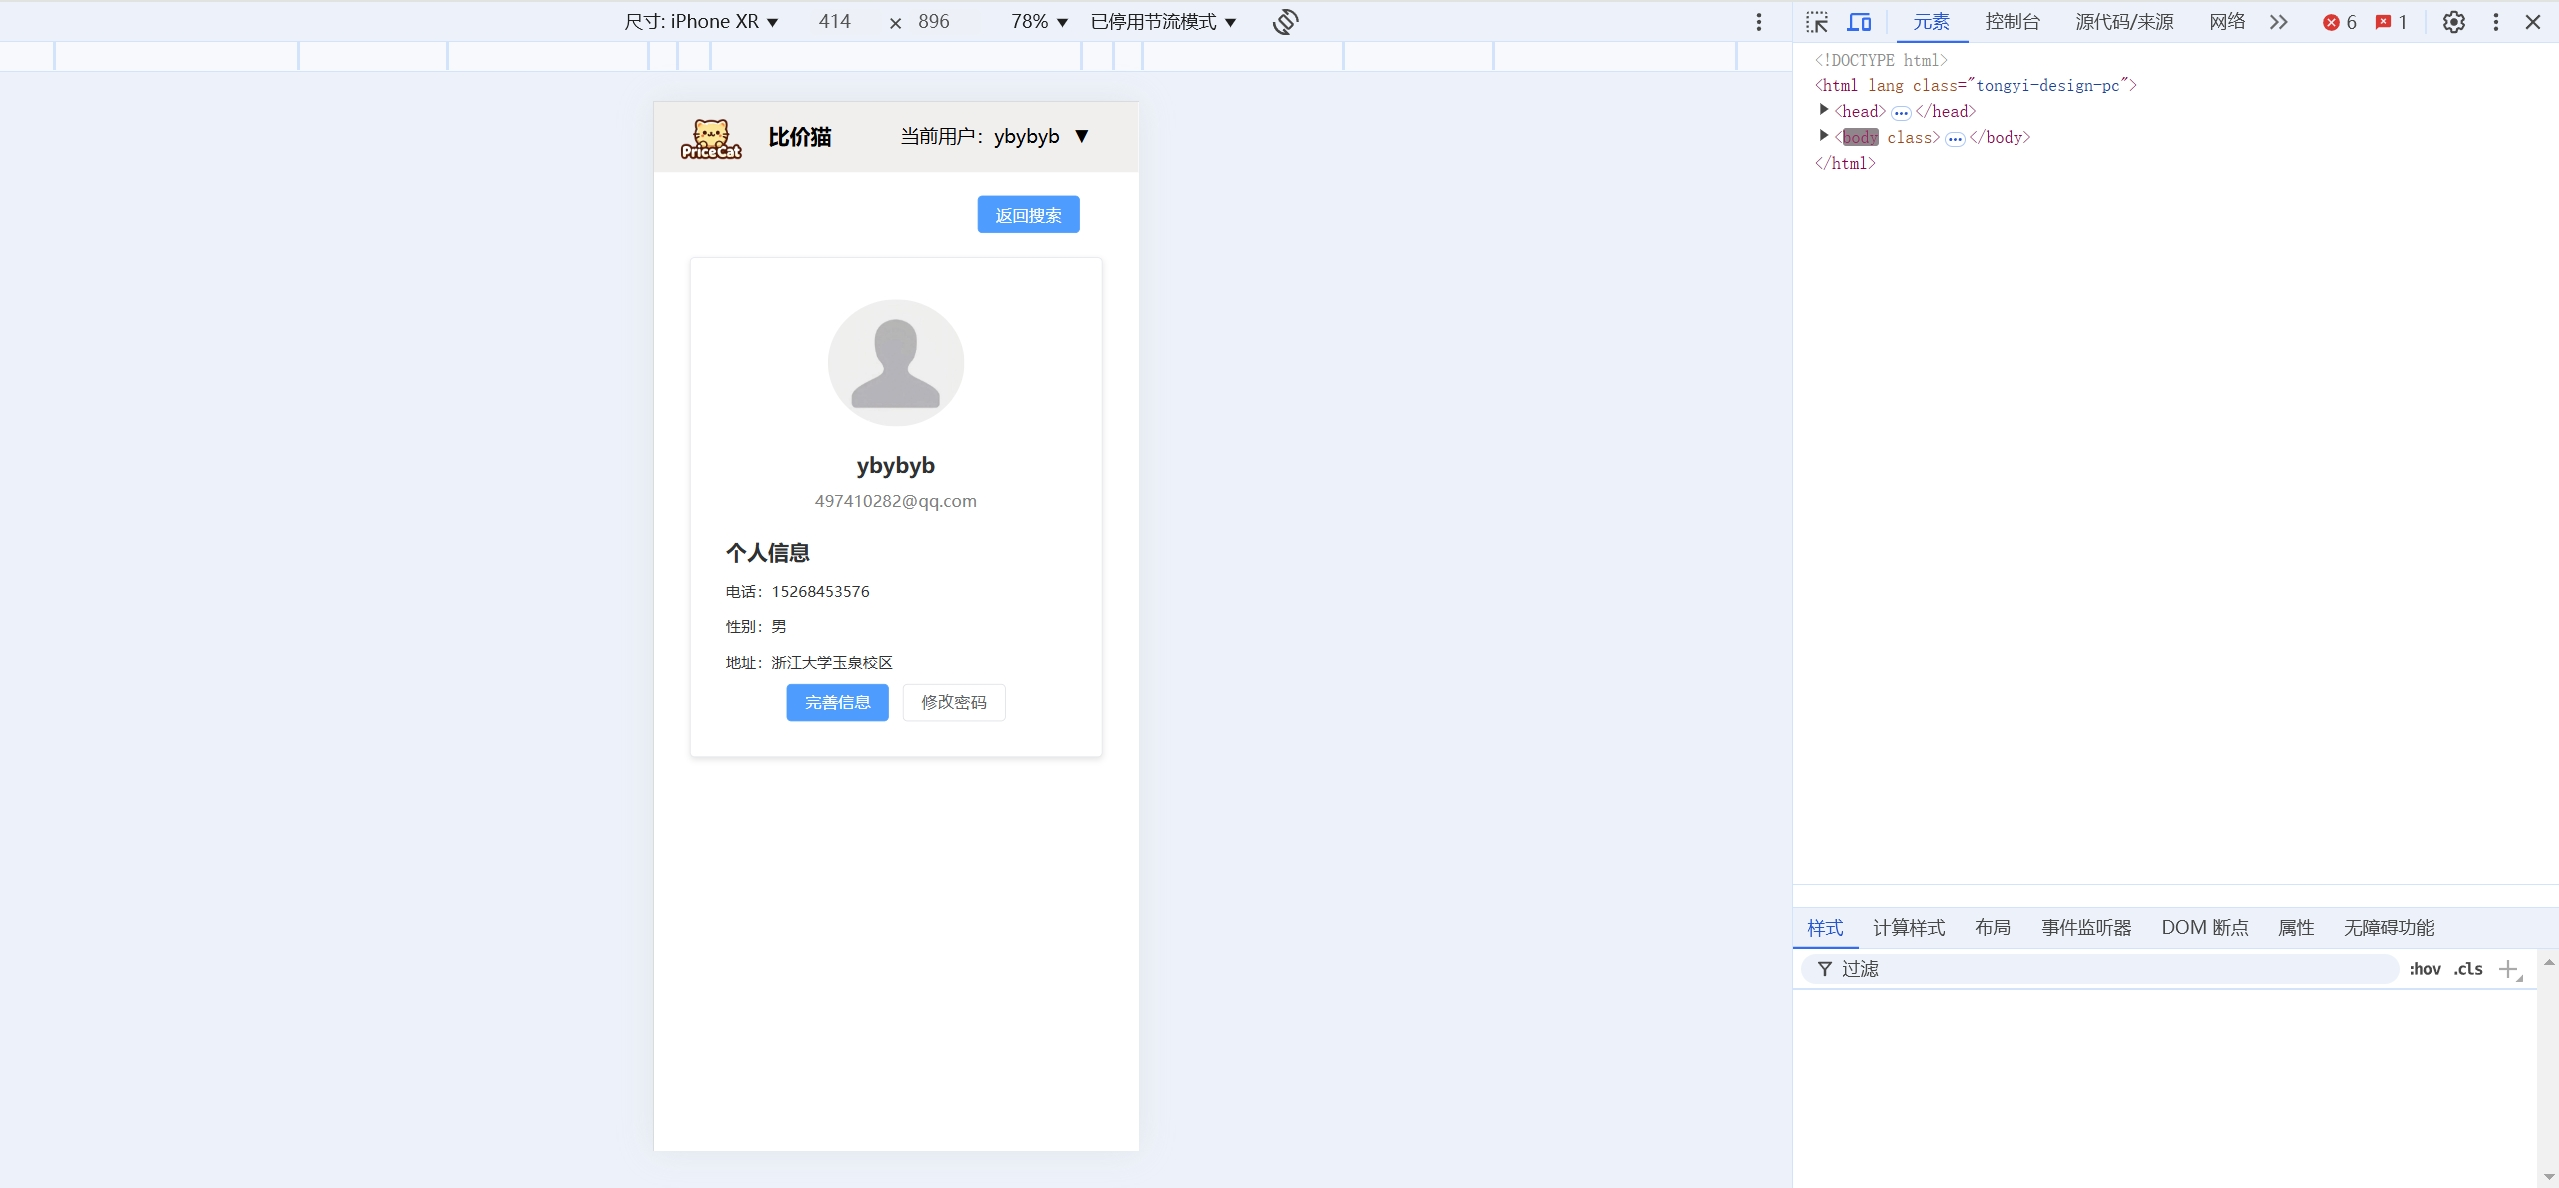
\includegraphics[width=1\textwidth]{./picture/移动端适配4.png}
\end{figure}

\section{边界值测试}

\subsection{用户账户模块}

\subsubsection{用户注册}
输入不合法的用户名、密码、邮箱地址和验证码，任一不合法不能成功注册。
\begin{figure}[H]
  \centering
  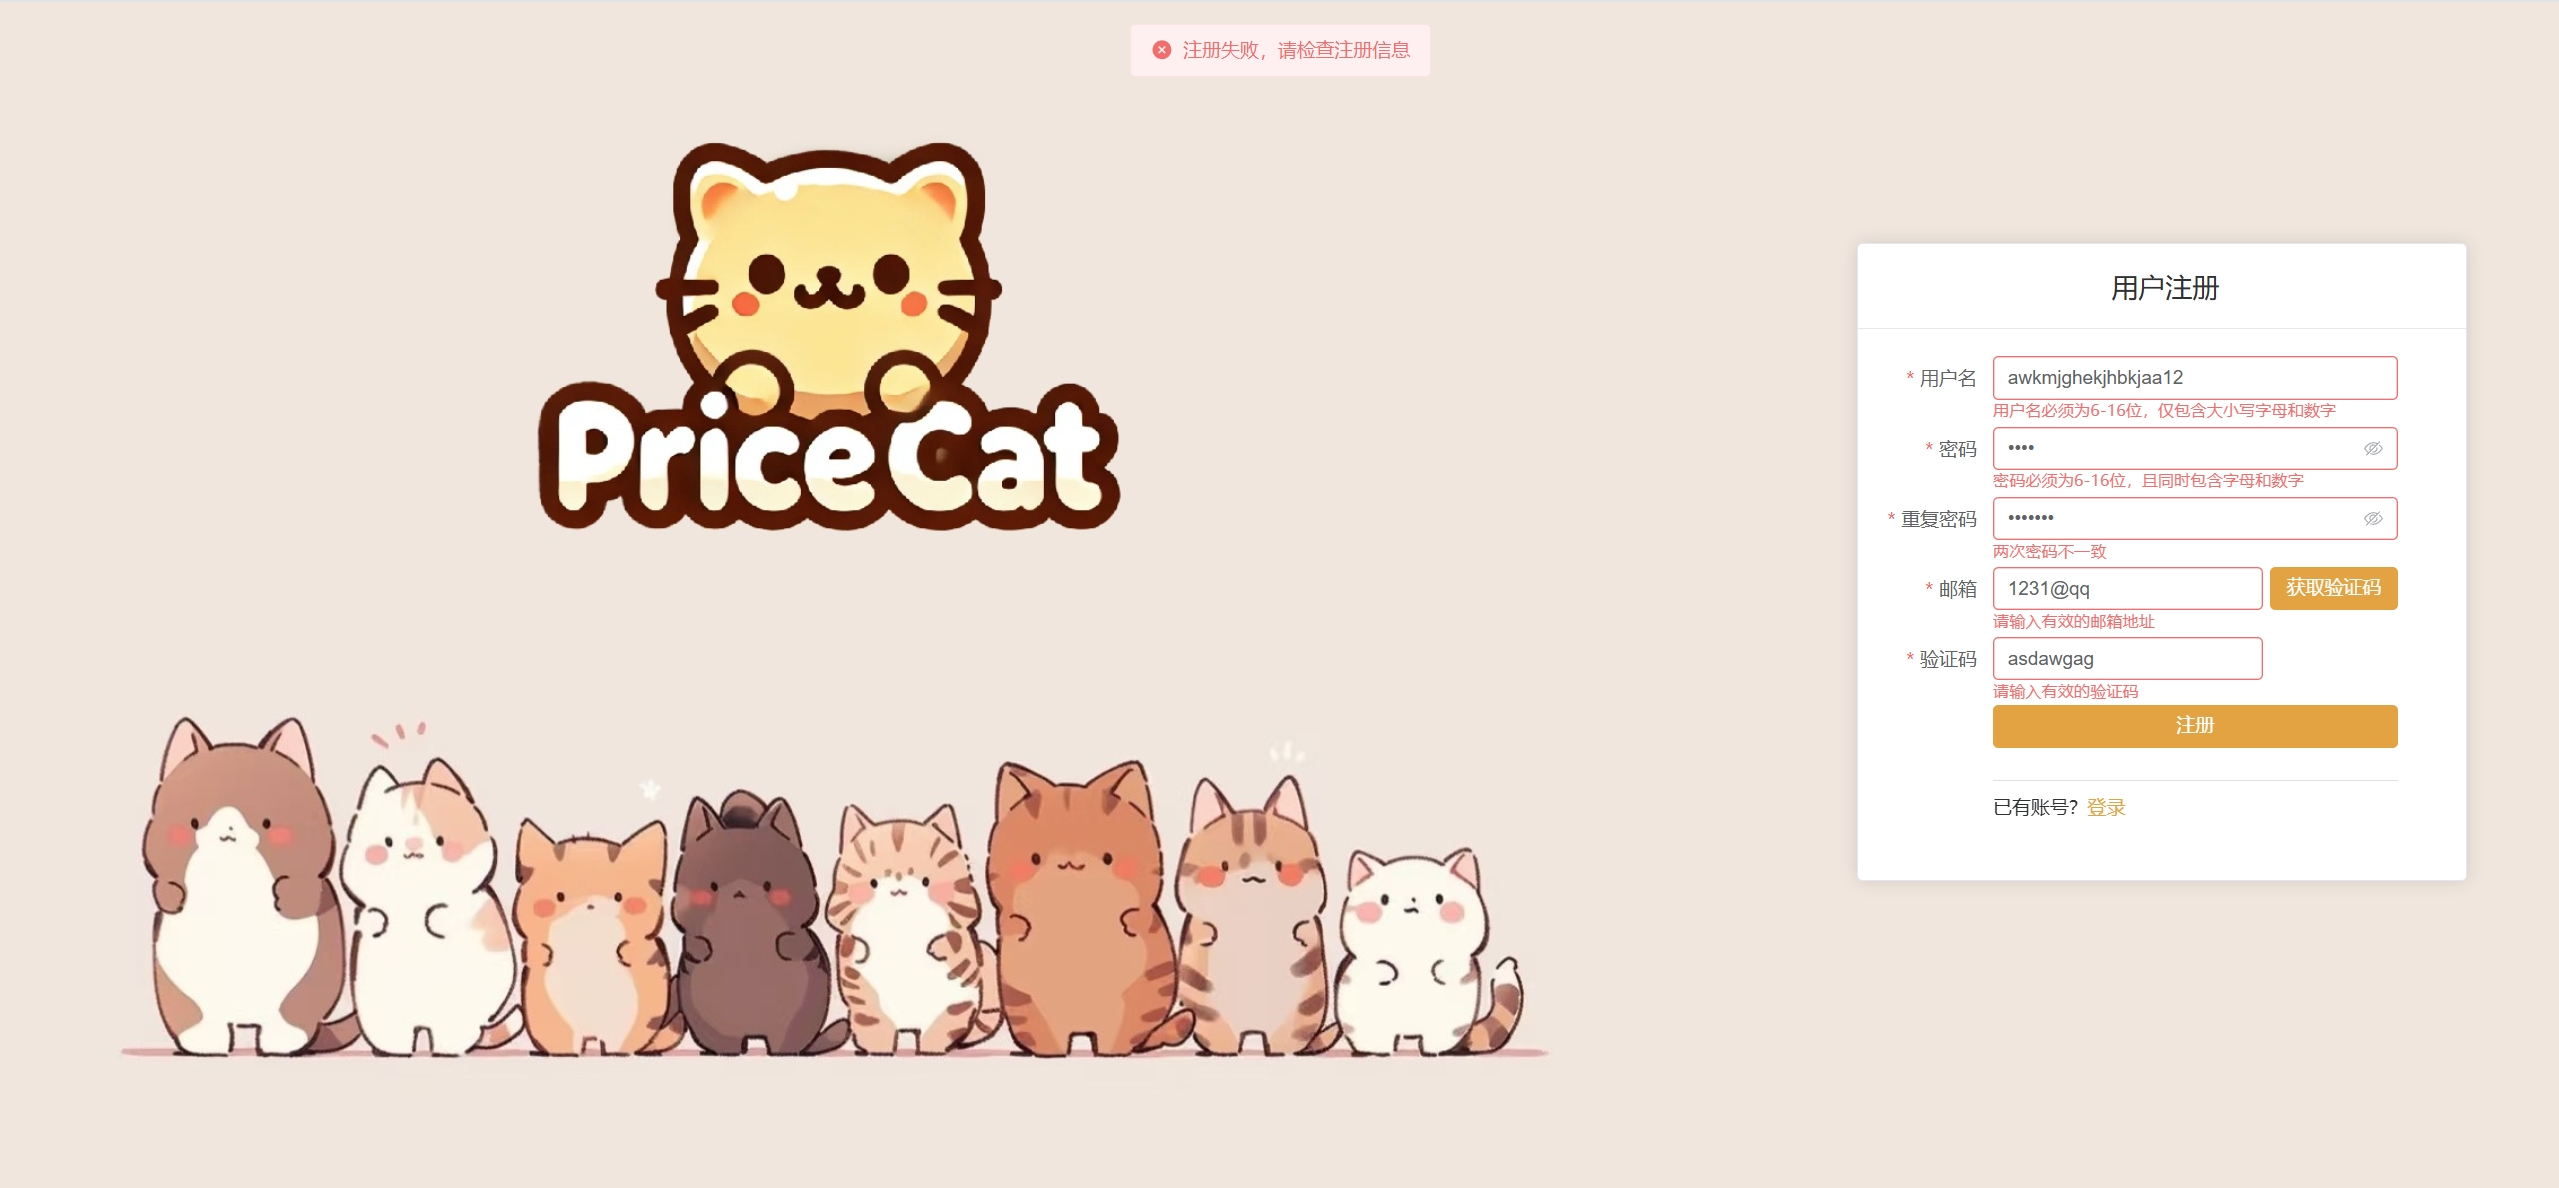
\includegraphics[width=1\textwidth]{./picture/用户注册边界值.png}
\end{figure}

\subsubsection{用户登录}
输入不合法的用户名和密码，不能成功登录。
\begin{figure}[H]
  \centering
  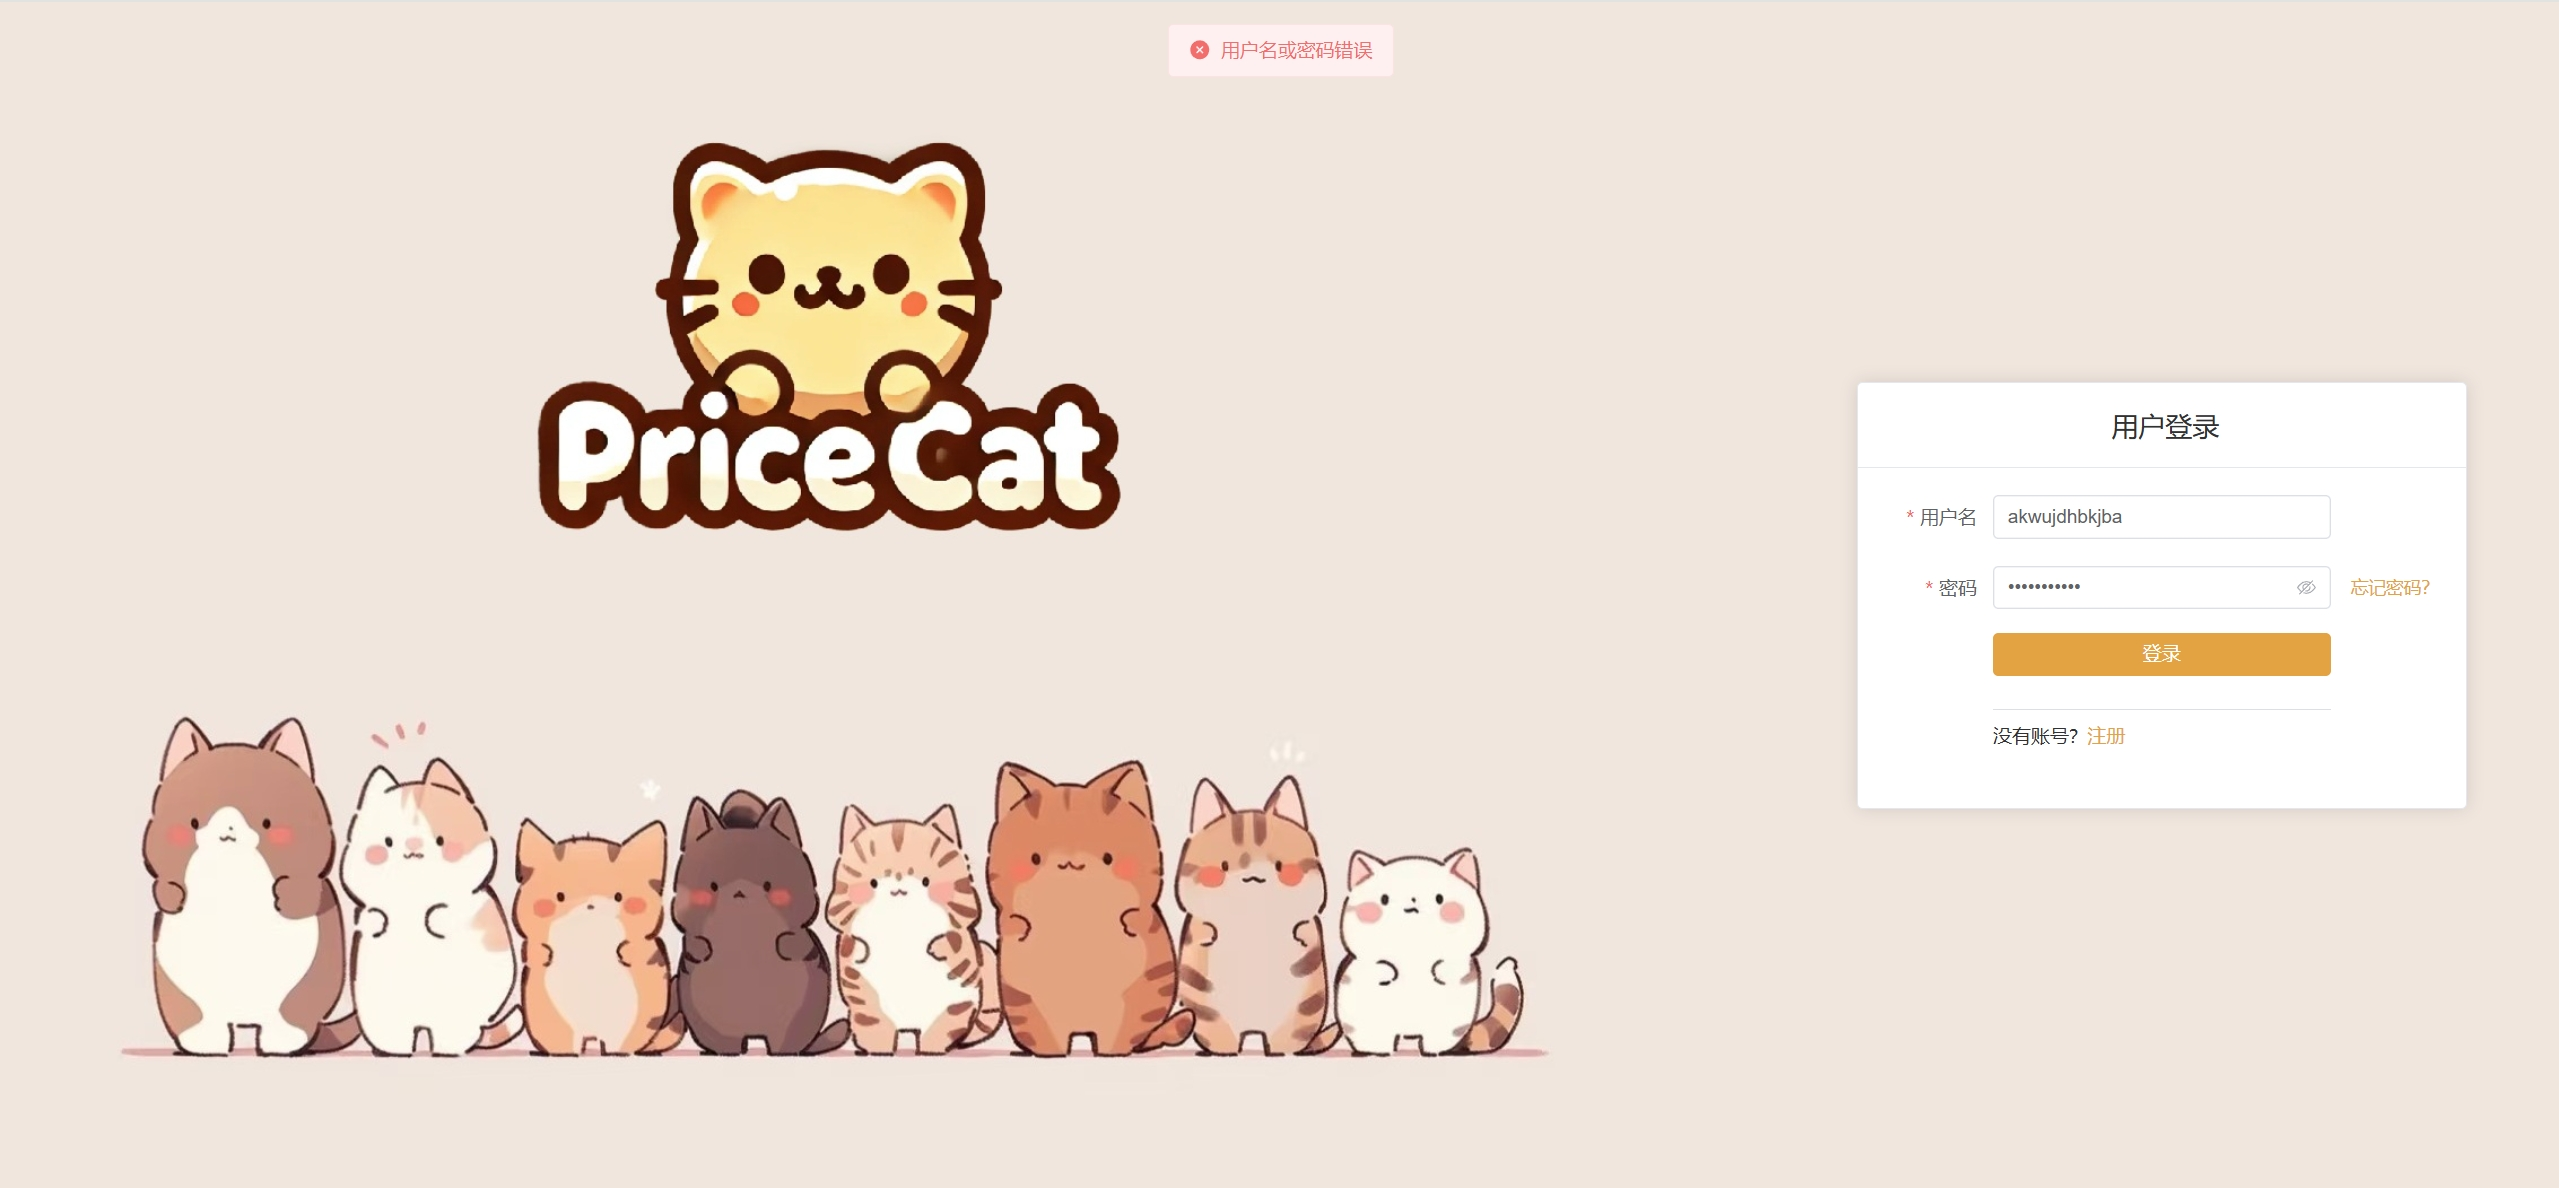
\includegraphics[width=1\textwidth]{./picture/用户登录边界值.png}
\end{figure}

\subsection{商品模块}

\subsubsection{商品查询}
输入不合法的商品名称，不能查询到商品信息。
\begin{figure}[H]
  \centering
  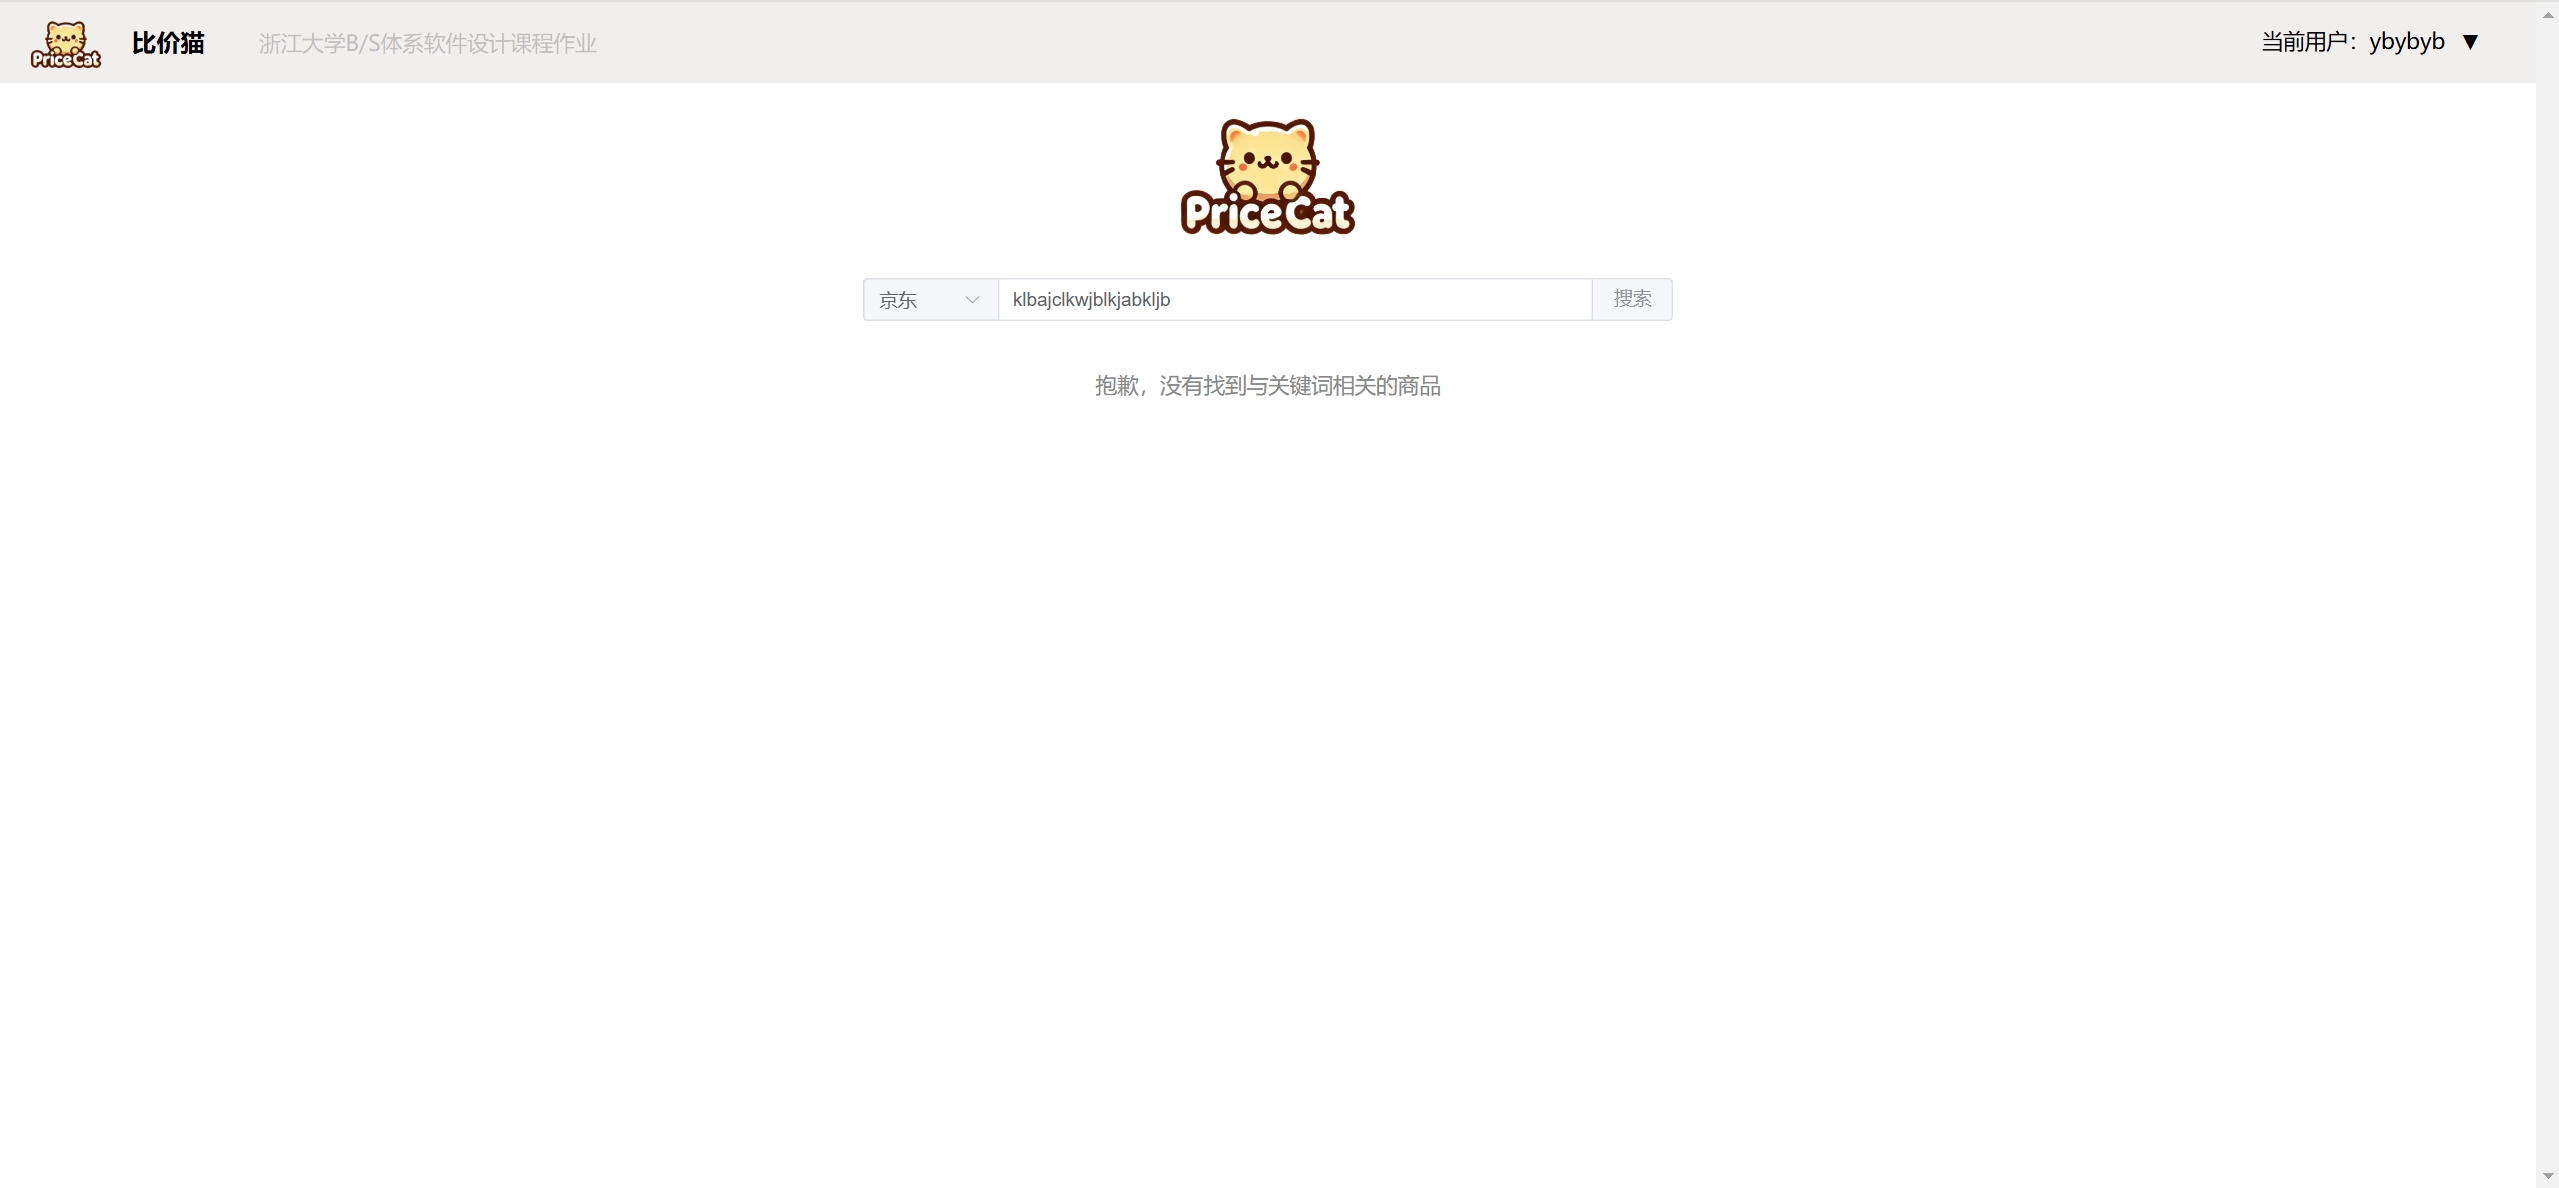
\includegraphics[width=1\textwidth]{./picture/商品查询边界值1.png}
\end{figure}

不输入商品名称，不能查询到商品信息。
\begin{figure}[H]
  \centering
  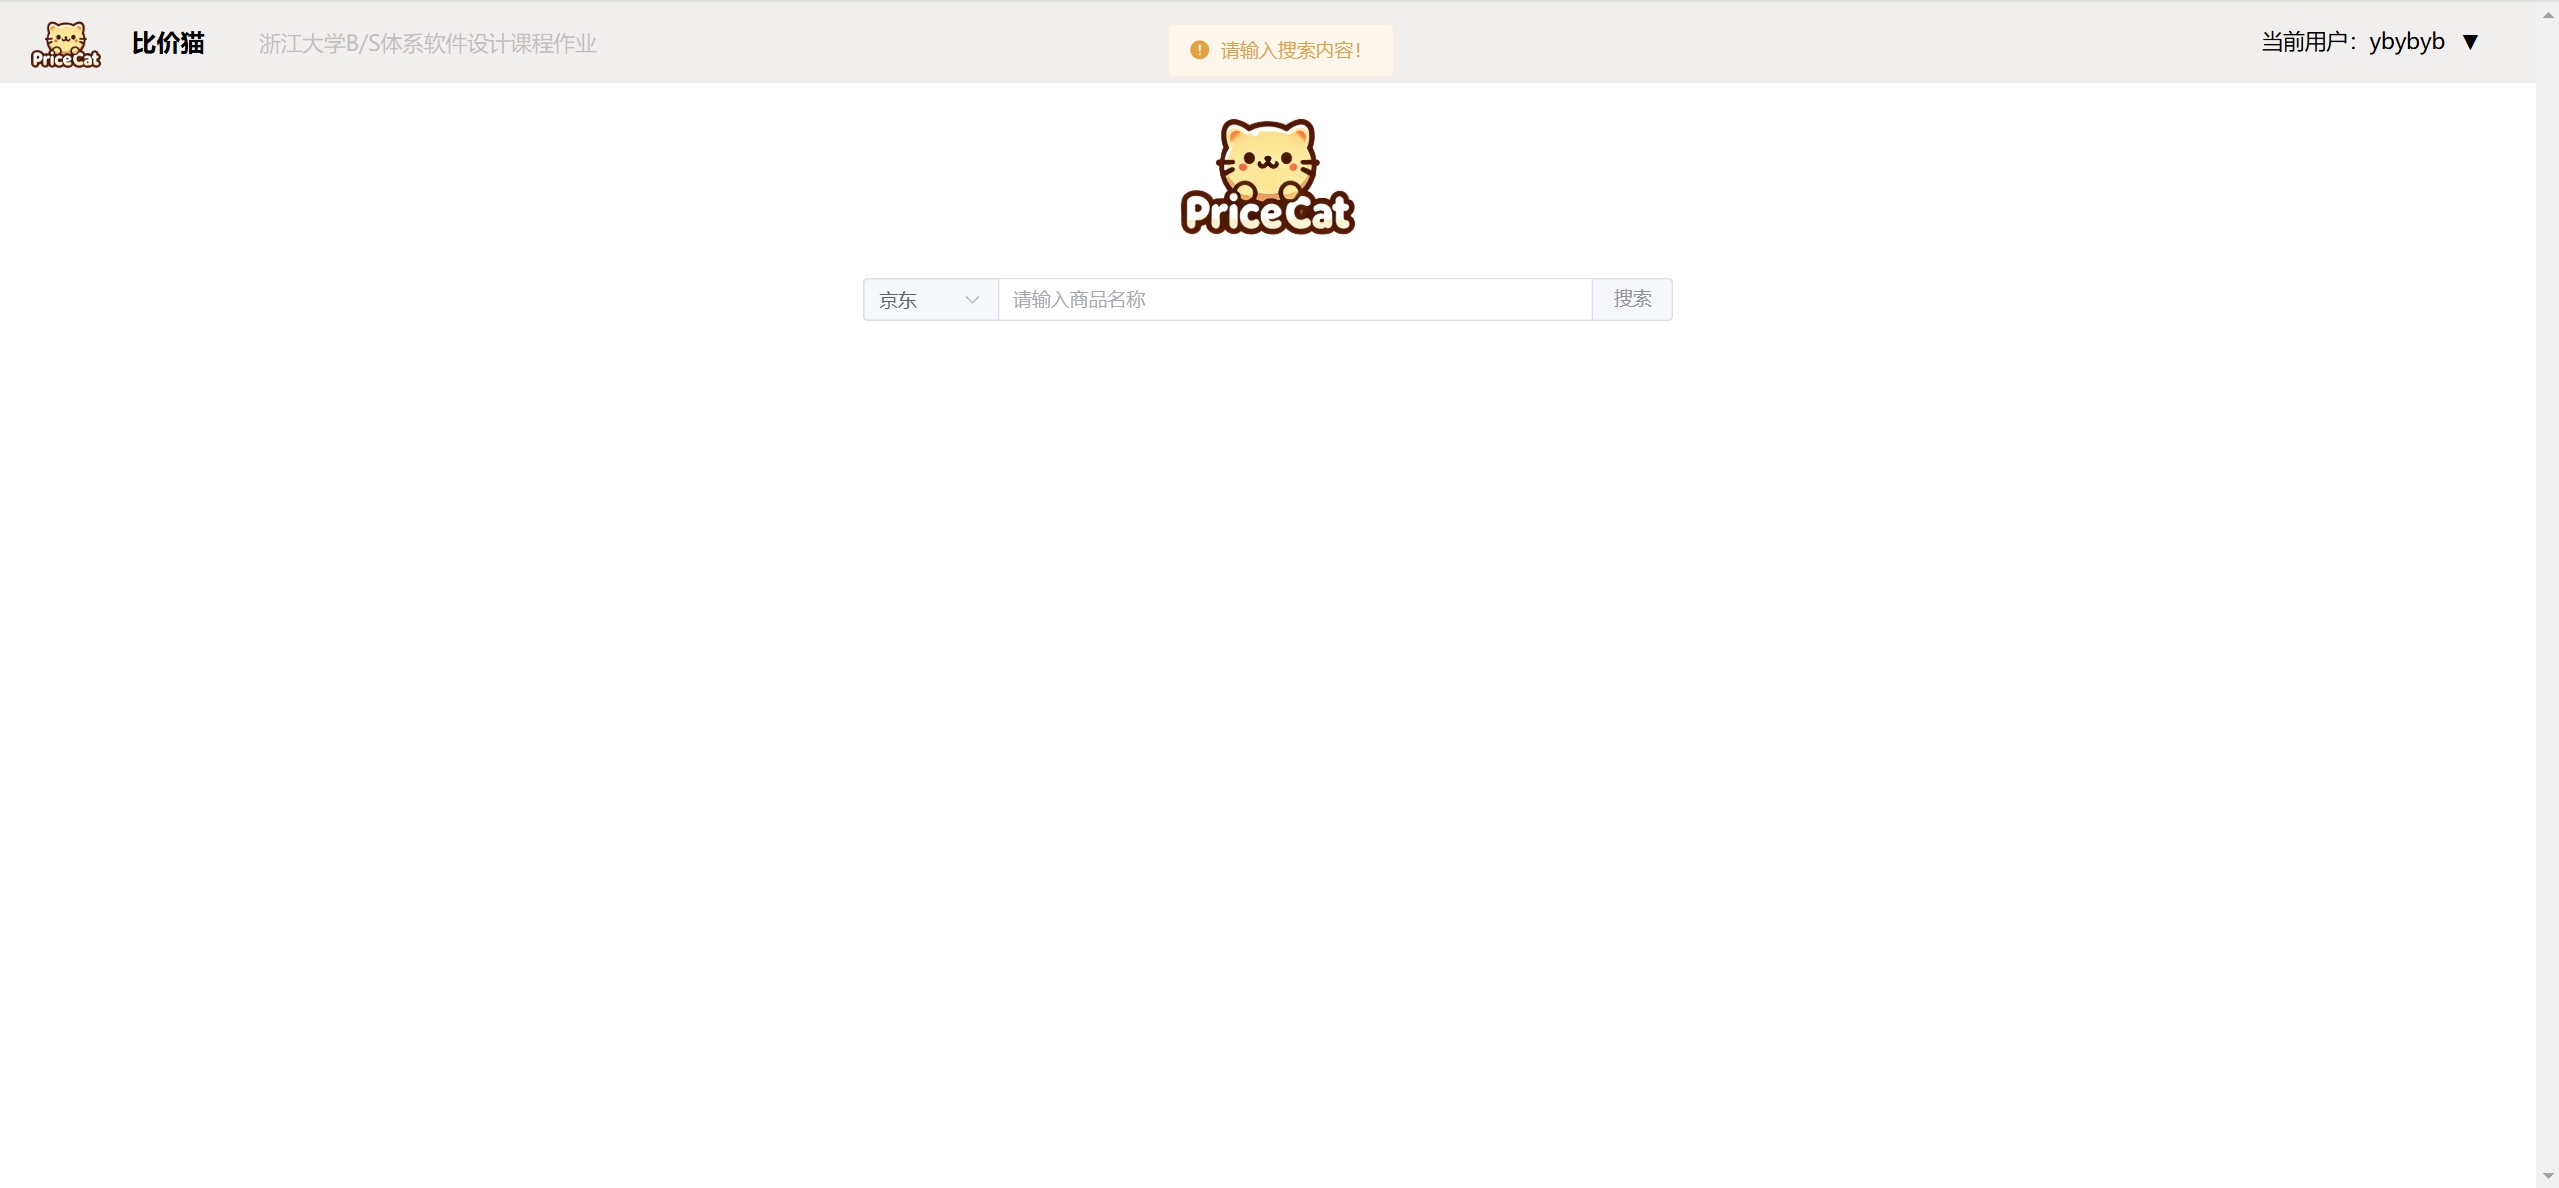
\includegraphics[width=1\textwidth]{./picture/商品查询边界值2.png}
\end{figure}

\section{安全性测试}

\subsection{SQL注入}
在登录页面输入SQL注入语句，不能成功登录。
\begin{figure}[H]
  \centering
  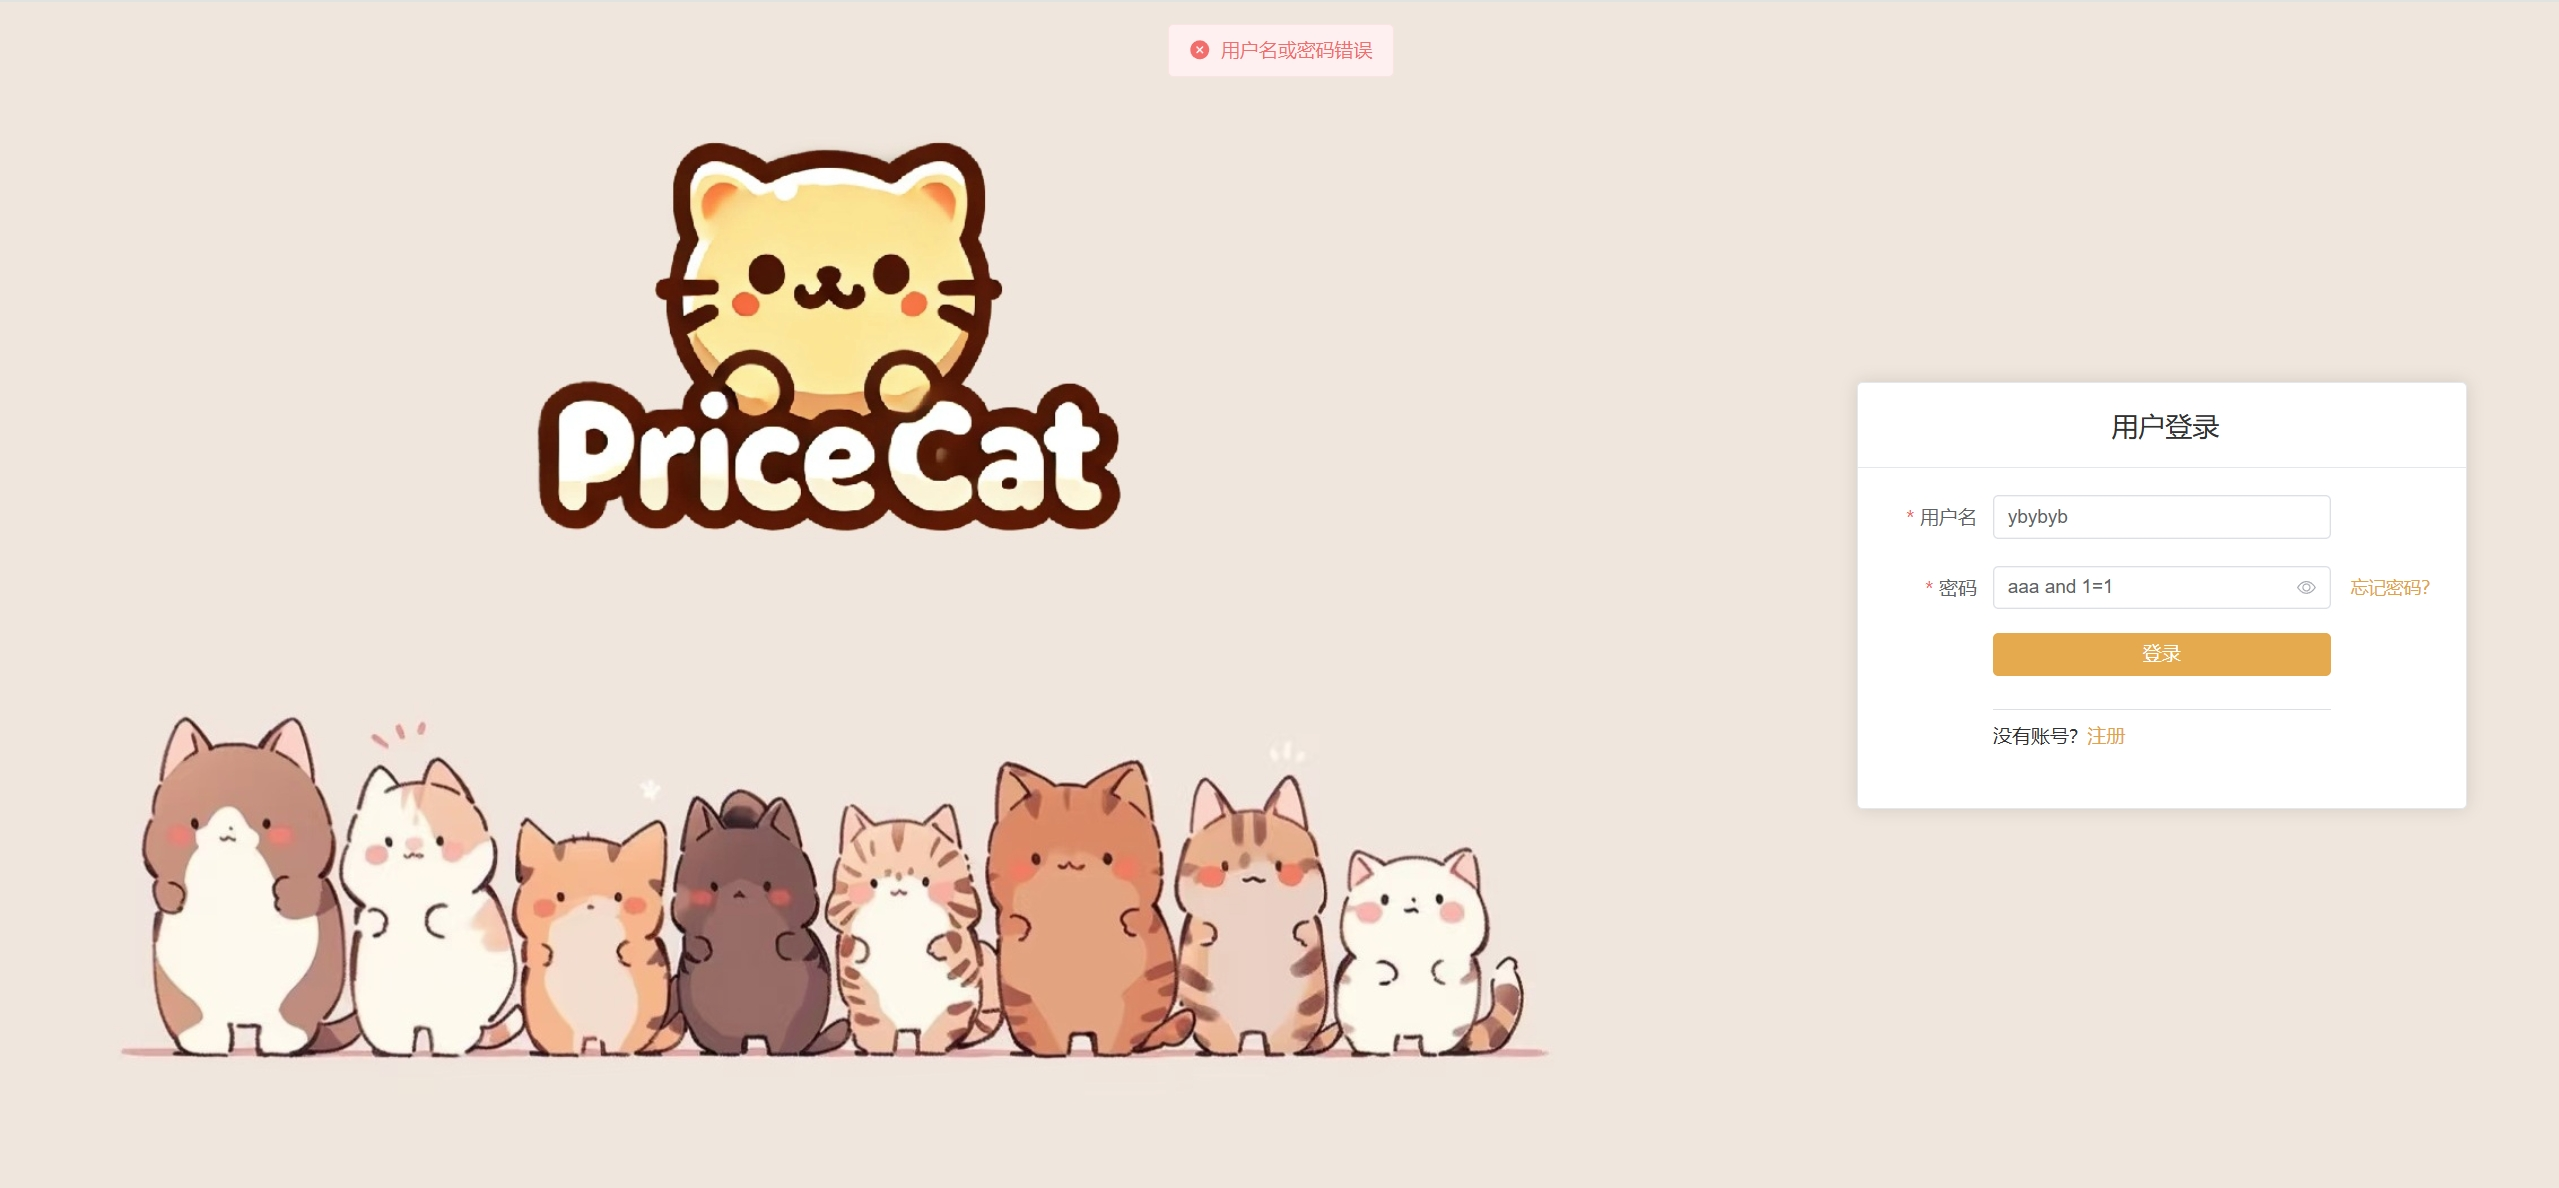
\includegraphics[width=1\textwidth]{./picture/SQL注入.png}
\end{figure}

\subsection{非法访问}
在未登录状态下使用URL直接使用搜索功能，不能查询到商品信息。
\begin{figure}[H]
  \centering
  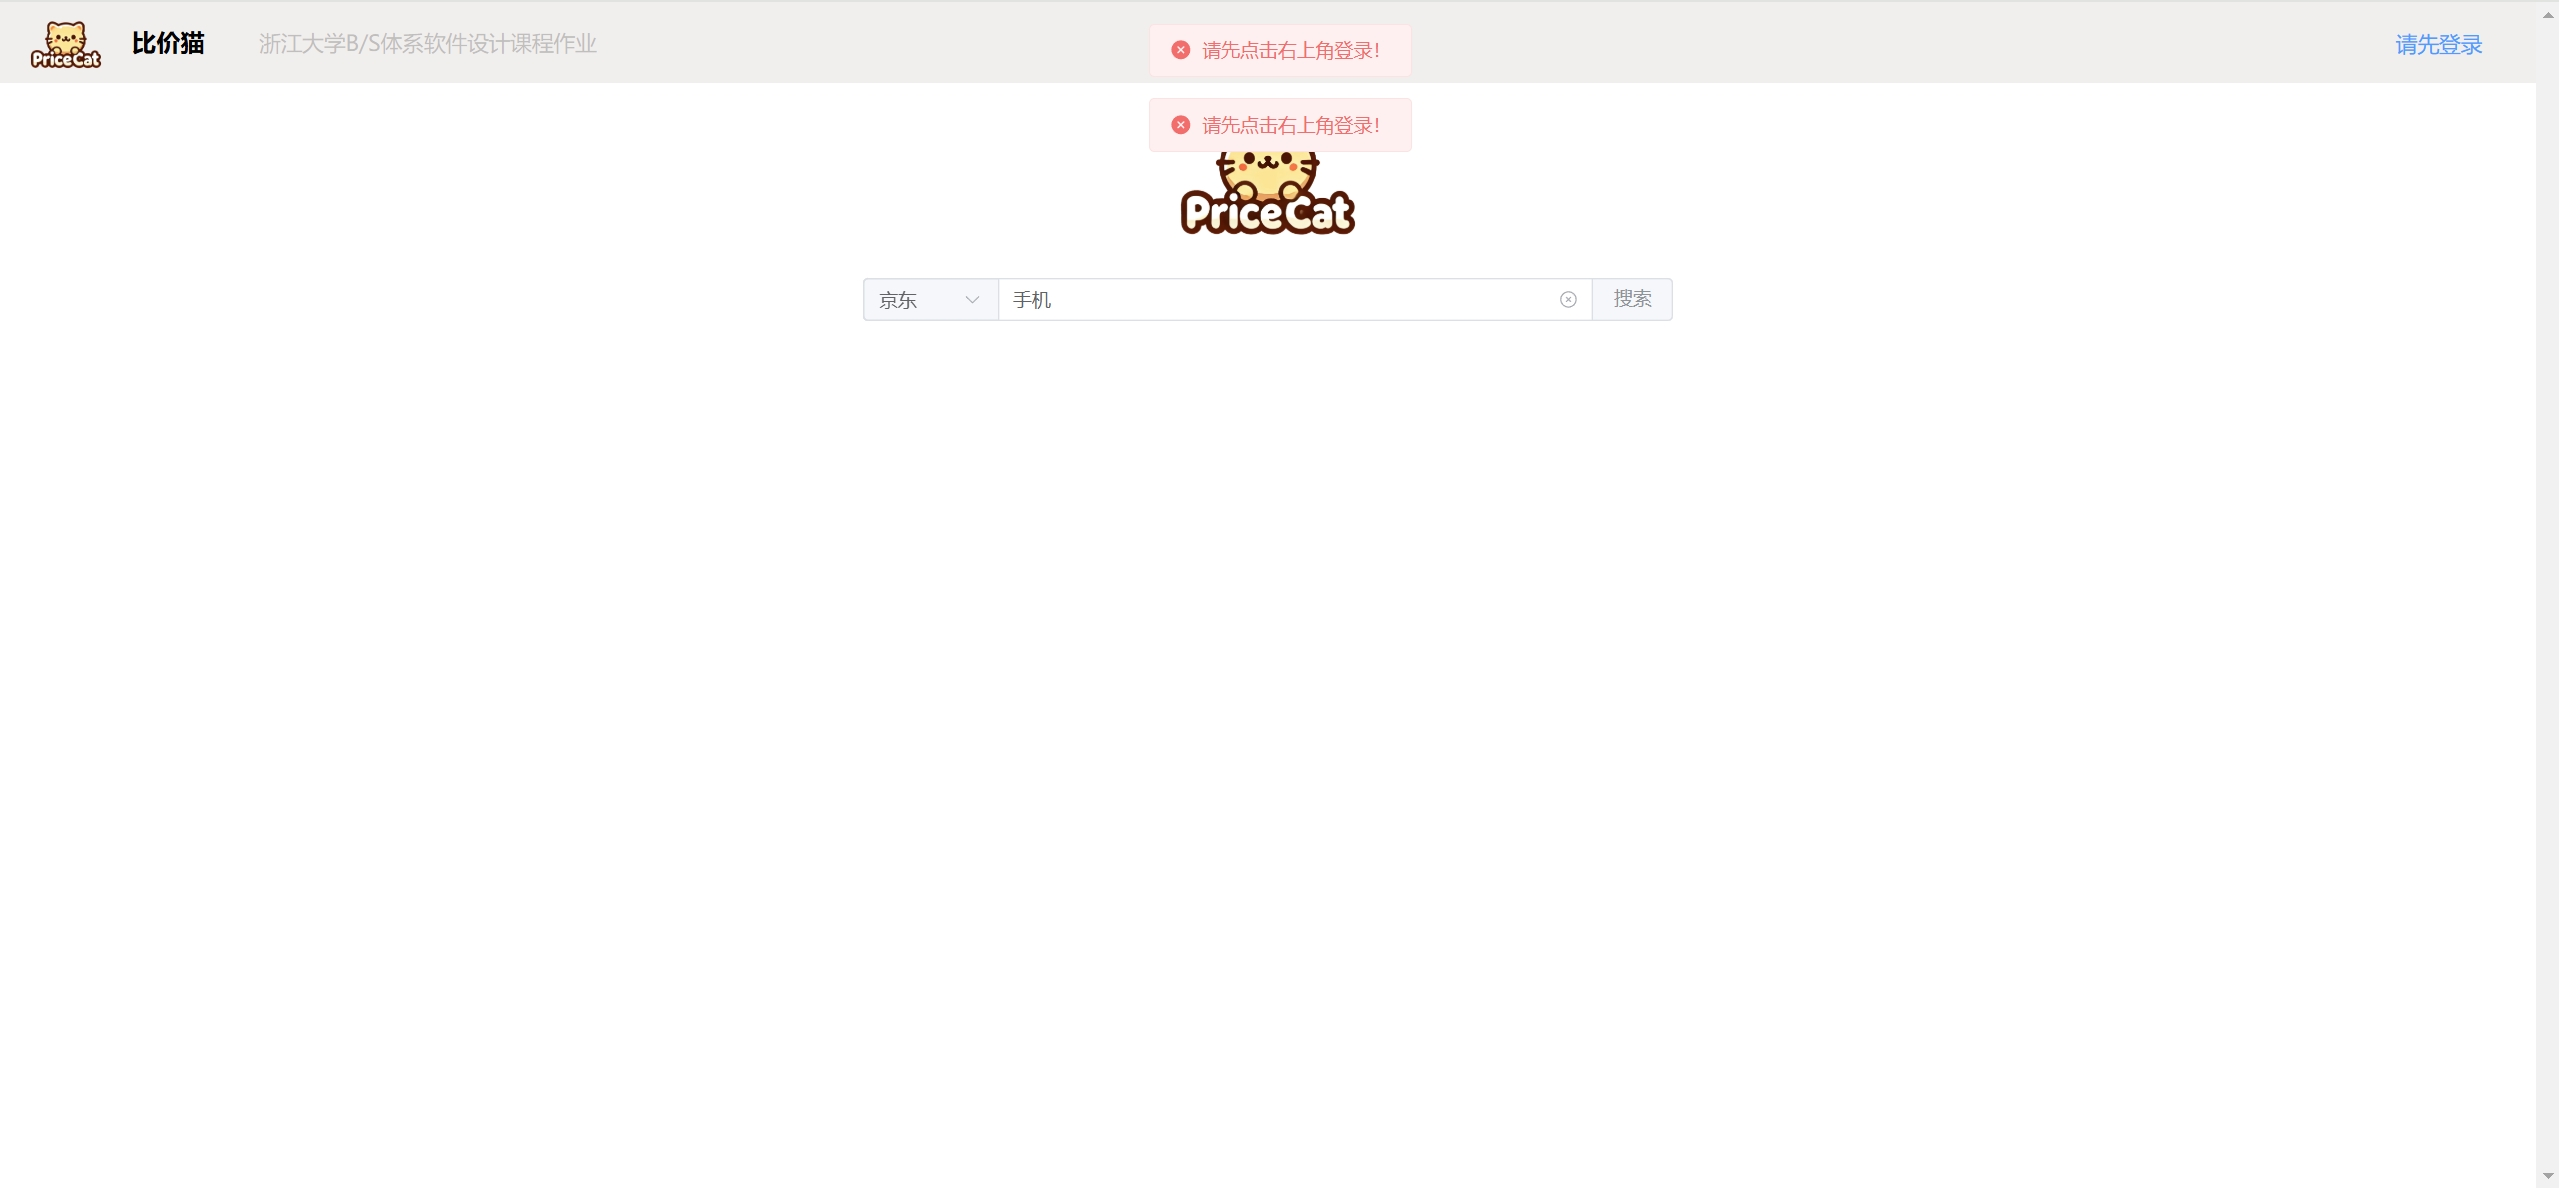
\includegraphics[width=1\textwidth]{./picture/非法访问1.png}
\end{figure}

在未登录状态下使用URL直接访问用户主页，不能查看和修改用户信息。
\begin{figure}[H]
  \centering
  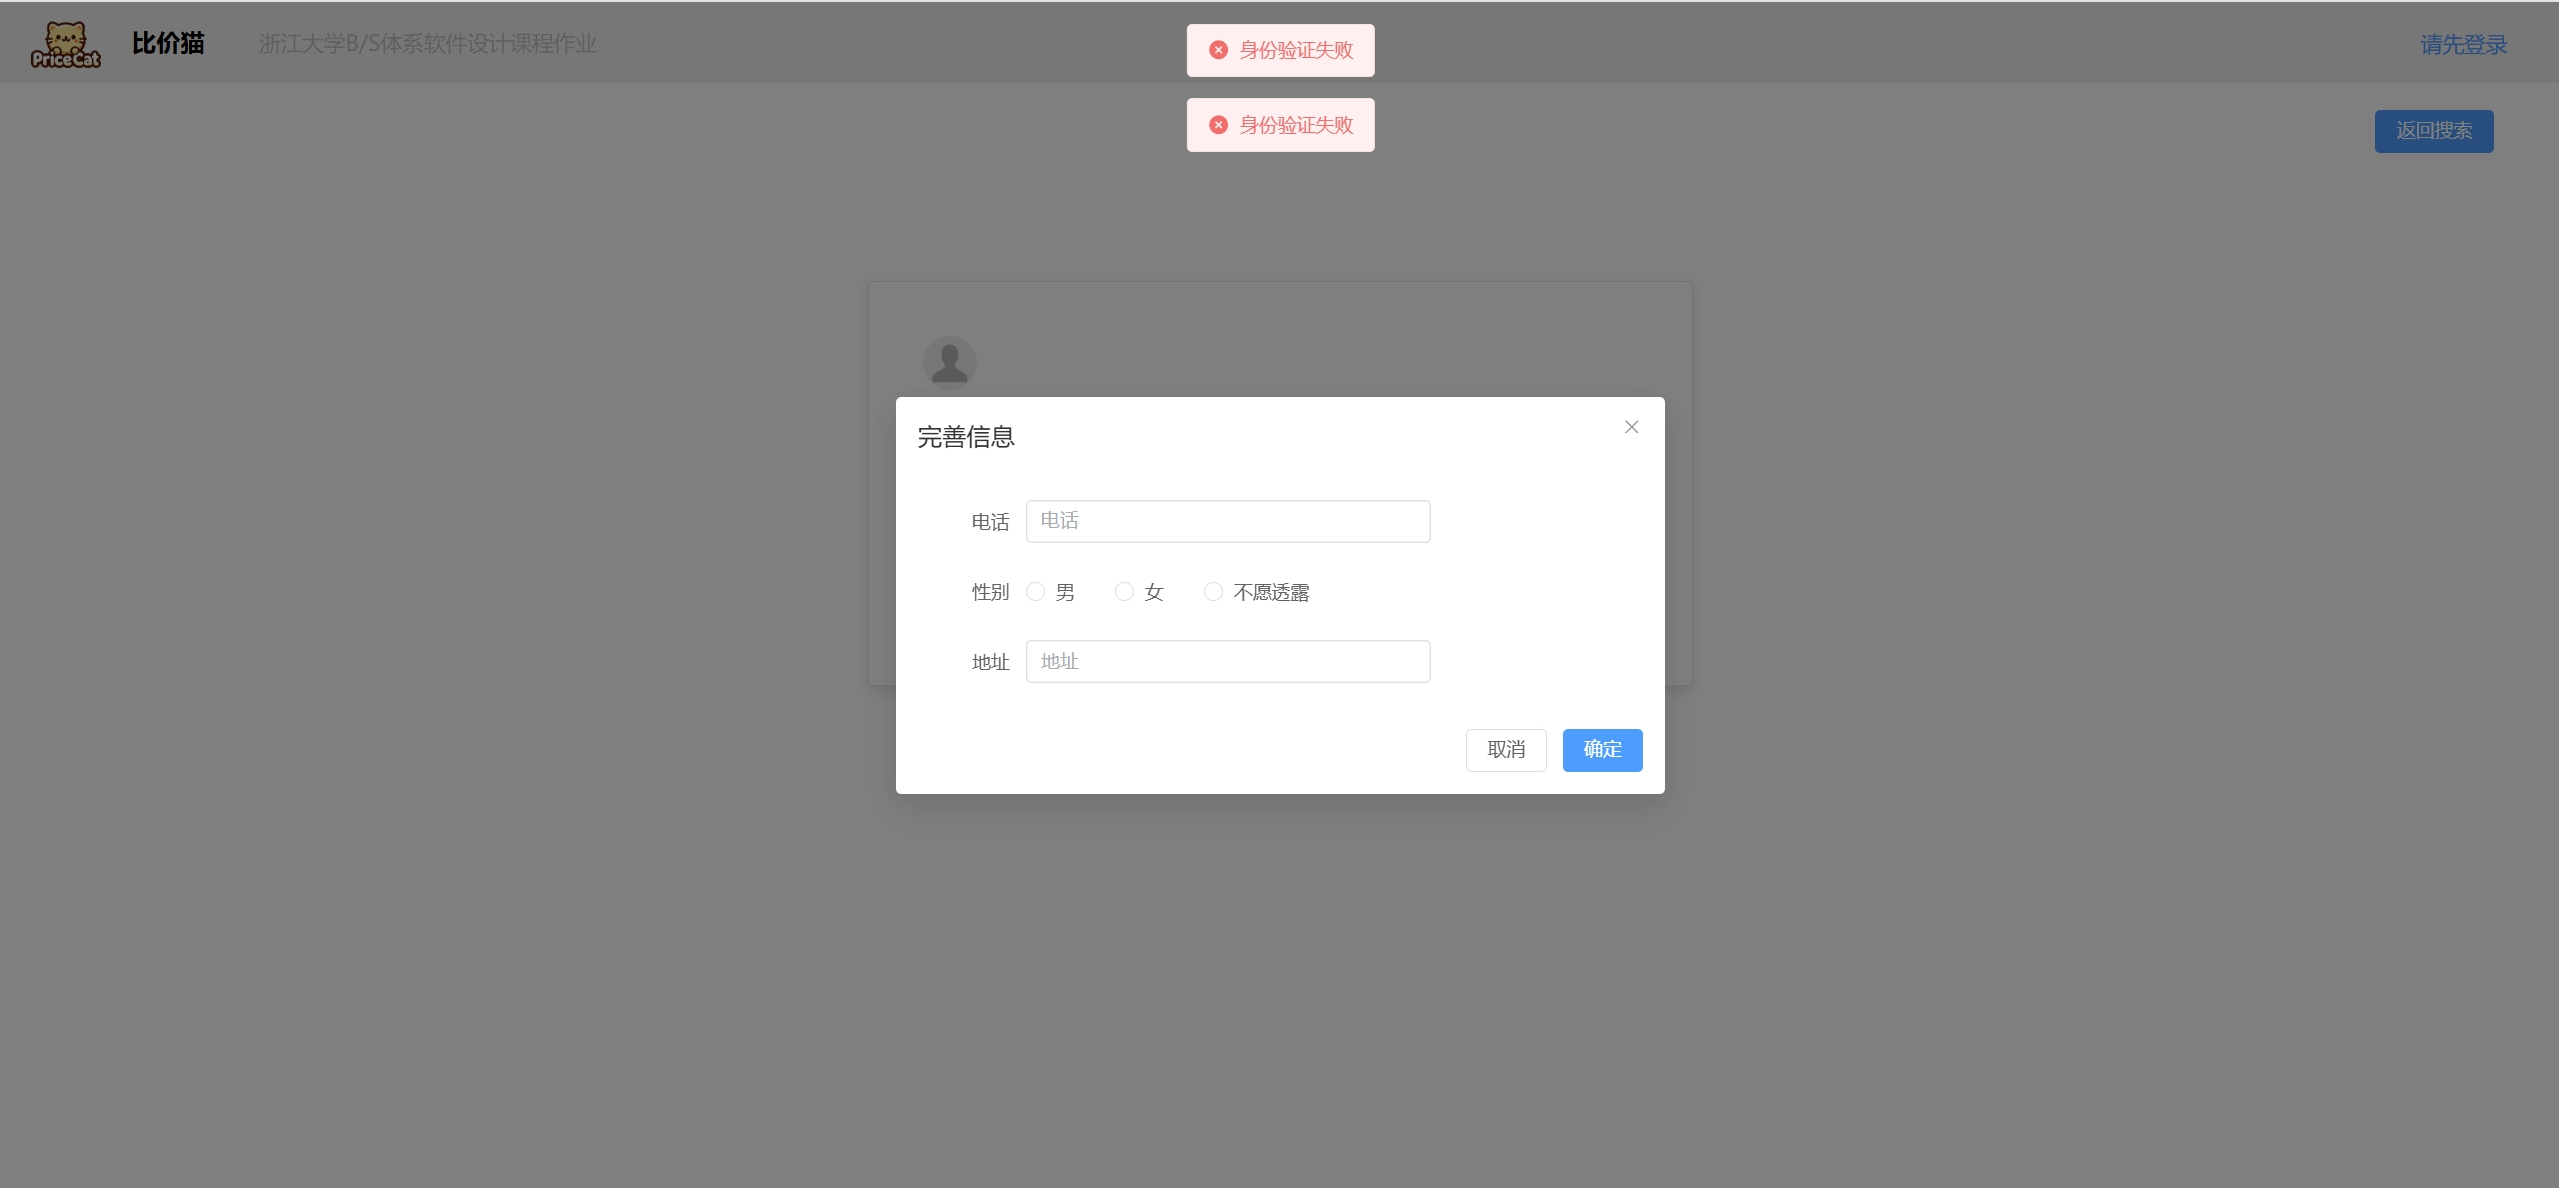
\includegraphics[width=1\textwidth]{./picture/非法访问2.png}
\end{figure}

\section{测试总结}

\subsection{优点}

经过基本的功能测试、边界值测试和安全性测试，系统的功能基本实现，能够正常使用用户注册登录、商品价格查询、商品详情与历史价格展示、降价提醒功能等功能。同时移动端的适配也较为友好，能够保证用户体验。同时，系统在安全性方面也有一定的保障，能够防止SQL注入和非法访问等安全问题。

\subsection{不足}

由于是单人完成的项目，测试的覆盖面较窄，可能存在一些未发现的问题。同时，由于工具使用的不熟练，项目没有做性能测试，可能存在性能问题。另外，由于时间有限，项目的功能也没有做太多的扩展，比如商品的筛选、排序等功能，还有待完善。

\end{document}